\documentclass[11pt]{article}
\usepackage{amsmath,amssymb,amsfonts,latexsym,graphicx,amsthm}
\usepackage{fullpage,color}
%\usepackage{text}
%\usepackage{algo}
\usepackage{setspace}
\usepackage{epstopdf}
\usepackage{url}
\usepackage{hyperref}
\usepackage{cleveref}
\usepackage{comment}
\usepackage[linesnumbered,boxed,ruled,vlined]{algorithm2e}
\usepackage{framed}
\usepackage[shortlabels]{enumitem}
\usepackage{tikz}
\usetikzlibrary{backgrounds}
\usetikzlibrary{decorations.pathreplacing,calligraphy}
\usetikzlibrary{decorations.pathmorphing}




%\pagestyle{empty}

\usepackage[margin=1in]{geometry}

\begin{comment}
\setlength{\oddsidemargin}{0in}
\setlength{\topmargin}{0in}
\setlength{\textwidth}{6.5in}
\setlength{\textheight}{8.5in}
\end{comment}

\newtheorem{fact}{Fact}
\newtheorem{theorem}{Theorem}[section]
\newtheorem{remark}[theorem]{Remark}
\newtheorem{lemma}[theorem]{Lemma}
\newtheorem{definition}{Definition}[section]
\newtheorem{corollary}[theorem]{Corollary}
\newtheorem{claim}[theorem]{Claim}
\newtheorem{observation}[theorem]{Observation}
\newtheorem{question}{Question}[section]
\newtheorem{invariant}{Invariant}[section]
\newtheorem{hypothesis}{Hypothesis}[section]

\newenvironment{note}[1]{\medskip\noindent \textbf{#1:}}%
        {\medskip}

\newcommand{\etal}{{\em et al.}\ }
\newcommand{\assign}{\leftarrow}
%\newcommand{\eps}{\epsilon}

%\newcommand{\opt}{\textrm{\sc OPT}}
\newcommand{\script}[1]{\mathcal{#1}}
%\newcommand{\ceil}[1]{\lceil #1 \rceil}
%\newcommand{\floor}[1]{\lfloor #1 \rfloor}

%\newcommand{\dist}{\mathbf{dist}}
\newcommand{\ball}{\mathsf{B}}
\newcommand{\balls}{\mathcal{B}}
\newcommand{\clusters}{\mathcal{B}}
%\newcommand{\vol}{\mathsf{vol}}
\newcommand{\tree}{\mathcal{T}}
\newcommand{\paths}{\Pi}
\newcommand{\err}{\mathsf{err}}
\newcommand{\val}{\mathsf{val}}
%\newcommand{\rk}{L}
\newcommand{\pathpart}{\textsf{PathPartition}\xspace}
\renewcommand{\epsilon}{\eps}
\newcommand{\brac}[1]{\left(#1\right)}

\newcommand{\tnote}[1]{\textcolor{orange}{{[Tianyi: #1]}}}


\begin{document}


\newcommand{\algline}{
	% \nointerlineskip \vspace{\baselineskip}%
	\rule{0.5\linewidth}{.1pt}\hspace{\fill}%
	\par\nointerlineskip \vspace{.1pt}
}
% Table: 
\newenvironment{tbox}{\begin{tcolorbox}[
		enlarge top by=5pt,
		enlarge bottom by=5pt,
		breakable,
		boxsep=0pt,
		left=4pt,
		right=4pt,
		top=10pt,
		boxrule=1pt,toprule=1pt,
		colback=white,
		arc=-1pt,
		%          drop shadow={black,opacity=1},
		% arc=0pt
		]%%
	}
	{\end{tcolorbox}}

%--------------------------------------------------------------
%--------------------------------------------------------------
%Comments
%--------------------------------------------------------------
%--------------------------------------------------------------


\newenvironment{proofof}[1]{\noindent{\bf Proof of #1.}}
{\hspace*{\fill}\stopproof}

\newenvironment{properties}[2][0]
{\renewcommand{\theenumi}{#2\arabic{enumi}}
	\begin{enumerate} \setcounter{enumi}{#1}}{\end{enumerate}\renewcommand{\theenumi}{\arabic{enumi}}}

\newif\ifnocomments
%\nocommentstrue

% \nocommentsfalse %Uncommenting this  gives the comments version
%%%

\ifnocomments

\newcommand{\znote}[1]{}


\else
\newcommand{\znote}[1]{\textcolor{red}{\sc{[ZT: #1]}}}

\fi



%--------------------------------------------------------------
%--------------------------------------------------------------
%Special Notations
%--------------------------------------------------------------
%--------------------------------------------------------------

\newcommand{\tG}{\textbf{G}}
\newcommand{\tH}{\textbf{H}}
\newcommand{\tE}{\textbf{E}'}
\newcommand{\tC}{\textbf{C}}
\newcommand{\tphi}{\bm{\phi}}
\newcommand{\tpsi}{\bm{\psi}}
\newcommand{\tSigma}{\bm{\Sigma}}
\newcommand{\tB}{\tilde B}
\newcommand{\dout}{D_{\mbox{\tiny{out}}}}
\newcommand{\notF}{\overline{F}}


%--------------------------------------------------------------
%--------------------------------------------------------------
%Complexity Classes
%--------------------------------------------------------------
%--------------------------------------------------------------
\renewcommand{\P}{\mbox{\sf P}}
\newcommand{\NP}{\mbox{\sf NP}}
\newcommand{\PCP}{\mbox{\sf PCP}}
\newcommand{\ZPP}{\mbox{\sf ZPP}}
%\newcommand{\polylog}[1]{\mathrm{polylog(#1)}}
\newcommand{\DTIME}{\mbox{\sf DTIME}}
\newcommand{\opt}{\mathsf{OPT}}
\newcommand{\optcro}{\mathsf{OPT}_{\mathsf{cr}}}
\newcommand{\optcrors}{\mathsf{OPT}_{\mathsf{cnwrs}}}
%--------------------------------------------------------------
%--------------------------------------------------------------
%Sets
%--------------------------------------------------------------
%--------------------------------------------------------------
\newcommand{\set}[1]{\left\{ #1 \right\}}
\newcommand{\sse}{\subseteq}
\newcommand{\B}{{\mathcal{B}}}
\newcommand{\tset}{{\mathcal T}}
\newcommand{\vset}{{\mathcal V}}
\newcommand{\uset}{{\mathcal U}}
\newcommand{\iset}{{\mathcal{I}}}
\newcommand{\pset}{{\mathcal{P}}}
\newcommand{\nset}{{\mathcal{N}}}
\newcommand{\dset}{{\mathcal{D}}}
\newcommand{\tpset}{\tilde{\mathcal{P}}}
\newcommand{\qset}{{\mathcal{Q}}}
\newcommand{\tqset}{\tilde{\mathcal{Q}}}
\newcommand{\lset}{{\mathcal{L}}}
\newcommand{\bset}{{\mathcal{B}}}
\newcommand{\tbset}{\tilde{\mathcal{B}}}
\newcommand{\aset}{{\mathcal{A}}}
\newcommand{\cset}{{\mathcal{C}}}
\newcommand{\fset}{{\mathcal{F}}}
\newcommand{\mset}{{\mathcal M}}
\newcommand{\jset}{{\mathcal{J}}}
\newcommand{\xset}{{\mathcal{X}}}
\newcommand{\wset}{{\mathcal{W}}}
\newcommand{\gset}{{\mathcal{G}}}
\newcommand{\oset}{{\mathcal{O}}}
\newcommand{\yset}{{\mathcal{Y}}}
\newcommand{\rset}{{\mathcal{R}}}
\newcommand{\I}{{\mathcal I}}
\newcommand{\hset}{{\mathcal{H}}}
\newcommand{\sset}{{\mathcal{S}}}
\newcommand{\zset}{{\mathcal{Z}}}
\newcommand{\notu}{\overline U}
\newcommand{\vol}{\operatorname{vol}}
\newcommand{\nots}{\overline S}
\newcommand{\eint}{E^{\tiny\mbox{int}}}
\newcommand{\event}{{\cal{E}}}
\newcommand{\floor}[1]{\ensuremath{\left\lfloor#1\right\rfloor}}
\newcommand{\ceil}[1]{\ensuremath{\left\lceil#1\right\rceil}}
%--------------------------------------------------------------
%--------------------------------------------------------------

\newcommand{\marcon}{{\mathsf{MC}}}
\newcommand{\cov}{{\mathsf{cov}}}
\newcommand{\mst}{{\mathsf{MST}}}
\newcommand{\card}[1]{|#1|}
\newcommand{\coi}{{\mathsf{COI}}}

\newcommand{\med}{\mathcal{C}}
\newcommand{\avg}{\overline{\lambda}}



%--------------------------------------------------------------
%--------------------------------------------------------------
%For Metric TSP
%--------------------------------------------------------------
%--------------------------------------------------------------
\newcommand{\cover}{\textsf{cover}}
\newcommand{\eps}{\varepsilon}
\newcommand{\bfs}{\textnormal{\textsf{BFS}}}
\newcommand{\pbfs}{\textnormal{\textsf{BFS}}}
\newcommand{\lv}{\textsf{lv}}
\newcommand{\tsp}{\mathsf{TSP}}
\newcommand{\gtsp}{\textsf{GTSP}}
\newcommand{\ebt}{\tset}
\newcommand{\eb}{\textsf{EB}}
\newcommand{\optmst}{\textsf{MST}}
\newcommand{\defi}{\textsf{def}}
\newcommand{\ord}{\textsf{ord}}
\newcommand{\rc}{\textnormal{\textsf{rc}}}
\newcommand{\dist}{\textnormal{\textsf{dist}}}
\newcommand{\cost}{\textnormal{\textsf{cost}}}
\newcommand{\bw}{\textsf{bw}}
\newcommand{\local}{\textsf{Local}}
\newcommand{\pseudo}{\textsf{Pseudo-IP}}
\newcommand{\vin}{v^{\textnormal{\textsf{in}}}}
\newcommand{\vout}{v^{\textnormal{\textsf{out}}}}
\newcommand{\diam}{\textsf{diam}}
\newcommand{\expect}{\mathbb{E}}
\newcommand{\proover}{\pi_{\textsf{Overwrite}}}
\newcommand{\promst}{\pi_{\textsf{MST}}}
\newcommand{\protsp}{\pi_{\textsf{TSP}}}
\newcommand{\mstest}{\textsf{MST}_{\textsf{apx}}}
\newcommand{\tspest}{\textsf{TSP}_{\textsf{apx}}}
\newcommand{\proind}{\pi_{\textsf{Index}}}
\newcommand{\ind}{\textsf{Index}}
\newcommand{\distIND}{\mathcal{D}_{\textsf{Index}}}
\newcommand{\distMST}{\mathcal{D}_{\textsf{MST}}}
\newcommand{\ic}{\textnormal{\textsf{IC}}}
\newcommand{\cc}{\textnormal{\textsf{CC}}}
\newcommand{\tvd}[2]{\ensuremath{\Delta_{\textnormal{\texttt{TV}}}(#1,#2)}}
\newcommand{\dkl}[2]{\ensuremath{D_{\textnormal{\textsf{KL}}}(#1 \| #2)}}

\newcommand{\hel}{h}
\newcommand{\II}{I}
\newcommand{\HH}{H}

\newcommand{\RV}[1]{\mathbf{#1}}
\newcommand{\prot}{\ensuremath{\Pi}}
\newcommand{\Prot}{\ensuremath{\Pi}}
\newcommand{\findmiss}{\sf{FindBit}}
\newcommand{\overwrite}{\sf{Overwrite}}
\newcommand{\distfind}{\mathcal{D}_{\textsf{FindBit}}}
\newcommand{\distover}{\mathcal{D}_{\textsf{Overwrite}}}
\newcommand{\temp}{\textsf{temp}}
\newcommand{\IA}{\textsf{IA}}
\newcommand{\IB}{\textsf{IB}}


\newcommand{\row}{\textsf{Row}}
\newcommand{\col}{\textsf{Col}}
\newcommand{\alg}{\ensuremath{\mathsf{Alg}}\xspace}
\newcommand{\algrc}{\ensuremath{\mathsf{AlgURC}}\xspace}
\newcommand{\minkcut}{minimum weight $k$-cut\xspace}
\newcommand{\wts}{\omega}
\newcommand{\Eout}{E^{\textnormal{out}}}

\newcommand{\sunf}{\mathsf{sf}}



\begin{titlepage}
	
\title{Almost-Optimal Sublinear Additive Spanners\footnote{Extended abstract appeared in STOC 2023.}}
\author{Zihan Tan \thanks{DIMACS, Rutgers University, \href{}{zihantan1993@gmail.com. This author is supported by a grant to DIMACS from the Simons Foundation (820931).}} \and Tianyi Zhang \thanks{Tel Aviv University, \href{}{tianyiz21@tauex.tau.ac.il. This author is supported by the European Research Council (ERC) under the European Union’s Horizon 2020 research and innovation programme (grant agreement No 803118 UncertainENV).}}}
	\date{}
	\maketitle
	
	\thispagestyle{empty}
	
\begin{abstract}
Given an undirected unweighted graph $G = (V, E)$ on $n$ vertices and $m$ edges, a subgraph $H\subseteq G$ is a \emph{spanner} of $G$ with stretch function $f: \mathbb{R}_+ \rightarrow \mathbb{R}_+$, if for every pair $s, t$ of vertices in $V$,  $\dist_{H}(s, t)\le f(\dist_{G}(s, t))$. When $f(d) = d + o(d)$, $H$ is called a \emph{sublinear additive spanner}; when $f(d) = d + o(n)$, $H$ is called an \emph{additive spanner}, and $f(d) - d$ is usually called the \emph{additive stretch} of $H$.

As our primary result, we show that for any constant $\delta>0$ and constant integer $k\geq 2$, every graph on $n$ vertices has a sublinear additive spanner with stretch function $f(d)=d+O(d^{1-1/k})$ and $O\big(n^{1+\frac{1+\delta}{2^{k+1}-1}}\big)$ edges. When $k = 2$, this improves upon the previous spanner construction with stretch function $f(d) = d + O(d^{1/2})$ and $\tilde{O}(n^{1+3/17})$ edges [Chechik, 2013]; for any constant integer $k\geq 3$, this improves upon the previous spanner construction with stretch function $f(d) = d + O(d^{1-1/k})$ and $O\bigg(n^{1+\frac{(3/4)^{k-2}}{7 - 2\cdot (3/4)^{k-2}}}\bigg)$ edges [Pettie, 2009]. Most importantly, the size of our spanners almost matches the %unconditional
lower bound of $\Omega\big(n^{1+\frac{1}{2^{k+1}-1}}\big)$ [Abboud, Bodwin, Pettie, 2017], which holds for all compression schemes achieving the same stretch function.

As our second result, we show a new construction of additive spanners with stretch $O(n^{0.403})$ and $\tilde{O}(n)$ edges, which slightly improves upon the previous stretch bound of $O(n^{3/7+\eps})$ achieved by linear-size spanners [Bodwin and Vassilevska Williams, 2016]. An additional advantage of our spanner is that it admits a subquadratic construction runtime of $\tilde{O}(m + n^{13/7})$, while the previous construction in [Bodwin and Vassilevska Williams, 2016] requires all-pairs shortest paths computation which takes $O(\min\{mn, n^{2.373}\})$ time.
	
	% Our approach is a strengthening of the old clustering + path buying method, that discovered and exploited the connection between additive spanners and subset/pairwise additive spanners.
\end{abstract}

\end{titlepage}

\begin{spacing}{1.3}
\tableofcontents
\end{spacing}

\thispagestyle{empty}
\clearpage
\setcounter{page}{1}

\newpage

\section{Introduction}

The increasing complexity of source code poses a key challenge to the reliability of large-scale software systems. Software bugs in these systems can lead to safety issues~\cite{bug_safety} for users around the world as well as cause non-negligible financial losses~\cite{bug_loss}. As such, developers have to spend a large amount of time and effort on bug fixing. Consequently, \aprfull (\apr), designed to automatically generate patches to fix software bugs, has attracted wide attention from both academia and industry~\cite{long2016prophet, legoues2012genprog, long2015spr, lou2020can, tufano2018empstudy}. 


To achieve \apr, one popular approach is known as Generate-and-Validate (G\&V)~\cite{qi2015gv, ghanbari2019prapr, lou2020can, le2016hdrepair, legoues2012genprog, wen2018capgen, hua2018sketchfix, martinez2016astor, koyuncu2020fixminder, liu2019tbar, liu2019avatar}, which is typically based on the following pipeline: First, fault localization techniques~\cite{wong2016fl, abreu2007ochiai, zhang2013injecting, papadakis2015metallaxis, li2019deepfl, li2017transforming} are applied to determine the suspicious locations in programs where bugs are likely to exist. Then, the buggy locations are used by the \apr tools to generate a list of patches that replace buggy lines with correct lines. Afterward, each patch is validated against the original test suite to identify any \emph{plausible patches} (i.e., passing all tests in the test suite). Finally, to determine the \emph{correct patches}, developers examine the list of plausible patches to see if any of them can correctly fix the bug. 

Traditional \apr tools can mainly be categorized into heuristic-based~\cite{legoues2012genprog, le2016hdrepair, wen2018capgen}, constraint-based~\cite{mechtaev2016angelix, le2017s3, demacro2014nopol, long2015spr} and \template~\cite{ghanbari2019prapr, hua2018sketchfix, martinez2016astor, liu2019tbar, liu2019avatar}. Among these traditional tools, \template \apr tools~\cite{ghanbari2019prapr, liu2019tbar, benton2020effectiveness} have been able to achieve state-of-the-art results. \Template \apr tools typically leverage pre-defined templates (e.g., adding a nullness check) for bug fixing. However, since these fix templates are typically handcrafted, the number and types of bugs they are able to fix can be limited. 



To address the limitations of traditional \apr, researchers have proposed various \learning \apr tools~\cite{li2020dlfix, chen2018sequencer, jiang2021cure, lutellier2020coconut, zhu2021recoder, ye2022rewardrepair} based on the \nmtfull (\nmt) architecture~\cite{sutskever2014mt} where the input is the buggy code snippets and the goal is to translate the buggy code snippets into a fixed version. To accomplish this, \learning \apr tools require supervised training datasets with pairs of both buggy and fixed code snippets in order to learn how to perform this translation step. These training data are usually obtained by mining historical bug fixes using heuristics/keywords~\cite{dallmeier2007benchmark}, which can be imprecise for identifying bug-fixing commits; even the actual bug-fixing commits can include irrelevant code changes, leading to further pollution in the dataset~\cite{xia2022alpharepair}.
% 
Moreover, it can be hard for such \apr tools to generalize and fix bug types unseen during training. 



To better leverage recent advances in \plmfull{s} (\plm{s}), researchers~\cite{xia2022alpharepair, xia2023repairstudy, kolak2022patch, prenner2021codexws} have directly applied \plm{s} to generate patches without bug-fixing datasets. These \llm-based \apr tools work by either directly generating a complete code function~\cite{prenner2021codexws, xia2023repairstudy} or predict/infill the correct code snippet given its surrounding context~\cite{xia2022alpharepair, xia2023repairstudy}. By directly using \llm{s} that are pre-trained on billions of open-source code snippets, \llm-based \apr tools can achieve state-of-the-art performance on many repair datasets~\cite{xia2022alpharepair}. 


% 
%
%

Traditional \apr tools have long used the insight of the \emph{plastic surgery hypothesis}~\cite{barr2014plastic} where it states that the code ingredients to fix a bug already exist within the same project. Traditional \apr tools have manually designed pattern-~\cite{ghanbari2019prapr, saha2017elixir} or heuristic-based~\cite{jiang2018simfix, legoues2012genprog} approaches to finding and using such relevant code ingredients to generate fixes for bugs. However, the plastic surgery hypothesis has been largely ignored in \llm-based \apr. In fact, \llm provides a unique opportunity to fully automate the plastic surgery hypothesis idea via fine-tuning (learning project-specific information via model updates from the buggy project) and prompting (directly providing relevant code ingredients to the model), and make it directly applicable to different languages (since the \llm{s} are typically multi-lingual).%
Moreover, despite the intensive manual efforts involved, traditional \apr tools still cannot fully leverage project-specific information due to large search space for leveraging/composing existing code ingredients. In contrast, the project-specific information can effectively leveraged by \llm{s} due to their power in code understanding/vectorization, e.g., even partial/imprecise information may still guide \llm{s} in correct patch generation!
 To this end, we ask the question: \emph{How useful is the plastic surgery hypothesis in the era of \plm{s}}?








\mypara{Our Work.} To answer the question, we present \ourtech{\xspace} -- a \llm-based approach that automatically utilizes the plastic surgery hypothesis by systematically combining multiple fine-tuning and prompting strategies for \apr. \ourtech fine-tunes \plm{s} using two novel domain-specific training strategies: \textbf{\epfinetune} -- we fine-tune using the original buggy project by aggressively masking out a high percentage of tokens, which allows \plm to learn project-specific code tokens and programming styles; and \textbf{\rofinetune} -- which only masks out a single continuous code sequence per training sample, allowing the model to get used to the final \csapr task of predicting a single continuous code sequence. Furthermore, we directly leverage the ability for \plm{s} to understand natural language instructions and introduce a novel prompting strategy, \textbf{\idprompting}, which uses information retrieval and static analysis to obtain a list of relevant identifiers for the buggy lines. While such relevant identifiers are critical for fixing some difficult bugs, they may not be seen by the \llm during inference due to limited context window size. Through the use of prompting, we directly tell the model to use these extracted identifiers (relevant code ingredients) to generate the correct code. Finally, to perform repair, we combine all four model variants (including the base model, both fine-tuned models and the base model with prompting) for the final repair.





While our insight of leveraging the plastic surgery hypothesis for \llm-based \apr is generalizable across different types of \plm{s}, to implement \ourtech, we choose a recent \plm{\xspace}, \ctfive~\cite{wang2021codet5}, which is pre-trained on millions of open-source code snippets. \ctfive is an encoder-decoder model trained using \mspfull (\msp) objective where a percentage of tokens are masked out and each continuous masked token sequence is referred to as a masked span. Also, although we only extract relevant identifiers from the current buggy project (since this paper focuses on the plastic surgery hypothesis), our work can be easily extended to obtain other code information (such as relevant statements or functions) from other sources, such as  the massive pre-training corpora~\cite{husain2020codesearchnet} or historical bug-fixing datasets~\cite{jiang2019infer}, which can provide more coding knowledge for \llm{s}. Besides, although we mainly focus on using traditional string comparison algorithms for information retrieval in this paper, these techniques can be easily replaced by other frequency-based retrieval~\cite{robertson2009probabilistic} and neural search (or embedding-based search)~\cite{reimers2019sentence}.
  In summary, this paper makes the following contributions:


%


\begin{itemize}[noitemsep, leftmargin=*, topsep=0pt]
    \item \textbf{Dimension.} This paper is the first to revisit the important plastic surgery hypothesis in the era of \llm{s}. It opens up a new dimension for \llm-based \apr to incorporate previously neglected information from the buggy project itself to boost \apr performance. Furthermore, it demonstrates the promising future of retrieval-based prompting for modern \llm-based \apr.
    \item \textbf{Implementation.} We implement \ourtech based on the recent \ctfive model. We augment the model using two novel fine-tuning strategies: \epfinetune and \rofinetune, along with a novel prompting strategy based on information retrieval and static analysis: \idprompting. We combine the patches generated by all four models together and perform patch ranking to speed up \apr.% 
    \item \textbf{Evaluation Study.} We conduct an extensive evaluation against state-of-the-art \apr tools. On the widely studied \dfj 1.2 and 2.0 datasets~\cite{just2014dfj}, \ourtech is able to achieve the new state-of-the-art results of 89 and 44 correct bug fixes (15 and 8 more than best baseline) respectively.  Furthermore, we perform a broad ablation study to justify our design. \ourtech demonstrates for the first time that the plastic surgery hypothesis can substantially boost \llm-based \apr and advance state-of-the-art \apr, while being fully automated and general. Moreover, even partial/imprecise code ingredients may still effectively guide \llm{s} for \apr!
\end{itemize}


\section{Preliminaries}

\subsection{Lithography Simulation Model} \label{litho_model}
During the lithography process, an input mask $\mathbf{M}$ is projected through layers of optical lens onto a wafer plane. The intensity after optical system $\mathbf{I}$, namely the aerial image, leaves a coating on the wafer with photoresist to form the resulting pattern $\mathbf{Z}$. The conventional simulation of the lithography process is composed of 2 consecutive components: optical projection model and photoresist model. 

For the projection process, Hopkins diffraction model \cite{hopkins1951concept} has been widely used to analyze coherent imaging system mathematically. To avoid the computation complexity of the Hopkins model, a singular value decomposition model (SVD)-based approximation has been proposed by \cite{cobb1998fast} and became the mainstream fashion. In the SVD model, the Hopkins diffraction model can be decomposed into a sum of coherent systems based on eigenvalue decomposition:
\begin{equation}
    \mathbf{I}(x,y) = \sum_{k = 1}^{ N^{2}} w_{k} | \mathbf{M}(x,y) \otimes h_{k}(x,y) |^{2}, \quad x,y = 1,2,...N
\end{equation}
where $h_{k}$ is the $k$-th kernel and $w_{k}$ is the corresponding weight of the coherent system. "$\otimes$" denotes the convolution operator. \cite{gao2014mosaic} indicates the $K$-th order approximation:
\begin{equation}
    \mathbf{I}(x,y) \approx \sum_{k = 1}^{K} w_{k} | \mathbf{M}(x,y) \otimes h_{k}(x,y) |^{2},
\end{equation}

We pick $K = 24$ in our experiment. After optical simulation, the lithography intensity $\textbf{I}$ is sent to the photoresist model to generate the final binary pattern $\mathbf{Z}$ with an exposure resist threshold $I_{th}$:
\begin{equation}
    \mathbf{Z}(x,y) = 
    \begin{cases}
        1, & \text{if} \quad \mathbf{I} (x,y) \geq I_{th}, \\
        0, & \text{if} \quad \mathbf{I} (x,y) < I_{th}, 
    \end{cases}
\end{equation}

Several machine learning-based lithography simulation methods have been proposed. 
\cite{watanabe2017accurate} utilized a CNN network to perform a function model determination for resist model simulation. 
\cite{ye2019lithogan} developed a GAN-based LithoGAN, to map the input mask and output resist pattern. 
\cite{shao2020ic} proposed a two-stage DNN-based framework, solving the mask-to-SEM prediction as a domain-transfer problem and using CycleGAN \cite{zhu2017unpaired} to learn the transferring process.

Although DNN models usually have the comparative speed advantage, we choose the Hopkins model for the reason of analyzability. A white box model enables us to analyze the pattern shift equivariance property mathematically during the lithography process.

\subsection{OPC Evaluation Criteria}
\begin{figure}
    \subfloat[]{ \label{fig:epe} \includegraphics[width=.45\linewidth]{figs/epe} } 
    \subfloat[]{ \label{fig:pvband} \includegraphics[width=.45\linewidth]{figs/pvband} }
    \caption{OPC evluation creteria: (a) Visualization of EPE measurement (b) Visualization of PVBand.}
    % \label{fig:epe_pvband}
\end{figure}

\subsubsection{Edge placement error (EPE).}
\enspace After the lithography process, the printed image on the wafer has an inevitable geometric distortion from the design target. Edge placement error (EPE) is a common criterion to quantify distortion level. 
Measurement of EPE is visualized in \Cref{fig:epe}: A series of measuring points are sampled along the boundary of the target design pattern, including vertical edges and horizontal edges. If the distance $D$ between printed image and target is larger than threshold $th_{EPE}$ at a sample point, we label it as a EPE violation.
\begin{equation}
    EPE\_violation(x,y) = 
    \begin{cases}
        1, & D(x,y) \geq th_{EPE}, \\
        0, & D(x,y) \leq th_{EPE},
    \end{cases}
\end{equation}

\subsubsection{Process Variation Band (PV Band).}
\enspace In real lithography applications, process variation may cause deviation in the final printed images, which possibly leads to printing failure. Given different lithography conditions such as focus/defocus depth and incident light intensity, printed images have various contour results. Process Variation Band (PV Band) is defined as discrepant (XOR) region of innermost and outermost contours as shown in \Cref{fig:pvband} to evaluate printing robustness.
\begin{equation}
    PVBand = \sum_{x,y}^{N^2} | \textbf{Z}_{out} - \textbf{Z}_{in} | ,
\end{equation}
where $N$ is the size of pattern. $\textbf{Z}_{out}$ denotes the printed pattern of outer contour and $\textbf{Z}_{in}$ denotes the inner contour. 


%\section{Proof of \Cref{clustering}}
\label{apd: Proof of clustering}

\iffalse
In this section we show an almost-linear time algorithm that computes a clustering of $G$; this clustering scheme was originally proposed in \cite{bodwin2016better}, but by their algorithm description it has a very large runtime. This section is devoted to the following statement.
\begin{lemma}
	Given any undirected unweighted graph $G = (V,  E)$ on $m$ edges and $n$ vertices, and any possible value $\eps > 0$, for any integer $R$, there is an algorithm with runtime $\tilde{O}(mn^{\eps})$ that computes set of balls $\balls = \{\ball_{G}(c, r)\}$ where $R\leq r \leq 2^{10/\eps}R$, with the following two properties.
	\begin{itemize}
		\item (Coverage) For each $v\in V$, there is some ball such that $v\in \ball_{G}(c, r)\in \balls$.
		\item (Disjointness) We have $\sum_{\ball(c, r)\in\balls}|\ball(c, r)| = O(n\log n)$,  and $\sum_{\ball(c, r)\in\balls}|\ball(c, 4r)| = O(n^{1+\eps}\log n)$, and $\sum_{\ball(c, r)\in\balls}\vol(\ball(c, 4r)) = O(m\cdot n^{\eps}\log n)$.
	\end{itemize}
\end{lemma}
\fi


%\paragraph{Algorithm description.} 

%Without loss of generality, we can assume that $R$ is an integral power of $4$, and we will ensure that, over the course of the algorithm, all values $r_i$ will be integral powers of $4$, too. 

Throughout, we use the parameter $\beta = n^\eps$. 

The algorithm iteratively builds the collection $\balls$. Initially, $\balls = \emptyset$. The algorithm continues to be executed as long as there exists a vertex that is not covered by the collection $\balls$.
%Initially, $\balls = \emptyset$. 
We now describe an iteration. First, we pick an arbitrary vertex $c$ that is not covered by the current collection $\balls$,
%, namely $c\in V\setminus \big(\bigcup_{B\in \balls}B\big)$, 
and add a new ball $\ball(c,r)$ to $\bset$ centered at $c$. Its radius $r$ is determined by the following process: %initialized as $R$. 
%We will enlarge $\ball(c, r)$ by exponentially increasing $r$. The iterative process conducts the following steps.
\begin{enumerate}[(1)]
	\item Start with $r=R$.
	\item Perform breath-first search from $c$ in $G$ to compute the ball $\ball(c, 4r)$.
	\item If $|\ball(c, 4r)|\leq \beta\cdot |\ball(c, r/2)|$ and $\vol(\ball(c, 4r))\leq \beta\cdot \vol(\ball(c, r/2))$, then add the ball $\ball(c, r)$ to $\balls$, and terminate the iteration. Otherwise, update $r\leftarrow 4r$ and repeat Steps (2) and (3).
\end{enumerate}

%\paragraph{Correctness \& runtime.} 
We now proceed to analyze the algorithm. 
%Consider the resulting collection $\bset$ of balls we get.
First, it is easy to see that the radius of every ball in $\bset$ at the end of the algorithm is at least $R$, as the process of determining the radius of each new ball start with $r=R$ and only increases $r$ afterwards.
Second, from the algorithm, when a new ball is added to $\bset$, its radius $r$ is determined by an iterative process, where in each round, $r$ is increased by a factor of $4$ whenever $|\ball(c, 4r)|> \beta\cdot |\ball(c, r/2)|$ or $\vol(\ball(c, 4r)) > \beta\cdot |\ball(c, r/2)|$. As $|\ball(c, 4r)|$ and $\vol(\ball(c, 4r))$ are bounded by $n$ and $m$ respectively, the number of times that the radius $r$ is increased is at most $\ceil{\log_\beta n} + \ceil{\log_\beta m} < 5/\eps$. Therefore, in the end, $r\le  R\cdot  4^{5/\eps}= R\cdot  2^{10/\eps}$.

We next prove the following observation.

\begin{observation}\label{grow}
At the end of the algorithm, for every vertex $v\in V$, there are at most $5/\eps$ balls $\ball(c, r)$ in $\bset$, such that $\dist_{G}(c,v)\le r/2$.
\end{observation}
\begin{proof}
We first prove the following observation.
\begin{observation}\label{cover}
	When a new ball $\ball(c, r)$ is added to the collection $\bset$, for any other ball $\ball(c', r')$ in $\balls$ with $\ball(c', r'/2)\cap \ball(c, r/2)\neq\emptyset$, $r' \leq r/4$ must hold.
\end{observation}
\begin{proof}
	Suppose otherwise that $r'> r/4$. As all radius are integral powers of $4$, $r' \geq r$. Therefore, $\dist_{G}(c, c')\leq r'/2 + r/2 \leq r'$, and so $c\in\ball(c', r')$, which means that $c$ was covered by the collection $\bset$ before the ball $\ball(c, r)$ is added, a contradiction.
\end{proof}

We say that a vertex $v$ is \emph{captured} by a ball $\ball(c, r)$ iff $\dist_{G}(c,v)\le r/2$.
%
From \Cref{cover}, when $v$ is captured by a new ball $\ball(c, r)$, its radius $r$ is at least $4$ times the radius of any other ball in $\bset$ that captures $v$. As we have shown that the radius of every ball in $\bset$ is at least $R$ and at most $R\cdot 4^{5/\eps}$, the number of balls  in $\bset$ that captures $v$ is at most $5/\eps$.
\end{proof}

%We now complete the proof of \Cref{clustering}.
\iffalse
\begin{observation}
	At the end of the algorithm, any radius $r_i$ satisfies $R\leq r_i \leq 2^{10/\eps}\cdot R$, plus that $\sum|\ball(c, 4r)|= O(n^{1+\eps})$, $\sum\vol(\ball(c, 4r))= O(mn^{1+\eps})$.
\end{observation}
\begin{proof}
\fi


From \Cref{grow}, at the end of the algorithm, each vertex in $G$ is occupied by at most $O(1/\eps)$ balls in $\balls$. Therefore, $\sum|\ball(c, r/2)|\leq  O(n/\eps)$; and
$\sum|\ball(c, 4r)|\leq \beta\cdot\sum |\ball(c, r/2)|\leq O(n^{1+\eps}/\eps)$.
Similarly, $\sum\vol(\ball(c, 4r))\leq \beta\cdot\sum \vol(\ball(c, r/2))\leq \beta\cdot O(m/\eps) = O(m\cdot n^{\eps}/\eps)$.
%\end{proof}


Finally, note that when we add a ball $\ball(c, r)$ to $\bset$, the running time of the algorithm in that iteration is $O(\vol(\ball(c, 4r)))$. Therefore, algorithm terminates in time $O\big(\sum\vol(\ball(c, 4r))\big)\leq O(m\cdot n^{\eps}/\eps)$.

\iffalse
\begin{corollary}
	The runtime of the greedy algorithm is bounded by $\tilde{O}(m\cdot n^\eps)$.
\end{corollary}
\fi
\section{Pairwise Sublinear Additive Spanners}
\label{sec: pairwise}

In this section, we prove the following \Cref{pairwise-sublinear}, which will serve as a building block for \Cref{sublinear}. 
%In the algorithm for \Cref{pairwise-sublinear}, we design a subroutine called \pathpart, which will also be used in our sub-quadratic time algorithm for \Cref{subquad}.
Throughout this section, we use the following stretch function $f$: for any parameter $\epsilon > 0$ and any integer $k\geq 1$, $f_{k, \epsilon}(d) = d + 2^{30k/\epsilon}d^{1-1/k}$.
%This section is devoted to the following statement.

\begin{lemma}\label{pairwise-sublinear}
For any undirected unweighted graph $G = (V, E)$ on $n$ vertices, any collection $\pset\subseteq V\times V$ of pairs of its vertices, any integer $k\geq 1$ and parameter $0<\epsilon<1$, there is a subgraph $H\subseteq G$ with $O(2^{2k/\epsilon}n^{1+10k\epsilon}|\pset|^{1 / 2^{k+1}})$ edges, such that for every pair $(s, t)\in \pset$, $\dist_H(s, t)\leq f_{k, \epsilon}(\dist_G(s, t))$.
\end{lemma}

\subsection{Preparation and a subrountine}

We prove \Cref{pairwise-sublinear} by an induction on $k$. The base case (when $k=1$) immediately follows from \Cref{pairwise-spanner}. We assume now that \Cref{pairwise-sublinear} is correct for $1,\ldots, k-1$.
We will design an algorithm that computes a pairwise additive spanner required in \Cref{pairwise-sublinear}. At a high level, our algorithm can be viewed as a combination of the clustering algorithm (\Cref{clustering}) from \cite{bodwin2021better} and the path-buying schemes from \cite{kavitha2017new}. 

%As the basis, when $k = 1$, we can directly apply Lemma \ref{pairwise-spanner}. For the rest we assume $k>1$, and that the statement holds for $k-1$.

%\paragraph{Preparation.} 
For each integer $D\in \set{1,2,2^2,\ldots,2^{\floor{\log n}}}$, we will construct a subgraph $H_D\subseteq G$, such that for all pairs $(s,t)\in \pset$ with $D\le \dist_G(s, t) <2D$, $\dist_{H_D}(s, t)\leq \dist_G(s, t) + 2^{30k/\epsilon}D^{1-1/k}$ holds.
%If it is possible, then we can take the union of the spanners ranging over all different choices of $D$ to finish the inductive step.
We will then let $H=\bigcup_{0\le i\le \floor{\log n}}H_{2^i}$ to finish the construction.


%Without loss of generality, assume $D^{1-1/k}$ is an integer. 
We now describe the construction of the subgraph $H_D$.
We first apply the algorithm from Lemma \ref{clustering} to graph $G$ with parameters $R=D^{1-1/k}$ and $\epsilon$; for convenience, we will assume $D^{1-1/k}$ is an integer. Let $\clusters$ be the collection of balls we get.
%For each ball $\ball(c, r)\in\clusters$, let $T_c$ be a BFS tree that is rooted at $c$ and spans all vertices in $\ball(c, 4r)$. 
We will also iteratively construct, for each ball $\ball(c,r)\in \balls$, a set $\pset_c\subseteq \ball(c, 4r)\times\ball(c, 4r)$ of pairs, which is initially empty.
Over the course of the algorithm, we maintain the graph $H_D$ as the union of the following edges over all balls $\ball(c, r)\in \clusters$:
\begin{enumerate}[(i)]
	\item a BFS tree $T_c$ that is rooted at $c$ and spans all vertices in $G[\ball(c, 4r)]$;
	\item a pairwise spanner of $G[\ball(c, 4r)]$ with respect to the set $\pset_c$ of pairs, with stretch function $f_{k-1, \epsilon}$ and size $O(2^{2k/\epsilon}|\ball(c, 4r)|^{1+10k\epsilon} |\pset_c|^{1 / 2^{k+1}})$, whose existence is guaranteed by the inductive hypothesis. %(that \Cref{pairwise-sublinear} is true for $k-1$).
	When the sets $\set{\pset_c}$ change during our construction algorithm, the graph $H_D$ evolves with them.
\end{enumerate}


\iffalse
 refers to the spanner under construction, which is updated from time to time as demand pairs $P_c$ are changing throughout the course. At any moment during the execution of the algorithm, the spanner $H$ is defined as the union of the following two types of edges.
\begin{framed}
	Construction of spanner $H$
	\begin{itemize}
		\item For each $\ball(c, r)\in\clusters$, construct an arbitrary breath-first search tree rooted at $c$ that spans $\ball(c, 4r)$ in $G$.
		\item For each $\ball(c, r)\in \clusters$, inductively build a pairwise spanner on demand pairs $P_c$ in $G[\ball(c, 4r)]$ with sublinear stretch function $f_{k-1, \epsilon}(\cdot)$.
	\end{itemize}
\end{framed}
\fi


In order to construct the sets $\set{\pset_c}$, we will take a path-buying approach. Specifically, we will iteratively find a short path that contains relatively few new edges and ``settles'' many pairs of clusters (by connecting them in a near-optimal way). As the construction of $H_D$ is recursive, we will distribute the task of ``buying this path'' to the clusters in $\bset$ as in \cite{bodwin2021better}, which requires us to first chop up a shortest path into short segments. For this, we need the following subroutine called $\pathpart$, which was initially proposed in \cite{bodwin2021better}.

\paragraph{Subroutine \pathpart.} The input to subrountine \pathpart is a shortest path $\pi$ connecting a pair $s,t$ of vertices in a graph $G$ and a collection $\balls$ of balls that covers all vertices in $G$, and the output is a partitioning of path $\pi$ as the sequential concatenation of its subpaths $\pi = \alpha_1\circ\alpha_2\circ\cdots \circ\alpha_l$, such that, for each $1\le i\le l$, if we denote by $s_i, t_i$ the endpoints of $\alpha_i$ (so $\alpha_i=\pi[s_i,t_i]$), then there exists a ball $\ball(c_i, r_i)\in \clusters$, such that $s_i\in \ball(c_i, r_i)$ and $t_i\in \ball(c_i, 2r_i)$, and we say that the ball $\ball(c_i, r_i)$ \emph{hosts} the subpath $\alpha_i$.

%To determine all the sub-paths and balls $\alpha_i, \ball(c_i, r_i), 1\leq i\leq l$, we will use a variable vertex $v\leftarrow s$ on $\pi$ that moves from $s$ to $t$ iteratively. In each iteration, if $v$ has not reached the other endpoint $t$, namely $v\neq t$, by the coverage property we can always find a ball $\ball(c, r)\in\clusters$ such that $v\in \ball(c, r)$. Then, let $w\in \pi(v, t]\cap \ball(c, 2r)$ be the vertex which is closest to $t$. Assign $\alpha_i\leftarrow \pi[v, w]$ and $\ball(c_i, r_i)\leftarrow \ball(c, r)$, and increment $i\leftarrow i+1$ and update $v\leftarrow w$. When the above iterative procedure terminates, we end up with a sequence of sub-paths $\alpha_1, \alpha_2, \cdots, \alpha_l$ and balls $\ball(c_1, r_{c_1}), \ball(c_2, r_{c_2}), \cdots, \ball(c_l, r_{c_l})$. 

We start by directing $\pi$ from $s$ to $t$ and setting $s_1=s$. Since $s_1$ is covered by $\balls$, there exists a ball in $\bset$ that contains $s_1$, and we designate this ball as $\ball(c_1,r_{1})$. We then find the \textbf{last} vertex on $\pi$ that lies in $\ball(c_1,2r_{1})$, and designate it as $t_1$. The first subpath is then defined to be $\alpha_1=\pi[s_1,t_1]$. We then set $s_2=t_1$ and repeat the process to find subpaths $\alpha_2,\ldots,\alpha_l$ until all edges are included in some subpath; that is, for a general index $i\geq 2$, if $s_i\neq t$, then find a ball $\ball(c_i, r_i)\in\bset$ containing $s_i$, and define $t_i\in \pi(s_i, t]\cap \ball(c_i, 2r_i)$ to be the vertex on $\pi$ which is closest to $t$. After that, if $t_i\neq t$, assign $s_{i+1} = t_i$ and repeat.
%
See Figure \ref{path-partition} for an illustration.

\begin{figure}[h]
	\begin{center}
		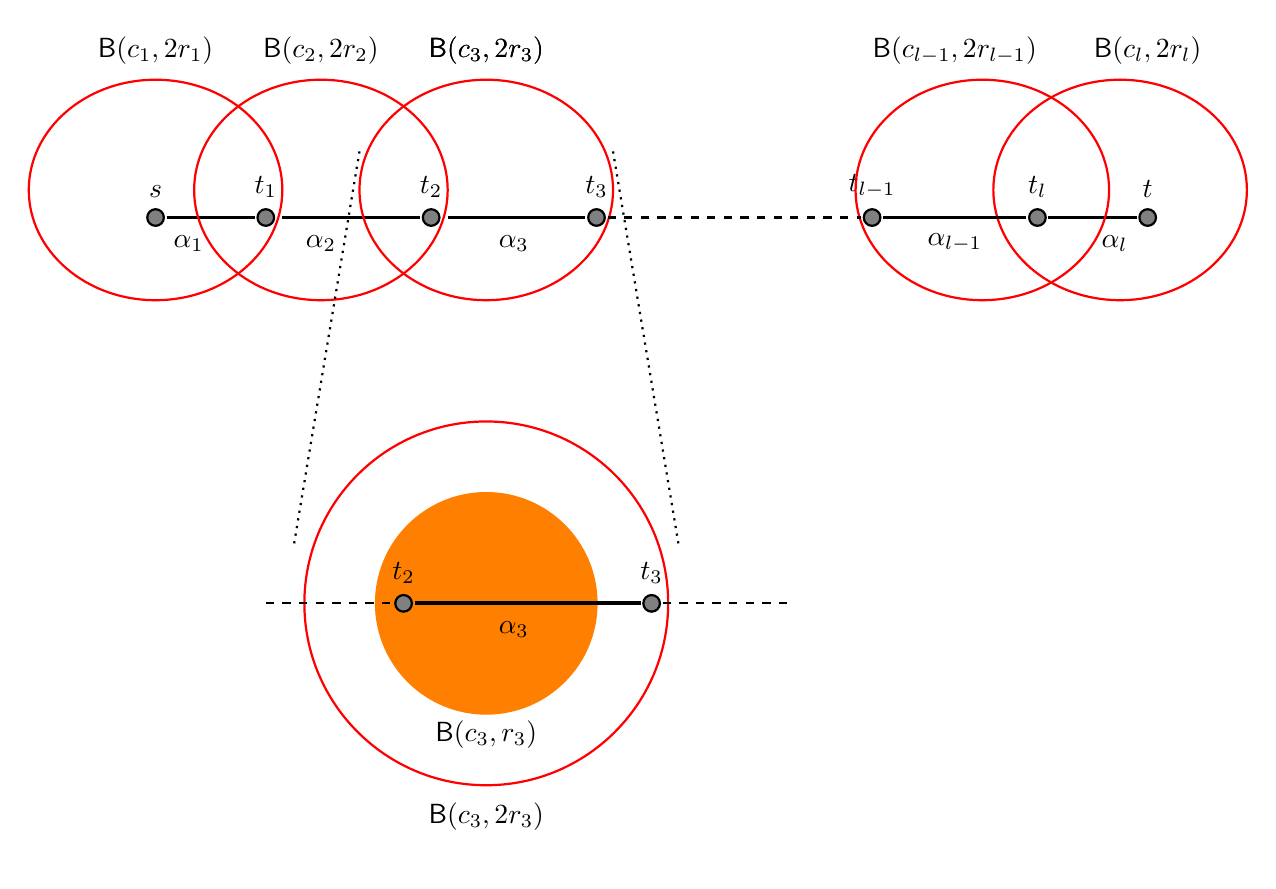
\begin{tikzpicture}[thick,scale=0.7]
	\draw (0, 0) node[circle, draw, fill=black!50, inner sep=0pt, minimum width=6pt, label = $s$] {};
	\draw (18, 0) node[circle, draw, fill=black!50, inner sep=0pt, minimum width=6pt,label = $t$] {};
	
	\draw (2, 0) node[circle, draw, fill=black!50, inner sep=0pt, minimum width=6pt,label = $t_1$] {};
	\draw [line width = 0.5mm] (0.2, 0) -- (1.8, 0);
	\draw (0.6, -1) node[red, label={$\alpha_1$}]{};
	\draw [red] (0, 0.5) ellipse (2.3 and 2);
	\draw (0, 2.4) node[red, label={$\ball(c_1, 2r_{1})$}]{};
	
	\draw (5, 0) node[circle, draw, fill=black!50, inner sep=0pt, minimum width=6pt,label = $t_2$] {};
	\draw [line width = 0.5mm] (2.3, 0) -- (4.8, 0);
	\draw (3, -1) node[red, label={$\alpha_2$}]{};
	\draw [red] (3, 0.5) ellipse (2.3 and 2);
	\draw (3, 2.4) node[red, label={$\ball(c_2, 2r_{2})$}]{};
	
	\draw (8, 0) node[circle, draw, fill=black!50, inner sep=0pt, minimum width=6pt,label = $t_3$] {};
	\draw [line width = 0.5mm] (5.3, 0) -- (7.8, 0);
	\draw (6.5, -1) node[red, label={$\alpha_3$}]{};
	\draw [red] (6, 0.5) ellipse (2.3 and 2);
	\draw (6, 2.4) node[red, label={$\ball(c_3, 2r_{3})$}]{};
	
	\draw[dotted] (3.7, 1.2) -- (2.5, -6);
	\draw[dotted] (8.3, 1.2) -- (9.5, -6);
	\draw [fill=orange,orange] (6, -7) ellipse (2 and 2);
	\draw (6, -10) node[red, label={$\ball(c_3, r_{3})$}]{};
	\draw (4.5, -7) node[circle, draw, fill=black!50, inner sep=0pt, minimum width=6pt,label = $t_2$] {};
	\draw (9, -7) node[circle, draw, fill=black!50, inner sep=0pt, minimum width=6pt,label = $t_3$] {};
	\draw [red] (6, -7) ellipse (3.3 and 3.3);
	\draw (6, -11.5) node[red, label={$\ball(c_3, 2r_{3})$}]{};
	\draw (6, 2.4) node[red, label={$\ball(c_3, 2r_{3})$}]{};
	\draw [line width = 0.5mm] (4.7, -7) -- (8.8, -7);
	\draw (6.5, -8) node[red, label={$\alpha_3$}]{};
	\draw [dashed] (2, -7) -- (4.3, -7);
	\draw [dashed] (9.2, -7) -- (11.5, -7);
	
	
	\draw (16, 0) node[circle, draw, fill=black!50, inner sep=0pt, minimum width=6pt,label = $t_l$] {};
	\draw [line width = 0.5mm] (17.8, 0) -- (16.2, 0);
	\draw (17.4, -1) node[red, label={$\alpha_l$}]{};
	\draw [red] (17.5, 0.5) ellipse (2.3 and 2);
	\draw (18, 2.4) node[red, label={$\ball(c_l, 2r_{l})$}]{};
	
	\draw (13, 0) node[circle, draw, fill=black!50, inner sep=0pt, minimum width=6pt,label = $t_{l-1}$] {};
	\draw [line width = 0.5mm] (15.8, 0) -- (13.2, 0);
	\draw (14.5, -1) node[red, label={$\alpha_{l-1}$}]{};
	\draw [red] (15, 0.5) ellipse (2.3 and 2);
	\draw (14.5, 2.4) node[red, label={$\ball(c_{l-1}, 2r_{l-1})$}]{};
	
	\draw [dashed] (8.2, 0) -- (12.8, 0); 
\end{tikzpicture}
	\end{center}
	\caption{A partitioning of the shortest path $\pi$ from $s$ to $t$ into subpaths $\alpha_1, \alpha_2, \ldots, \alpha_l$ by balls in $\clusters$. Note that in general $G[\ball(c_i, 2r_i)]$ does not necessarily contain the entire sub-path $\alpha_i$.}\label{path-partition}
\end{figure}

We prove the following simple properties of the subroutine.

\begin{observation}\label{different-balls}
	All balls in $\set{\ball(c_i, r_i)}_{1\leq i\leq l}$ are distinct.
\end{observation}
\begin{proof}
	Suppose otherwise that a ball is selected twice by \pathpart, namely $(c_i, r_i) = (c_j, r_j)$ for some $1\leq i<j\leq l$. Then, by the algorithm description we have $t_j\in \ball(c_j, 2r_j) = \ball(c_i, 2r_i)$, which contradicts the choice of $t_i$ which is the closest-to-$t$ vertex in $\ball(c_i, 2r_i)$ on $\pi$.
\end{proof}

\begin{observation}
For each $1\le i\le l$, the subpath $\alpha_i$ is entirely contained in the ball $\ball(c_i,4r_i)$.
\end{observation}
\begin{proof}
From the description of the subroutine, for each $1\le i\le l$, $s_i\in \ball(c_i, r_i)$ and $t_i\in \ball(c_i, 2r_i)$. Therefore, for every vertex $u\in \pi[s_i, t_i]$, by triangle inequality: $$\dist_{G}(c_i, u)\leq \dist_{G}(c_i, s_i) + \dist_{G}(s_i, t_i)\leq \dist_{G}(c_i, s_i) + \dist_G(c_i, s_i) + \dist_{G}(c_i, t_i)\leq 4r_i,$$
which implies that $u\in \ball(c_i, 4r_i)$.
\end{proof}

\begin{observation}\label{obs}
%Consider the moment when we have decomposed a shortest path $\pi$ as a concatenation of $\alpha_1, \alpha_2, \cdots, \alpha_l$, then we always have 
Let $R$ be the minimum radius of the balls in $\balls$. Then $l \leq |\pi|/R+1$. 
	%Plus, each path $\alpha_i$ lies within the induced subgraph $G[\ball(c_i, 4r_i)],\forall 1\leq i\leq l$.
\end{observation}
\begin{proof}
It suffices to show that, for each $1\leq i<l$, $|\alpha_i|\ge R$.
%By the algorithm description, each sub-path $\alpha_i$ is equal to $\pi[v, w]$ at some point during the iterative procedure. At the moment, the algorithm picked a ball $\ball(c, r)\in \clusters$ containing $v$, and then $w\in \pi(v, t]\cap \ball(c, 2r)$ is the closest vertex to $t$ on $\pi$ that lies in $\ball(c, 2r)$. 
From the algorithm, vertex $s_i$ belongs to the ball $\ball(c_i,r_i)$, and vertex $v_i$ is the last vertex on $\pi$ that lies in the ball $\ball(c_i,2 r_i)$, so if $t_i\neq t$ then $\dist_{G}(t_i,c_i)=2r_i$ must hold. Therefore, 
%As $i<l$, we have $w\neq t$. Then, as $w\in\ball(c, 2r)$ is the closest vertex on $\pi$ to $t$, it must be $w\in\ball^=(c, 2r)$. Then, by triangle inequality, we have:
$|\pi[s_i, t_i]|\geq \dist_{G}(c_i, t_i) - \dist_G(c_i, s_i)\geq 2r_i - r_i = r_i \geq R$.
\end{proof}


 
\paragraph{Level of balls.} Before we describe the algorithm for constructing the sets $\set{\pset_c}$, we first classify all clusters according to their sizes as follows.
Recall that we are initially given a set $\pset\subseteq V\times V$ of pairs in $G$.
For each integer $1\leq i\leq \ceil{1/\epsilon}$, we say that a ball $\ball(c, r)$ is \emph{at level $i$} iff $$n^{1-i\epsilon}/\sqrt{|\pset|}< |\ball(c, r)|\le n^{1-(i-1)\epsilon}/\sqrt{|\pset|}.$$
Denote by $\clusters_i$ the set of all level-$i$ balls in $\clusters$.
%define $$\clusters_i = \{\ball(c, r)\mid |\ball(c, r)|\in [n^{1-(i+1)\epsilon} / |P|^{1/2}, n^{1-i\epsilon}/|P|^{1/2}] \}\subseteq \clusters$$
We define the set of level-$0$ balls as $\clusters_0 = \{\ball(c, r)\mid |\ball(c, r)|> n/\sqrt{|\pset|}\}$, so $\balls=\clusters_0 \cup \clusters_1\cup\cdots\cup\clusters_{\ceil{1/\eps}}$. A ball from $\clusters$ is called \textbf{large} if it is in $\clusters_0$, and \textbf{small} otherwise. Here is a simple observation.
%Also, define parameters $K_i = \ceil{n^{(i+1)\epsilon}}$.

\iffalse
\paragraph{Phase 1: processing $\clusters_0$.} Take a random subset of vertices $S\subseteq V$ of size $\ceil{10|P|^{1/2}\log n}$. Since each ball $\ball(c, r)\in \clusters_0$ has size at least $n/|P|^{1/2}$, then with high probability, $S\cap \ball(c, r)\neq\emptyset$ for each $\ball(c, r)\in \clusters_0$. Define a path set: $$\Pi = \{\pi_{s, t}\mid s, t\in S, \dist_{G}(s, t) < 2D + 4\cdot 2^{10/\epsilon}D^{1-1/k}\}$$
For each $\ball(c, r)\in\clusters$, initialize a vertex set $U_c\leftarrow\emptyset$. 
\fi

\begin{observation}
For each $0\leq i\leq \ceil{1/\eps}$, $|\clusters_i|\leq O(n^{(i+1)\epsilon}\sqrt{|\pset|}/\epsilon)$.
\end{observation}
\begin{proof}
	By Lemma \ref{clustering}, $\sum_{\ball(c, r)\in\clusters_i}|\ball(c, r)|\leq \sum_{\ball(c, r)\in\clusters_i}|\ball(c, 4r)|\le O(n^{1+\eps}/\eps)$, and since each ball in $\bset_i$ has size at least $n^{1-i\epsilon} / \sqrt{|\pset|}$, $|\clusters_i|\leq O(n^{(i+1)\epsilon}\sqrt{|\pset|}/\epsilon)$.
\end{proof}


%\znote{some explanation}


\subsection{Step 1. Handling large balls}

We first take a uniformly random subset $S\subseteq V$ of size $\ceil{10\sqrt{|\pset|}\log n}$. Since each ball in $\clusters_0$ contains at least $n/\sqrt{|\pset|}$ vertices, with high probability, $S$ intersects all balls in $\balls_0$. 

We now proceed to iteratively construct the sets $\set{\pset_c}$ of pairs. Throughout, we maintain, for each  ball $\ball(c,r)\in \bset$, a set $\pset_c$ of pairs of vertices in $\ball(c,2r)$, and another set $U_c\subseteq S$ of vertices in $V$, which are initially empty sets. Intuitively, $U_c$ collects all vertices in $S$ whose distances from the ball center $c$ are already preserved by the spanner $H_D$ during the algorithm.

For every pair $s,t$ of vertices in $S$, we denote by $\pi_{s,t}$ an arbitrary shortest path connecting them in $G$, and we compute the set 
$$\Pi= \{\pi_{s, t}\mid s, t\in S, \text{ } \dist_{G}(s, t) < 2D + 4\cdot 2^{10/\epsilon}\cdot D^{1-1/k}\}.$$
%For each $\ball(c, r)\in\clusters$, initialize a vertex set $U_c\leftarrow\emptyset$. 

We then process all paths in $\Pi$ sequentially in an arbitrary order. For each path $\pi_{s, t}\in \Pi$, we first apply the subroutine \pathpart to it and the collection $\bset$ of balls, and obtain a partition $\pi_{s,t} = \alpha_1\circ\alpha_2\circ\cdots \circ\alpha_l$. 
For each $1\le i\le l$, we denote by $\ball(c_i, r_i)$ the ball that hosts the subpath $\alpha_i$.
If there exists a ball $\ball(c_i, r_i)$ such that $s, t\in U_{c_i}$, then we do nothing and move on to the next path in $\Pi$. Otherwise, for each $1\le  i\le l$, we add both vertices $s,t$ to the set $U_{c_i}$, and add the pair $(s_i, t_i)$ to the set $\pset_{c_i}$ of pairs.

\paragraph{Stretch analysis of Step 1.}
We make use of the following simple observation.
\begin{observation}\label{large-ball-size}
	At the end of Step 1, for each ball $\ball(c, r)\in \clusters$,  $|\pset_c|\leq |S| = \ceil{10|\pset|^{1/2}\log n}$.
\end{observation}
\begin{proof}
	By the algorithm description along with \Cref{different-balls}, every time a new pair is added to $\pset_c$, a new vertex from $S$ is also added to $U_c$. Since no more pair will be added to $\pset_{c}$ as long as $U_c$ contains all vertices of $S$, we get that $|\pset_c|\leq |U_c|\leq |S| = \ceil{10|\pset|^{1/2}\log n}$.
\end{proof}

%As the beginning of our stretch analysis, 
We now show in the following claims that, after the first step, all pairwise distances (in $G$) between vertices in $S$ are well-preserved in $H_D$. And as the set $S$ hits all balls in $\bset_0$ with high probability, the distance between any pair of vertices from $V(\balls_0)$ is also well-preserved.
% As $S$ hits every ball in $\bset_0$, this implies that the distance (in $G$) between every pair of vertices in $V(\bset_0)$ is well-preserved.

\begin{claim}\label{C0}
%During the enumeration of paths from $\Pi$, for any vertex $s\in S$ and ball $\ball(c, r)\in \clusters$, 
After a vertex $s\in S$ is added to the set $U_c$ for some $\ball(c,r)\in \bset$, the following holds:
	$$\dist_{H_D}(s, c)\leq \dist_G(s, c) + 49\cdot 2^{(30k-10)/\epsilon}\cdot D^{1-1/k}.$$
\end{claim}
\begin{proof}
Assume that the shortest path $\pi_{s,t}$ was being processed when $s$ was added to $U_c$, and that $\ball(c, r)$ was $\ball(c_i, r_i)$ under the notation of the subroutine \pathpart. From the algorithm, for each $1\leq j\leq l$, the pair $(s_j, t_j)$ was added to the collection $\pset_{c_j}$. From the construction of $H_D$, for each $1\leq j\leq l$, there exists a path $\phi_j$ in $H_D$ from $s_j$ to $t_j$, such that: 
	$$\begin{aligned}
	|\phi_j| \leq |\alpha_j| + 2^{30(k-1)/\epsilon}\cdot |\alpha_j|^{1-1/(k-1)} &\leq |\alpha_j| + 2^{30(k-1)/\epsilon}\cdot \left(4\cdot 2^{10/\epsilon}\cdot D^{1-1/k}\right)^{1-1/(k-1)}\\
	&\leq |\alpha_j| + 4\cdot 2^{(30k-20)/\epsilon}\cdot D^{1-2/k}
	\end{aligned}$$
	(we have used the fact that $|\alpha_j| < \dist_G(s_j,t_j)\le \dist_G(s_j,c_j)+ \dist_G(t_j,c_j)\le  4r_{j} \leq 4\cdot 2^{10/\epsilon}\cdot D^{1-1/k}$). Taking a summation over all indices $1\leq j\leq i$ and using  \Cref{obs}, we have:
	$$\begin{aligned}
	\dist_{H_D}(s, c_i)&\leq  \dist_{H_D}(c_i, t_i)+ \dist_{H_D}(s, t_i)\\
	&\leq 2\cdot 2^{10/\epsilon}\cdot D^{1-1/k} + \dist_G(s, t_i) + 48\cdot 2^{(30k-10)/\epsilon}\cdot D^{1-1/k}\\
	&\leq 2\cdot 2^{10/\epsilon}\cdot D^{1-1/k} + (\dist_G(s, c_i) + \dist_G(c_i, t_i)) + 48\cdot 2^{(30k-10)/\epsilon}\cdot D^{1-1/k}\\
	&\leq \dist_G(s, c_i) + 49\cdot 2^{(30k-10)/\epsilon} \cdot D^{1-1/k}.
	\end{aligned}$$
\end{proof}

\begin{claim}\label{C0-ineq}
	For any $s, t\in S$ such that $\dist_G(s, t) < 2D + 4\cdot 2^{10/\epsilon}\cdot D^{1-1/k}$, we have:
	$$\dist_{H_D}(s, t)\leq \dist_G(s, t) + 100 \cdot 2^{(30k-10)/\epsilon}\cdot D^{1-1/k}.$$
\end{claim}
\begin{proof}
For any such pair of vertices $s, t\in S$, consider the moment when the shortest path $\pi_{s, t}\in \Pi$ was processed and partitioned into subpaths $\alpha_1,\ldots,\alpha_l$. We distinguish between the following two cases.
	\begin{itemize}[leftmargin=*]
		\item Case 1. There existed an index $1\le i\le l$ such that $s, t\in U_{c_i}$ at the moment.
		
		In this case, from \Cref{C0}:
		$$\dist_{H_D}(s, c_i)\leq \dist_G(s, c_i) + 49\cdot 2^{(30k-10)/\epsilon} \cdot D^{1-1/k}\leq \dist_G(s, s_i) + 50\cdot 2^{(30k-10)/\epsilon} \cdot D^{1-1/k},$$
		$$\dist_{H_D}(c_i, t)\leq \dist_G(c_i, t) +49\cdot 2^{(30k-10)/\epsilon}\cdot D^{1-1/k}\leq \dist_G(s_i, t) + 50\cdot 2^{(30k-10)/\epsilon}\cdot D^{1-1/k}.$$
		Summing up these two inequalities finishes the proof.
		
		\item Case 2. There did not exist any $i$ such that $s, t\in U_{c_i}$ at the moment.
		
		In this case, for each $1\leq j\leq l$, the pair $(s_j, t_j)$ was added to the set $\pset_{c_j}$. Similar to the proof of \Cref{C0}, for each $1\leq j\leq l$, there exists a path $\phi_j$ in $H_D$ from $s_j$ to $t_j$, such that: 
		$$\begin{aligned}
		|\phi_j| \leq |\alpha_j| + 2^{30(k-1)/\epsilon}\cdot |\alpha_j|^{1-1/(k-1)} &\leq |\alpha_j| + 2^{30(k-1)/\epsilon}\cdot \left(4\cdot 2^{10/\epsilon}\cdot D^{1-1/k}\right)^{1-1/(k-1)}\\
		&\leq |\alpha_j| + 4\cdot 2^{(30k-20)/\epsilon}\cdot D^{1-2/k}.
		\end{aligned}$$
		Taking a summation for all indices $1\leq j\leq l$ and using \Cref{obs}, we get that:
		$$\dist_{H_D}(s, t) \leq \dist_G(s, t) + 48\cdot 2^{(30k-10)/\epsilon} \cdot D^{1-1/k}.$$
	\end{itemize}
\end{proof}




\subsection{Step 2. Handling small balls} 

We now process all pairs $(s,t)\in \pset$ with $D\le \dist_G(s, t) < 2D$ in an arbitrary order. Take any such pair $(s,t)$, and compute a shortest path $\pi_{s,t}$ between them in $G$. We then apply the subroutine \pathpart to it and the collection $\bset$ of balls, and obtain a partitioning $\pi_{s,t} = \alpha_1\circ\alpha_2\circ\cdots \circ\alpha_l$ together with the balls $\set{\ball(c_i, r_i)}_{1\le i\le l}$ that host them. However, as the number of pairs $(s,t)\in \pset$ with $D\le \dist_G(s, t) < 2D$ can be very large, we cannot afford to add the pair $(s_i,t_i)$ to set $\pset_{c_i}$ for all $1\le i\le l$ as in Step 1, and will instead carefully pick a subset of indices in $[1,l]$ to do so.


%Go over each demand pair $(s, t)\in P$ such that $\dist_G(s, t)\in [D, 2D)$ in an arbitrary order. In each round, a pair $(s, t)\in P$ is enumerated, and let $\pi$ be a shortest path between $s, t$. Apply the path partition subroutine to obtain sub-paths $\alpha_1, \alpha_2, \cdots, \alpha_l$ and balls $\ball(c_1, r_{c_1}), \ball(c_2, r_{c_2}), \cdots, \ball(c_l, r_{c_l})$. 



%For the rest of this round, we will be adding some pairs $(s_i, t_i)$ to $P_{c_i}$. During the process, each index $i\in [1, l]$ has two fields:
\iffalse
\begin{itemize}
	\item \textbf{Marked} or \textbf{unmarked}
	
	Index $i$ is marked if $(s_i, t_i)$ has already been added to $P_{c_i}$; otherwise $i$ is unmarked.
	
	\item \textbf{Ranks}
	
	Then level of index $i$ is equal to $\rk$ if $\ball(r_i, c_{r_i})\in\clusters_\rk$.
\end{itemize}
\fi

We will now describe how to choose these indices. This is again done via an iterative process. Throughout, we will gradually construct a binary tree $\tree$, which initially contains a single node, which is the root of $\tree$. 
Each node of the tree is labeled by a subinterval of $[1, l]$. Initially, the root of $\tree$ is labeled with $[1, l]$. %The tree $\tree$ is grown downward by a repetitive procedure.
Each index $i\in [1,l]$ is either marked \textbf{active} or \textbf{inactive}. Initially, all indices are inactive. The algorithm continues to be executed unless for each leaf of the tree $\tree$, all indices in its associated interval are active. Over the course of the algorithm, whenever we mark some index $i$ active, we will simultaneously add the pair $(s_i,t_i)$ to the set $\pset_{c_{i}}$.
We say that an index $i\in [1,l]$ is \textbf{at level $j$} iff its corresponding ball $\ball(c_i,r_i)$ is at level $j$ (that is, if $n^{1-j\epsilon}/\sqrt{|\pset|}< |\ball(c_i, r_i)|\le n^{1-(j-1)\epsilon}/\sqrt{|\pset|}$).

As a pre-processing step, we first focus on level-$0$ indices (if there are none of them, then we skip the pre-processing). Let $i_1, i_2$ be the smallest and the largest level-$0$ indices, respectively. We add two new nodes to the tree $\tree$, connecting each of them to the root by an edge. One of the new nodes is labeled by interval $[1, i_1-1]$, and the other node is labeled by interval $[i_2+1, l]$. So now the levels of indices on $[1, i_1-1]$ and $[i_2+1, l]$ are at least $1$. Here we do not modify the active/inactive status of the indices.

%The repetitive procedure is as follows. At the root of $\tree$ we first perform one step of preprocessing. If there is a sub-path $\alpha_i$ with level $0$, then let $i_1, i_2$ be the smallest and the largest indices such that $i_1, i_2$ have level $0$. Then, grow two children $N_1, N_2$ associated with interval $[1, i_1]$ and $[i_2, l]$, respectively. 

%For the rest, each time pick an arbitrary node $N$ which is currently is a leaf containing some unmarked indices; if such node $N$ does not exist anymore, the construction of $\tree$ is complete. Denote by $[i', i'']$ the interval associated with $N$.

%We the process level-$i$ indices sequentially for $i=1,\ldots,\ceil{1/\eps}$.

We now describe an iteration. We take an arbitrary leaf of the tree $\tree$ that whose associated interval contains an inactive index, and denote by $I$ the interval associated with this leaf node. We can assume that all levels of $I$ are at least $1$.
For each $1\le L\le \ceil{1/\eps}$, let $i^L_1 < i^L_2 <\cdots < i^L_{p(L)}$ be all level-$L$ indices in the interval $I$ (so the number of level-$L$ indices in $I$ is $p(L)$); we will \textbf{ignore the superscript $L$} if it is clear from context. Consider the corresponding balls $\set{\ball(c_{i^L_a}, r_{i^L_a})}$ that host them. We say that a pair $\left(\ball(c_{i^L_a}, r_{i^L_a}), \ball(c_{i^L_b}, r_{i^L_b})\right)$ of balls is \textbf{tight}, iff 
$$\dist_{H_D}(c_{i^L_a}, c_{i^L_b}) \le \dist_G(c_{i^L_a}, c_{i^L_b}) + \left(3\cdot 2^{(30k-20)/\epsilon} + 10\cdot 2^{10/\epsilon}\right)\cdot D^{1-1/k}.$$
and we denote by $q(L)$ the number of pairs of balls in $\set{\ball(c_{i^L_a}, r_{i^L_a})}$ which are not tight. In addition, we define $\beta(L)=\ceil{n^{(L+1)\epsilon}}$.

We will distinguish between the following two cases.

\begin{comment}
	\iffalse
	We will classify all unmarked levels into two different types. For any level-$L$ such that interval $[i', i'']$ contains some unmarked indices of level $L$, let $x\leq i_1 < i_2 <\cdots < i_p\leq y$ be all such indices.  Let $q$ be the total number of pairs of balls $(\ball(c_{i_a}, r_{c_{i_a}}), \ball(c_{i_b}, r_{c_{i_b}})), 1\leq a<b\leq p$ such that:
	$$\dist_{H_D}(c_{i_a}, c_{i_b}) > \dist_G(c_{i_a}, c_{i_b}) + \left(3\cdot 2^{(30k-20)/\epsilon} + 10\cdot 2^{10/\epsilon}\right)D^{1-1/k}$$
	To classify this level $\rk$ as Type (A) or Type (B), it depends on the comparison between $p$ and $q$.
	\begin{enumerate}[(A)]
		\item $p \leq \max\{4\cdot \ceil{n^{(\rk+1)\epsilon}}, 8q /\ceil{n^{(\rk+1)\epsilon}} \}$.
		
		\item $p > \max\{4\cdot \ceil{n^{(\rk+1)\epsilon}}, 8q /\ceil{n^{(\rk+1)\epsilon}} \}$.
	\end{enumerate}
	
	The algorithm takes the following branching depending on types of levels within $[i', i'']$.
	\fi
\end{comment}

\paragraph{Case 1. For all $1\le L\le \ceil{1/\eps}$, $p(L) \leq \max\{4\beta(L), 8q(L)/\beta(L) \}$.}
In this case, we activate all indices $i\in I$ (and along with it add the corresponding pair $(s_{i}, t_{i})$ to the set $\pset_{c_{i}}$ and then update $H_D$ accordingly), and continue to the next iteration. We do not modify the tree $\tree$ in this iteration. Note that, after this iteration, the associated interval of the leaf that we processed in this iteration no longer contains any inactive indices, so it will remain a leaf in $\tree$ forever.

\paragraph{Case 2. There exists some $1\le L\le \ceil{1/\eps}$, such that $p(L) > \max\{4\beta(L), 8q(L)/\beta(L) \}$.}
In this case, 
%for each $a\in [1, \beta(L)]\cup [p(L)-\beta(L)+1, p(L)]$, 
we activate the $\beta(L)$ smallest and $\beta(L)$ largest level-$L$ indices in $I$ (and along with it add the corresponding pair $(s_{i}, t_{i})$ to the set $\pset_{c_{i}}$ and then update $H_D$ accordingly).

In order to describe the modification of $\tree$ in this iteration, we need the following lemma.

%To proceed with the rest of this iteration of growing $\tree$, we need to first state an important property.
\begin{lemma}
	There exists three level-$L$ indices $i_x, i_y, i_z\in I$ such that:
	\begin{enumerate}[(i)]
		\item $1\leq x\leq \beta(L)$;
		\item $p(L)-\beta(L) < y\leq p(L)$;
		\item $\beta(L) < z\leq p(L)-\beta(L)$;
		\item the pair $\left(\ball(c_{i_x}, r_{i_x}),\ball(c_{i_z}, r_{i_z})\right)$ and the pair $\left(\ball(c_{i_y}, r_{i_y}),\ball(c_{i_z}, r_{i_z})\right)$ of balls are both tight.
	\end{enumerate}
\end{lemma}
\begin{proof}
	Assume for contradiction that there do not exist such three indices. Consider now any pair $a,b$ of indices such that $1\le a\le \beta(L)$ and $\beta(L) < b \leq p(L) - \beta(L)$. From our assumption, for at least one pair of indices $(i^L_a,i^L_{b})$ and $(i^L_b,i^L_{p(L)+1-a})$, their corresponding balls are not tight.
	This implies that $q(L)\geq (p(L) - 2\beta(L))\cdot\beta(L)$. Then either $p(L)<4\beta(L)$ holds, or $q(L)\geq p(L)\cdot \beta(L) / 8$ holds, a contradiction of the initial assumption of Case 2.
	\iffalse
	Suppose the statement does not hold. Then, for any triple of indices: 
		$$x\in [1, K_\rk], y = p+1 - x\in [p-K_\rk+1, p], z\in [K_\rk+1, p-K_\rk]$$
		We know that at least one of the following two inequalities hold:
		$$\dist_{H_D}(c_{i_{x}}, c_{i_{z}})> \dist_G(c_{i_{x}}, c_{i_{z}}) + \left(3\cdot 2^{(30k-20)/\epsilon} + 10\cdot 2^{10/\epsilon}\right)D^{1-1/k}$$
		$$\dist_{H_D}(c_{i_{z}}, c_{i_{y}})> \dist_G(c_{i_{z}}, c_{i_{y}}) + \left(3\cdot 2^{(30k-20)/\epsilon} + 10\cdot 2^{10/\epsilon}\right) D^{1-1/k}$$
		
		Hence, for any $x\in [1, K_\rk], z\in [K_\rk+1, p-K_\rk]$, either the pair $(\ball(c_{i_{x}}, r_{c_{i_{x}}}), \ball(c_{i_{z}}, r_{c_{i_{z}}}))$ should contribute to the counting of $q$, or $(\ball(c_{i_{y}}, r_{c_{i_{y}}}), \ball(c_{i_{z}}, r_{c_{i_{z}}}))$ should do so. Therefore, $q\geq (p - 2K_\rk)\cdot K_\rk \geq p\cdot K_\rk / 8$, which is a contradiction of the definition of Type (B).
	\fi
\end{proof}

To complete this iteration, we pick indices $i_x, i_y, i_z$ as in the above lemma. We then add two new nodes to the tree $\tree$ (together with an edge connecting to the leaf) as the child nodes of this leaf. 
Denote $I=[i',i'']$, and we label the child nodes with intervals $[i', i_{x}]$ and $[i_{y}, i'']$, respectively. This completes the description of an iteration. See Figure \ref{bridge} for an illustration.


\begin{figure}[h]
	\begin{center}
		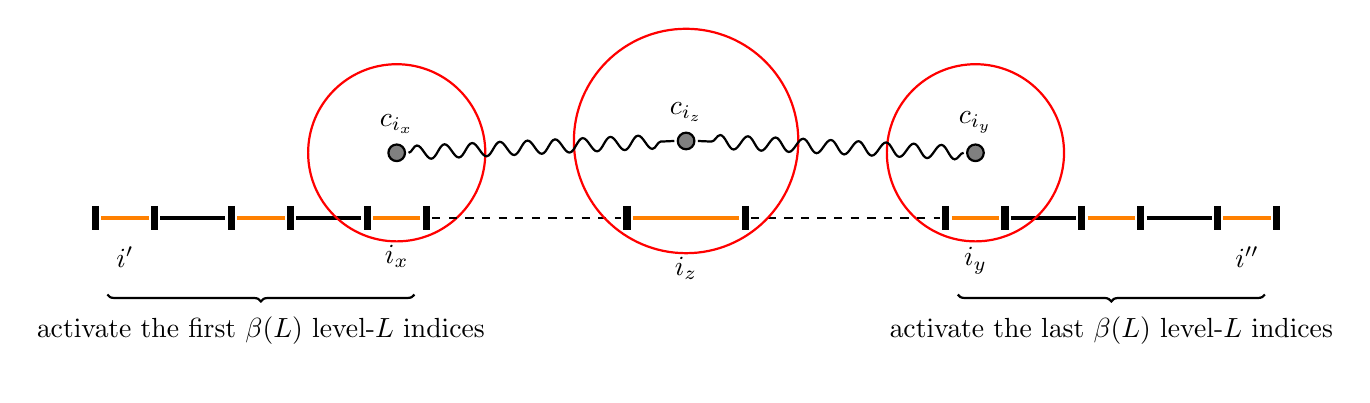
\begin{tikzpicture}[thick,scale=0.75]
	\draw [line width = .9mm] (0, 0.2) -- (0, -0.2);
	\draw [line width = .9mm] (1, 0.2) -- (1, -0.2);
	\draw [line width = 0.5mm, color=orange] (0.1, 0) -- (0.9, 0);
	\draw (0.5, -1.2) node[red, label={$i'$}]{};
	
	\draw [line width = 0.5mm] (1.1, 0) -- (2.2, 0);
	
	\draw [line width = .9mm] (2.3, 0.2) -- (2.3, -0.2);
	\draw [line width = .9mm] (3.3, 0.2) -- (3.3, -0.2);
	\draw [line width = 0.5mm, color=orange] (2.4, 0) -- (3.2, 0);
	%\draw (2.8, -1.2) node[red, label={$x+1$}]{};
	
	\draw [line width = 0.5mm] (3.4, 0) -- (4.5, 0);
	
	\draw [line width = .9mm] (4.6, 0.2) -- (4.6, -0.2);
	\draw [line width = .9mm] (5.6, 0.2) -- (5.6, -0.2);
	\draw [line width = 0.5mm, color=orange] (4.7, 0) -- (5.5, 0);
	\draw (5.1, -1.2) node[red, label={$i_{x}$}]{};
	\draw [red] (5.1, 1.1) ellipse (1.5 and 1.5);
	\draw (5.1, 1.1) node[circle, draw, fill=black!50, inner sep=0pt, minimum width=6pt, label = $c_{i_{x}}$] {};
	
	\draw [decorate,
	decoration = {brace}] (5.4,-1.3) -- (0.2,-1.3);
	\draw (2.8, -2.5) node[label={activate the first $\beta(L)$ level-$L$ indices}]{};
	
	\draw [line width = .9mm] (20, 0.2) -- (20, -0.2);
	\draw [line width = .9mm] (19, 0.2) -- (19, -0.2);
	\draw [line width = 0.5mm, color=orange] (19.1, 0) -- (19.9, 0);
	\draw (19.5, -1.2) node[red, label={$i''$}]{};
	
	\draw [line width = 0.5mm] (17.8, 0) -- (18.9, 0);
	
	\draw [line width = .9mm] (17.7, 0.2) -- (17.7, -0.2);
	\draw [line width = .9mm] (16.7, 0.2) -- (16.7, -0.2);
	\draw [line width = 0.5mm, color=orange] (16.8, 0) -- (17.6, 0);
	%\draw (17.2, -1.2) node[red, label={$y-1$}]{};
	
	\draw [line width = 0.5mm] (15.5, 0) -- (16.6, 0);
	
	\draw [line width = .9mm] (15.4, 0.2) -- (15.4, -0.2);
	\draw [line width = .9mm] (14.4, 0.2) -- (14.4, -0.2);
	\draw [line width = 0.5mm, color=orange] (14.5, 0) -- (15.3, 0);
	\draw (14.9, -1.3) node[red, label={$i_{y}$}]{};
	\draw [red] (14.9, 1.1) ellipse (1.5 and 1.5);
	\draw (14.9, 1.1) node[circle, draw, fill=black!50, inner sep=0pt, minimum width=6pt, label = $c_{i_{y}}$] {};
	
	\draw [decorate,
	decoration = {brace}] (19.8,-1.3) -- (14.6,-1.3);
	\draw (17.2, -2.5) node[label={activate the last $\beta(L)$ level-$L$ indices}]{};
	
	\draw [dashed] (5.7, 0) -- (8.9, 0);
	\draw [line width = .9mm] (9, 0.2) -- (9, -0.2);
	\draw [line width = .9mm] (11, 0.2) -- (11, -0.2);
	\draw [line width = 0.5mm, color=orange] (9.1, 0) -- (10.9, 0);
	\draw (10, -1.4) node[red, label={$i_{z}$}]{};
	\draw [dashed] (11.1, 0) -- (14.3, 0);

	\draw [red] (10, 1.3) ellipse (1.9 and 1.9);
	\draw (10, 1.3) node[circle, draw, fill=black!50, inner sep=0pt, minimum width=6pt, label = $c_{i_{z}}$] {};
	
	\draw [style={decorate, decoration=snake}] (5.3, 1.1) -- (9.8, 1.3);
	\draw [style={decorate, decoration=snake}] (14.7, 1.1) -- (10.2, 1.3);
\end{tikzpicture}
	\end{center}
	\caption{The distances between $c_{i_{x}}, c_{i_{z}}$ and $c_{i_{y}}, c_{i_{z}}$ are approximately preserved in $H$; the orange segments correspond to level-$L$ indices; a prefix and a suffix of level-$L$ indices are activated in this iteration.}\label{bridge}
\end{figure}

%\subsection{Stretch analysis}

\iffalse
The following simple observation is the key to our analysis.
\begin{lemma}\label{obs0}
	Consider the moment when we have decomposed a shortest path $\pi$ as a concatenation of $\alpha_1, \alpha_2, \cdots, \alpha_l$, then we always have $l \leq \ceil{\frac{|\pi|}{D^{1-1/k}}}$. 
	%Plus, each path $\alpha_i$ lies within the induced subgraph $G[\ball(c_i, 4r_i)],\forall 1\leq i\leq l$.
\end{lemma}
\begin{proof}
	It suffices to show that each sub-path $\alpha_i, \forall 1\leq i<l$ has length at least $D^{1 - 1/k}$. By the algorithm description, each sub-path $\alpha_i$ is equal to $\pi[v, w]$ at some point during the iterative procedure. At the moment, the algorithm picked a ball $\ball(c, r)\in \clusters$ containing $v$, and then $w\in \pi(v, t]\cap \ball(c, 2r)$ is the closest vertex to $t$ on $\pi$ that lies in $\ball(c, 2r)$. 
	
	As $i<l$, we have $w\neq t$. Then, as $w\in\ball(c, 2r)$ is the closest vertex on $\pi$ to $t$, it must be $w\in\ball^=(c, 2r)$. Then, by triangle inequality, we have:
	$$|\pi[v, w]|\geq \dist_{G}(c, w) - \dist_G(c, v)\geq 2r - r = r \geq D^{1-1/k}$$
\end{proof}
\fi


\paragraph{Stretch analysis of Step 2.}
Consider any pair $(s, t)\in \pset$ such that $D\le \dist_G(s, t) < 2D$. Let $\pi$ be the shortest path connecting $s$ to $t$ that was processed in Step 2. We start by showing that, in this iteration, the depth of the tree $\tree$ that we construct is small. 

\begin{observation}
At the end of the iteration of processing $\pi$, $\tree$ has depth at most $\ceil{1/\eps}+1$.
\end{observation}
\begin{proof}
The pre-processing step can increase the depth by at most one. From the algorithm description, it is easy to observe that, as we walk down in any root-to-leaf path in $\tree$, in each step, the number of levels with inactive indices decreases by one. Hence, the observation follows.
%For the rest we only consider general steps that take the branching (1)(2). Consider any iteration where the algorithm picked a node $N$ which was a leaf containing some unmarked indices back then. If the algorithm took branch (1), then all indices from $[i', i'']$ would be marked immediately, and node $N$ would stay a leaf for the rest. If the algorithm took branch (2), then by the algorithm description, all indices with level $\rk$ within intervals $[i', i_{x}]$ and $[i_{y}, i'']$ are marked, hence the number of levels of unmarked indices in children $N_1, N_2$ decreases by at least one. Since the total number of levels is $\ceil{1/\eps}$, the maximum depth of $\tree$ in the end is at most $\ceil{1/\eps} + 1$.
\end{proof}

We are now ready to analyze the stretch (in $H_D$) of pairs in $\pset$.

\begin{lemma}
\label{lem: step 2}
For every pair $(s, t)\in \pset$, $\dist_{H_D}(s, t)\leq \dist_G(s, t) + 2^{30k/\epsilon}\cdot D^{1-1/k}$.
\end{lemma}
\begin{proof}
	We will utilize the tree structure of $\tree$. Focus on the time when the construction of $\tree$ was completed. For any tree node $N$, its \emph{height} is defined to be the maximum depth of the subtree of $\tree$ rooted at $N$. We first prove the following claim.
	
	\begin{claim}
	\label{clm: stretch by depth}
		For each non-root tree node $N$ with height $h$ and associated interval $[i', i'']$,
		$$\dist_{H_D}(c_{i'}, c_{i''})\leq \dist_G(c_{i'}, c_{i''}) + 30\cdot (2^{h+1}-1)\cdot 2^{(30k-20)/\epsilon}\cdot D^{1-1/k}.$$
	\end{claim}
	\begin{proof}[Proof of \Cref{clm: stretch by depth}]		
%	\znote{$i,i''$.}	
	We prove the claim by induction on $h$. The base case is when $h = 0$ and $N$ is a leaf in $\tree$. From the algorithm, for each $i\in [i', i'']$, the pair $(s_i, t_i)$ is added into the set $\pset_{c_i}$. Similar to the proof of \Cref{C0}, for each $i'\leq i\leq i''$, there exists a path $\phi_i$ in $H_D$, such that 
		$$\begin{aligned}
			|\phi_j| \leq |\alpha_j| + 2^{30(k-1)/\epsilon}\cdot |\alpha_j|^{1-1/(k-1)} &\leq |\alpha_j| + 2^{30(k-1)/\epsilon}\cdot \left(4\cdot 2^{10/\epsilon}\cdot D^{1-1/k}\right)^{1-1/(k-1)}\\
			&\leq |\alpha_j| + 4\cdot 2^{(30k-20)/\epsilon}\cdot D^{1-2/k}.
		\end{aligned}$$
		Taking a summation and using \Cref{obs} (which implies that $l<3D^{1/k}$),
		$$\dist_{H_D}(s_{i'}, t_{i''})\leq \dist_G(s_{i'}, t_{i''}) + 12\cdot 2^{(30k-20)/\epsilon}\cdot D^{1-1/k}.$$
		By triangle inequality, we have:
		$$\dist_{H_D}(s_{i'}, t_{i''})\geq \dist_{H_D}(c_{i'}, c_{i''}) - \dist_{H_D}(c_{i'}, s_{i'}) - \dist_{H_D}(c_{i''}, t_{i''})\geq \dist_{H_D}(c_{i'}, c_{i''}) - 3\cdot 2^{10/\epsilon}D^{1-1/k},$$
		$$\dist_G(s_{i'}, t_{i''})\leq \dist_G(c_{i'}, c_{i''}) + \dist_G(c_{i'}, s_{i'}) + \dist_G(c_{i''}, t_{i''})\leq \dist_G(c_{i'}, c_{i''}) + 3\cdot 2^{10/\epsilon}D^{1-1/k}.$$
		Combining all three inequalities, we have:
		$$\begin{aligned}
			\dist_{H_D}(c_{i'}, c_{i''})&\leq \dist_G(c_{i'}, c_{i''}) + \left(12\cdot 2^{(30k-20)/\epsilon} + 6\cdot 2^{10/\epsilon}\right)\cdot D^{1-1/k}\\
			&< \dist_G(c_{i'}, c_{i''}) + 30\cdot 2^{(30k-20)/\epsilon}\cdot D^{1-1/k}.
		\end{aligned}$$
		
		Assume now that the claim is true for $1,\ldots,h-1$. Consider a node $N$ at height $h$ with two children $N_1, N_2$ associated with intervals $[i', i_{x}]$ and $[i_{y}, i'']$ respectively. By inductive hypothesis, we have:
		$$\dist_{H}(c_{i'}, c_{i_{x}})\leq \dist_G(c_{i'}, c_{i_{x}}) + 30\cdot (2^{h}-1)\cdot 2^{(30k-20)/\epsilon}\cdot D^{1-1/k},$$
		$$\dist_{H}(c_{i''}, c_{i_{y}})\leq \dist_G(c_{i''}, c_{i_{y}}) + 30\cdot (2^{h}-1)\cdot 2^{(30k-20)/\epsilon}\cdot D^{1-1/k}.$$
		From the algorithm, the node $N$ may only grow two children $N_1$ and $N_2$ in Case 2, and in this case there exists an index $i_z$ such that the pairs $(\ball(c_{i_x}, r_{i_x}),\ball(c_{i_z}, r_{i_z}))$ and $(\ball(c_{i_y}, r_{i_y}),\ball(c_{i_z}, r_{i_z}))$ of balls are both tight. In other words,
		\[\dist_{H_D}(c_{i_{x}}, c_{i_{z}})\leq \dist_G(c_{i_{x}}, c_{i_{z}}) + \left(3\cdot 2^{(30k-20)/\epsilon} + 10\cdot 2^{10/\epsilon}\right)D^{1-1/k},\]
		\[\dist_{H_D}(c_{i_{z}}, c_{i_{y}})\leq \dist_G(c_{i_{z}}, c_{i_{y}}) + \left(3\cdot 2^{(30k-20)/\epsilon} + 10\cdot 2^{10/\epsilon}\right)D^{1-1/k}.\]
		The sum of the left-hand sides of the above four inequalities is at least $\dist_{H_D}(c_{i'}, c_{i''})$, from triangle inequality. For their right-hand sides, notice that: 
		\[\begin{aligned}
			\dist_G(c_{i'}, c_{i_{x}}) + \dist_G(c_{i_{x}}, c_{i_{z}})&\leq (\dist_G(s_{i'}, s_{i_{x}}) + \dist_G(c_{i'}, s_{i'}) + \dist_G(c_{i_{x}}, s_{i_{x}}))\\
			& +(\dist_G(s_{i_{x}}, s_{i_{z}}) + \dist_G(c_{i_{x}}, s_{i_{x}}) + \dist_G(c_{i_{z}}, s_{i_{z}}))\\
			&\leq \dist_G(s_{i'}, s_{i_{z}}) + 4\cdot 2^{10/\epsilon}\cdot D^{1-1/k}\\
			&\leq \dist_G(c_{i'}, c_{i_{z}}) + 6\cdot 2^{10/\epsilon}\cdot D^{1-1/k}.
		\end{aligned}
		\]
		Symmetrically, we also have $\dist_G(c_{i''}, c_{i_{y}}) + \dist_G(c_{i_{y}}, c_{i_{z}})\leq \dist_G(c_{i''}, c_{i_{z}}) + 6\cdot 2^{10/\epsilon}\cdot D^{1-1/k}$.
		
		Note that
		$\dist_G(c_{i'}, c_{i_{z}}) + \dist_G(c_{i''}, c_{i_{z}})\leq \dist_G(c_{i'}, c_{i''}) + 2\cdot 2^{10/\epsilon}\cdot D^{1-1/k}$ (again by triangle inequality). Altogether, we get that:
		$$\dist_{H_D}(c_{i'}, c_{i''})\leq \dist_G(c_{i'}, c_{i''}) + 30\cdot (2^{h+1}-1)\cdot 2^{(30k-20)/\epsilon}\cdot D^{1-1/k}.$$
	\end{proof}

	Lastly, we consider the root $N_0$ of $\tree$. Recall that it is associated with the interval $[1,l]$. 
	If there are no level-$0$ indices in $[1, l]$, then \Cref{clm: stretch by depth} already implies \Cref{lem: step 2}. We assume from now on that there are level-$0$ indices in $[1, l]$. From the algorithm, in the pre-processing step, $N_0$ grows two children $N_1, N_2$ associated with intervals $[1, i_1-1]$ and $[i_2+1, l]$, respectively, such that $i_1, i_2$ are the smallest and the largest level-$0$ indices. By definition of $S$, there exists $v_1, v_2$ such that $v_1\in (\ball(c_{i_1}, r_{i_1})\cap S), v_2\in (\ball(c_{i_2}, r_{i_2})\cap S)$. Notice that $\dist_G(v_1, v_2)\leq \dist_G(s_{i_1}, s_{i_2}) + 4\cdot 2^{10/\epsilon}\cdot D^{1-1/k} < 2D + 4\cdot 2^{10/\epsilon}\cdot D^{1-1/k} $. Then, from \Cref{C0-ineq}, we have:
	$$\dist_{H_D}(v_1, v_2)\leq \dist_G(v_1, v_2) + 100\cdot 2^{(30k-10)/\epsilon} D^{1-1/k}.$$
	
	Suppose $N_1, N_2$ have height $h_1, h_2\leq \ceil{1/\eps}$ respectively. By \Cref{clm: stretch by depth},
	$$\dist_{H_D}(c_1, c_{i_1-1})\leq \dist_G(c_1, c_{i_1-1}) + 30\cdot (2^{h_1+1}-1)\cdot 2^{(30k-20)/\epsilon}\cdot D^{1-1/k},$$
	$$\dist_{H_D}(c_l, c_{i_2+1})\leq \dist_G(c_l, c_{i_2+1}) + 30\cdot (2^{h_2+1}-1)\cdot 2^{(30k-20)/\epsilon}\cdot D^{1-1/k}.$$
%
Taking a summation of the left-hand sides of the above three inequalities:
	\[\begin{aligned}
		&\dist_{H_D}(c_1, c_{i_1-1}) + \dist_{H_D}(c_l, c_{i_2+1}) + \dist_{H_D}(v_1, v_2)\\
		& \geq \dist_{H_D}(c_1, c_{i_1-1}) + \dist_{H_D}(c_l, c_{i_2+1}) + \dist_{H_D}(c_{i_1}, c_{i_2}) - 2\cdot 2^{10/\epsilon}\cdot D^{1-1/k}\\
		&\geq \dist_{H_D}(c_1, c_l) - 8\cdot 2^{10/\epsilon}\cdot D^{1-1/k}\\
		&\geq \dist_{H_D}(s, t) - 11\cdot 2^{10/\epsilon} D^{1-1/k}.
	\end{aligned}\]
%
Taking a summation of their right-hand sides (ignoring the tails for now):
	\[\begin{aligned}
		\dist_G(c_1, c_{i_1-1}) + \dist_G(c_l, c_{i_2+1}) + \dist_G(v_1, v_2) & \leq \dist_G(s, s_{i_1-1}) + (\dist_G(s, c_1) + \dist_G(c_{i_1-1}, s_{i_1}))\\
		&+\dist_G(t, s_{i_2+1}) + (\dist_G(t, c_l) + \dist_G(s_{i_2+1}, c_{i_2}))\\
		&+ \dist_G(s_{i_1}, s_{i_2}) + (\dist_G(v_1, s_{i_1}) + \dist_G(v_2, s_{i_2}))\\
		&\leq \dist_G(s, t) + 9\cdot 2^{10/\epsilon}\cdot D^{1-1/k}.
\end{aligned} \]
%
Altogether, $\dist_{H_D}(s, t)\leq \dist_G(s, t) + 200\cdot 2^{(30k-10)/\epsilon}D^{1-1/k} < \dist_G(s, t) + 2^{30k/\epsilon}D^{1-1/k}$.
%Finally, if $[1, l]$ does not contain any level-$0$ indices, then we can prove the above inequality in a similar manner based on the inductive claim.
\end{proof}

\subsection{Size analysis}

In this subsection, we complete the proof of \Cref{pairwise-sublinear} by showing that the spanner $H$ constructed by the algorithm in this section satisfies the desired size bound. We start by proving the following claim.

\begin{claim}
\label{clm: pairs added}
In the end, for each level $1\leq i\leq \ceil{1/\eps}$, $\sum_{\ball(c, r)\in \clusters_i}|\pset_c|\leq O(\frac{1}{\epsilon^2}2^{\ceil{1/\epsilon}}n^{(i+1)\epsilon}|\pset|\log n)$.
\end{claim}
\begin{proof}
%For $i = 0$, note that the algorithm never increases $|\pset_c|$ when $\ball(c, r)\in \clusters_0$ during Step 2, so by \Cref{large-ball-size}, $|\pset_c|\leq O(|\pset|^{1/2}\log n)$. Since $|\clusters_0|\leq O(n^\epsilon |\pset|^{1/2}/\epsilon)$, the inequality holds.

By \Cref{large-ball-size}, all sets $\pset_c$ have size $O(|\pset|^{1/2}\log n)$ before Step 2 begins. Hence, at the time when Step 1 finishes, we have $\sum_{\ball(c, r)\in \clusters_i}|\pset_c|\leq O(\frac{1}{\epsilon}n^{(i+1)\epsilon}|\pset|\log n)$. So, we only need to analyze how much $|\pset_c|$ has increased during Step 2. 
%Throughout Phase 2, let $\Phi_i$ be the total number of pairs of balls $(\ball(c_1, r_{c_1}), \ball(c_2, r_{c_2}))\in \clusters_i\times\clusters_i$, such that: $$\dist_{H_D}(c_1, c_2) > \dist_G(c_{1}, c_{2}) + \left(3\cdot 2^{(30k-20)/\epsilon} + 10\cdot 2^{10/\epsilon}\right)D^{1-1/k}$$

Define $\Phi_i$ to be the number of  pairs of level-$i$ balls that are not tight. So, at the beginning of Step 2, we have $\Phi_i\le |\clusters_i|^2\leq O(n^{2(i+1)\epsilon}|\pset|/\epsilon^2)$.

Consider the iteration in Step 2 when some pair $(s,t)\in \pset$ was being processed, and let $\tree$ be the binary tree constructed in that iteration. Let $N$ be a node of $\tree$. If the algorithm added more than $4\beta(i)$ pairs to $\bigcup_{\ball(c, r)\in\clusters_i}\pset_c$ in the round that $N$ was processed, then it must be through Case 1 and $N$ would remain a leaf in $\tree$ till the end. Put in other way, at most $4\beta(i)$ pairs were added to the collections $\bigcup_{\ball(c, r)\in\clusters_i}\pset_c$ in processing every non-leaf node in $\tree$.
Consider now a leaf node $N$ of $\tree$.
%Suppose $i_1 < i_2<\cdots< i_{p}$ were all the active level-$i$ indices. 
Using similar analysis in the proof of \Cref{clm: stretch by depth}, we can show that after the round of processing $N$,
%After all indices in $[i', i'']$ were marked, for any $1\leq a < b\leq p$, similar to the stretch analysis presented in previous lemmas, we can prove that:
%$$\dist_{H_D}(c_{i_a}, c_{i_b})\leq \dist_G(c_{i_a}, c_{i_b}) + \left(3\cdot 2^{(30k-20)/\epsilon} + 10\cdot 2^{10/\epsilon}\right)D^{1-1/k}$$
every pair of level-$i$ balls that host some segment of the shortest path processed in that iteration became tight, and so $\Phi_i$ would decrease by $p(i)\cdot \beta(i)/8$. Therefore, over the course of the iteration, the sum $\sum_{\ball(c, r)\in \clusters_i}|\pset_c|$ increased by at most $2^{\ceil{1/\eps}+2}\cdot 4 \beta(i) + 8\Delta\Phi_i / \beta(i)$, where $\Delta\Phi_i$ was the total decrease of $\Phi_i$ in this iteration.
Therefore, during Step 2, the amount $\sum_{\ball(c, r)\in \clusters_i}|\pset_c|$ has increased by at most: $|\pset|\cdot 2^{\ceil{1/\eps}+2}\cdot 4\beta(i) + 8|\clusters_i|^2 / \beta(i) = O(2^{\ceil{1/\epsilon}}n^{(i+1)\epsilon}|\pset|/\epsilon^2)$.
%
\iffalse
Before Phase 2, started, $\Phi_i$ is at most $|\clusters_i|^2\leq \tilde{O}(n^{2(i+1)\epsilon}|\pset|)$. During the execution, for any pair $(s,t)\in \pset$ that was enumerated, let $\tree$ be the binary tree constructed by the algorithm. Consider each node $N$ of $\tree$. When $N$ was processed, if the algorithm added more than $4K_i$ elements to $\bigcup_{\ball(c, r)\in\clusters_i}\pset_c$, then $N$ must have become a permanent leaf in the end. Suppose $x\leq i_1 < i_2\cdots\leq i_p\leq y$ were all the unmarked indices of level $i$ back then. After all indices in $[i', i'']$ were marked, for any $1\leq a < b\leq p$, similar to the stretch analysis presented in previous lemmas, we can prove that:
	$$\dist_{H_D}(c_{i_a}, c_{i_b})\leq \dist_G(c_{i_a}, c_{i_b}) + \left(3\cdot 2^{(30k-20)/\epsilon} + 10\cdot 2^{10/\epsilon}\right)D^{1-1/k}$$
	Therefore, by the definition of $\Phi_i$, $\Phi_i$ would decrease by $q\geq p\cdot K_i / 8$. Hence, throughout the construction of $\tree$, the sum $\sum_{\ball(c, r)\in \clusters_i}|\pset_c|$ increased by at most $2^{\ceil{1/\eps}+2}\cdot 4 K_i + 8\Delta\Phi_i / K_i$, where $\Delta\Phi_i$ was the total decrease in this round.
	
	Eventually, when the algorithm is finished, $\sum_{\ball(c, r)\in \clusters_i}|\pset_c|$ is a most $$|\pset|\cdot 2^{\ceil{1/\eps}+2}\cdot 4K_i + 8|\clusters_i|^2 / K_i = \tilde{O}(2^{\ceil{1/\epsilon}}n^{(i+1)\epsilon}|\pset|)$$
\fi
\end{proof}

\begin{lemma}
	\label{lem: size of dist D spanner}
In the end, the spanner $H_D$ contains at most $\tilde{O}(2^{2k/\epsilon}\cdot n^{1 + (10k-8)\epsilon}|\pset|^{1/2^{k+1}})$ edges.
\end{lemma}
\begin{proof}
	For level $0$, for each ball $\ball(c, r)\in \clusters_0$, since $\pset_c$ stays unchanged during Step 2, by \Cref{large-ball-size}, we have $|\pset_c|\leq O(|\pset|^{1/2}\log n)$ at the end of the algorithm. Therefore, by the inductive hypothesis on sublinear additive spanners with stretch function $f_{k-1, \epsilon}(\cdot)$, the number of edges added to $H$ by balls in $\clusters_0$ is asymptotically (up to an $O(\log n)$ factor) bounded by:
	$$\sum_{\ball(c, r)\in \clusters_0}2^{2(k-1)/\epsilon}\cdot|\ball(c, 4r)|^{1+10(k-1)\epsilon}\cdot |\pset_c|^{1/2^k}\leq \tilde{O}(2^{2k}n^{1+(10k-8)\epsilon}|\pset|^{1/2^{k+1}}).$$
	
	For each level $1\leq i\leq \ceil{1/\eps}$, by the inductive hypothesis on sublinear additive spanners with stretch function $f_{k-1, \epsilon}(\cdot)$, the number of edges added to $H$ by balls in $\clusters_i$ is asymptotically (up to an $O(\log n)$ factor) bounded by:
	\[\begin{aligned}
		&\sum_{\ball(c, r)\in \clusters_i}2^{2(k-1)/\epsilon}\cdot|\ball(c, 4r)|^{1+10(k-1)\epsilon}\cdot |\pset_c|^{1/2^k}\\
		&\leq 2^{2(k-1)/\epsilon}\cdot\left(\frac{n^{1-(i-1)\epsilon}}{|\pset|^{1/2}}\right)^{1+10(k-1)\epsilon}\cdot\sum_{\ball(c, r)\in \clusters_i}|\pset_c|^{1/2^{k}}\\
		&\leq 2^{2(k-1)/\epsilon}\cdot\frac{n^{1-(i-1)\epsilon + 10(k-1)\epsilon}}{|\pset|^{1/2}}\cdot |\clusters_i|\cdot \left(\frac{\sum_{\ball(c, r)\in \clusters_i}|\pset_c|}{|\clusters_i|}\right)^{1/2^{k}}\\
		&\leq 2^{2(k-1)/\epsilon}\cdot\frac{n^{1-(i-1)\epsilon + 10(k-1)\epsilon}}{|\pset|^{1/2}}\cdot O(n^{(i+1)\epsilon}|\pset|^{1/2}/\epsilon^2)\cdot \tilde{O}\left(2^{\ceil{1/\epsilon}}|\pset|^{1/2}\right)^{1/2^{k}}\\
		&\leq \tilde{O}(2^{2k/\epsilon}\cdot n^{1 + (10k-8)\epsilon}|\pset|^{1/2^{k+1}}).
	\end{aligned}\]
where the second inequality uses concavity of $x^{1/2^k}$ and Jensen's inequality, and the third inequality uses \Cref{clm: pairs added}.
Summing over all different levels $0\leq i\leq \ceil{1/\epsilon}$, we get that $|E(H_D)|=\tilde{O}(2^{2k/\epsilon}\cdot n^{1+(10k-8)\epsilon}|\pset|^{1/2^{k+1}})$.
\end{proof}

%\begin{proof}[Proof of Lemma \ref{pairwise-sublinear}]
From \Cref{lem: size of dist D spanner} and by summing over all $D\in \set{1,2,\ldots,2^{\floor{\log n}}}$, we get that  $|E(H)|\le \tilde{O}(2^{2k/\epsilon}\cdot n^{1+(10k-8)\epsilon}\cdot |\pset|^{1/2^{k+1}}) = O(2^{2k/\epsilon}n^{1+10k\epsilon}|\pset|^{1/2^{k+1}})$, which completes the size analysis by induction.
%\end{proof}
\section{Almost Optimal Sublinear Additive Spanners}
\label{sec: sublinear spanner}

In this section, we provide the proof of \Cref{sublinear}.
In fact, we will prove the following theorem.

\begin{theorem}
\label{sublinear_real}
For any undirected unweighted graph $G = (V, E)$ on $n$ vertices, any parameter $\epsilon\in (0, 0.1)$ and any integer $k\ge 1$, there is a subgraph $H\subseteq G$ with $|E(H)|\le O\left(n^{1 + 10k\eps +\frac{1}{2^{k+1} - 1}}\right)$, such that for every pair $u,v\in V(G)$, $\dist_{H}(u,v)\le \dist_{G}(u,v)+2^{30k/\epsilon}\cdot \dist_{G}(u,v)^{1-1/k}$.
\end{theorem}

Note that, for any constant parameter $\delta>0$, if we let $\eps=\frac{\delta}{10k(2^{k+1}-1)}$, then \Cref{sublinear_real} gives a sublinear spanner with stretch function $f(d)=d+2^{O(k^2 2^k/\delta)}\cdot d^{1-1/k}$ on $O(n^{1+\frac{1+\delta}{2^{k+1}-1}})$ edges, which implies \Cref{sublinear}.


In the remainder of this section, we provide the proof of \Cref{sublinear_real} by induction on $k$, with the help of \Cref{pairwise-sublinear}. 
The base case is when $k=1$. We note that it was shown by \cite{baswana2010additive} that any undirected unweighted graph admits an $+6$-additive spanner of size $O(n^{4/3})$, and the base case follows from this result. Assume from now on that  \Cref{sublinear_real} is true for $1,\ldots,(k-1)$.
Similar to \Cref{sec: pairwise}, we denote $f_{k, \epsilon}(d) = d + 2^{30k/\epsilon}\cdot d^{1-1/k}$ for brevity.






%For any undirected graph $G = (V, E)$ with $n$ vertices, suppose we can always find a subgraph $H\subseteq G$ of  $g_k(n)$ edges such that for any $s, t\in V$ we have $\dist_{H}(s, t)\leq f_{k, \epsilon}(\dist_{G}(s, t))$; when $k = 1$, it is known that $g_1(n) = O(n^{4/3})$ \cite{baswana2010additive}. To prove Theorem \ref{sublinear} when $k\geq 2$, we will inductively find a sparse subgraph with stretch function $f_{k, \epsilon}(\cdot)$.
 
Similar to the algorithm in \Cref{sec: pairwise}, for each $D\in \set{1,2,2^2,\ldots,2^{\floor{\log n}}}$, we will construct a subgraph $H_D\subseteq G$, such that for all pairs $s,t\in V(G)$ with $D\le \dist_G(s, t) <2D$, $\dist_H(s, t)\leq \dist_G(s, t) + O(D^{1-1/k})$ holds.
We will then let $H=\bigcup_{0\le i\le \floor{\log n}}H_{2^i}$ to finish the construction.
%Fix any integral power of $2$ denoted by $D$, we will find a sparse subgraph $H\subseteq G$, such that for any $s, t\in V$ satisfying $D\leq \dist_{G}(s, t) < 2D$, we have $\dist_H(s, t)\leq \dist_{G}(s, t) + O(D^{1-1/k})$. 
For convenience, we assume that $D^{1-1/k}$ is an integer\footnote{Our computation will in fact use $\floor{D^{1-1/k}}$. For notational convenience we omit it and just write $D^{1-1/k}$ instead.}.

\subsection{Algorithm description}

We now describe the construction of graph $H_D$. We first apply the algorithm of \Cref{clustering} to $G$ with parameters $R = D^{1-1/k}$ and $\epsilon$. Let $\clusters$ be the set of balls we obtain. Let $L_k$ be a threshold value to be determined later. We say that a ball $\ball(c, r)\in\clusters$ is \emph{small} if $|\ball(c, r)| \leq L_k$, otherwise we say it is \emph{large}.

Similar to the algorithm in \Cref{sec: pairwise}, the spanner $H_D$ is the union of the following graphs:
\begin{enumerate}[(i)]
	\item for each ball $\ball(c, r)\in\clusters$, a BFS tree that is rooted at $c$ and spans all vertices in $G[\ball(c, 4r)]$;
	
	\item for each small ball $\ball(c, r)\in \clusters$, a spanner of the induced subgraph $G[\ball(c, 4r)]$, with stretch function $f_{k-1, \epsilon}$ and size $O\left(|\ball(c, 4r)|^{1 + 10(k-1)\eps +\frac{1}{2^{k} - 1}}\right)$, whose existence is guaranteed by the inductive hypothesis;
	
	\item for each ball $\ball(c, r)\in\clusters$, a pairwise spanner with respect to a collection $\pset_c$ of pairs in $\ball(c, 2r)$, with stretch function $f_{k-1, \epsilon}$ and size $O(2^{2(k-1)/\epsilon}|\ball(c, 4r)|^{1+10(k-1)\epsilon}|\pset_c|^{1 / 2^{k}})$, whose existence is guaranteed by the inductive hypothesis; we will guarantee that for each demand pair $(s, t)\in \pset_c$, any $s$-$t$ shortest path in $G$ lies in the induced subgraph $G[\ball(c, 4r)]$. The construction of sets $\pset_c$ is iterative and described next.
\end{enumerate}

%For any ball $\ball(c, r)\in \clusters$, add a breath-first search tree at $c$ that spans $\ball(c, 4r)$ in $G$ to $H$. T


Let $S$ be a random subset of $V$ of size $\ceil{\frac{10n}{L_k}\log n}$, so with high probability, $S$ intersects all large balls in $\balls$.
%For large balls, find a hitting set $S\subseteq V$ of size $\ceil{\frac{10n}{L_k}\log n}$ such that $\ball(c, r)\cap S\neq \emptyset$ for each large ball $\ball(c, r)\in \clusters$. Then, we apply a path-buying procedure to build a subset spanner on the hitting set $S$, which is similar to previous algorithms. Define a set of shortest paths between vertices in $S$:
We then compute $\Pi = \{\pi_{s, t}\mid s, t\in S, \dist_{G}(s, t) < 2D + 4\cdot 2^{10/\epsilon}D^{1-1/k}\}$, where $\pi_{s,t}$ is an $s$-$t$ shortest path in $G$.
%Also, each large ball $\ball(c, r)\in\clusters$ is associated with a vertex set $U_c\subseteq S$ and a pair set $\pset_c\subseteq \ball(c, 2r)\times\ball(c, 2r)$.
We now proceed to iteratively construct the sets $\set{\pset_c}$ of pairs. Throughout, we maintain, for each large  ball $\ball(c,r)\in \bset$, a set $\pset_c$ of pairs of vertices in $\ball(c,2r)$, and another set $U_c$ of vertices in $V$ which intuitively contains all vertices that are ``settled with the ball $\ball(c, r)$''.

We then process all paths in $\Pi$ sequentially in an arbitrary order. For each path $\pi_{s, t}\in \Pi$, we first apply the subroutine \pathpart to it and the collection $\bset$ of balls, and obtain a partitioning $\pi_{s,t} = \alpha_1\circ\alpha_2\circ\cdots \circ\alpha_l$. 
For each $1\le i\le l$, we denote by $\ball(c_i, r_i)$ the ball that hosts the subpath $\alpha_i$.

%Enumerate all paths $\pi_{s, t}$ from $\Pi$ in an arbitrary order. When a path $\pi = \pi_{s, t} \in \Pi$ between $s, t\in S$ is enumerated, apply the \emph{path partition subroutine} \ref{partition} from the previous section to decompose $\pi = \alpha_1\circ\alpha_2\cdots\circ \alpha_l$ along with balls $\ball(c_1, r_{1}), \ball(c_2, r_{2}), \cdots, \ball(c_l, r_{l})\in\clusters$.

If either all the balls $\ball(c_1, r_{1}), \ball(c_2, r_{2}), \ldots, \ball(c_l, r_{l})$ are small, or there exists a large ball $\ball(c_i, r_{i})$ such that $s, t\in U_{c_i}$, then we do nothing and move on to the next path in $\Pi$. Otherwise, for each large ball $\ball(c_i, r_{i})$, we add vertices $s,t$ to set $U_{c_i}$, and add the pair $(s_i, t_i)$ to set $\pset_c$.
% where we assume $\alpha_i = \pi[s_i, t_i]$.
This completes the description of the construction of sets $\set{\pset_c}$, and also finishes the description of the algorithm.

Before we proceed to the size and stretch analysis, we prove the following simple observation.

\begin{observation}\label{demand-size}
In the end, for each ball $\ball(c, r)\in \clusters$, $|\pset_c|\leq |S| = \ceil{\frac{10n}{L_k}\log n}$.
\end{observation}
\begin{proof}
	By the algorithm, each time a new pair is added to $\pset_c$, $|U_c|$ also increases by at least one. Therefore $|\pset_c|\leq |U_c|\leq |S| = \ceil{\frac{10n}{L_k}\log n}$.
\end{proof}

%After we have processed all shortest paths in $\Pi$, go over each large ball $\ball(c, r)\in\clusters$ and build a pairwise spanner on $G[\ball(c, 4r)]$ with demand pairs $\pset_c$; here we are applying the upper bound from Lemma \ref{pairwise-sublinear}. Finally, set the output spanner $H$ to be $\bigcup_{c\in V}H_c$.

\subsection{Stretch analysis}

The stretch analysis of the algorithm in \Cref{sec: sublinear spanner} is quite similar to the Step 1 stretch analysis in \Cref{sec: pairwise} (\Cref{C0} and \Cref{C0-ineq}). We start with the following claims.

\begin{claim}\label{path-buy}
In the end, for each large ball $\ball(c, r)\in \balls$ and each vertex $s\in U_c$,
$$\dist_{H_D}(s, c)\leq \dist_{G}(s, c) + 50\cdot 2^{(30k-10)/\epsilon}D^{1-1/k}.$$
\end{claim}
\begin{proof}
Assume that the shortest path $\pi_{s,t}$ was being processed when $s$ was added to $U_c$, and that $\ball(c, r)$ was $\ball(c_i, r_i)$ under the notation of the subroutine \pathpart. 
%Consider the moment when $s$ was added to $U_c$. Assume by the time the algorithm was enumerating a shortest path $\pi_{s, t}\in \Pi$, and $\ball(c, r)$ is equal to some ball $\ball(c_i, r_{i})$ after we had decomposed $\pi_{s, t} = \alpha_1\circ\alpha_2\circ\cdots \circ\alpha_l$. 
Next, we will construct a short path from $s$ to $c$ in $H_D$. For each $1\leq j<i$, consider the shortest path $\alpha_j = \pi[s_j, t_j]$ and the ball $\ball(c_j, r_{j})$. By \Cref{obs}, $\alpha_j$ lies entirely within $G[\ball(c_j, 4r_{j})]$. Let $\phi_j$ be a shortest path from $s_j$ to $t_j$ in $H_D$. 
%To upper bound the length of $\phi_j$, there are two possible cases.
We distinguish between the following cases.
\begin{itemize}[leftmargin=*]
	\item $\ball(c_j, r_{j})$ is small.
	
	Recall that graph $H_D$ contains a sublinear spanner of the induced subgraph $G[\ball(c_j, 4r_{j})]$ with stretch function $f_{k-1,\eps}$. Therefore,  
	$$\begin{aligned}
		|\phi_j| \leq |\alpha_j| + 2^{30(k-1)/\epsilon}\cdot |\alpha_j|^{1-1/(k-1)} &\leq |\alpha_j| + 2^{30(k-1)/\epsilon}\cdot \left(4\cdot 2^{10/\epsilon}\cdot D^{1-1/k}\right)^{1-1/(k-1)}\\
		&\leq |\alpha_j| + 4\cdot 2^{(30k-20)/\epsilon}D^{1-2/k}.
	\end{aligned}$$

	\item $\ball(c_j, r_{j})$ is large.
	
	From the algorithm description, the pair $(s_j, t_j)$ was added to set $\pset_c$ in this iteration, and $\alpha_j$ is contained entirely within $G[\ball(c_j, 4r_{j})]$ (from \Cref{obs}). Therefore, 
	%the pairwise spanner of $G[\ball(c_j, 4r_{j})]$ contains a short path from $s_j$ to $t_j$. Thus, 
	$$|\phi_j| \leq f_{k-1, \epsilon}(|\alpha_j|) \leq |\alpha_j| + 4\cdot 2^{(30k-20)/\epsilon}D^{1-2/k}.$$
\end{itemize}

As $t_{i-1} = s_i\in \ball(c_i, r_{i})$ holds for every $1\leq j<i$, we have $\dist_G(c, t_{i-1})\leq r \leq 2^{10/\epsilon}D^{1-1/k}$, and therefore
%Taking a summation over all indices $1\leq j<i$ and using triangle inequality, we have: 
	$$\begin{aligned}
		\sum_{j=1}^{i-1}|\phi_j| &\leq \sum_{j=1}^{i-1}\left(|\alpha_j| + 4\cdot 2^{(30k-20)/\epsilon}D^{1-2/k}\right)\leq \sum_{j=1}^{i-1}|\alpha_j| + O_\epsilon(D^{1-1/k})\\
		&\leq \dist_G(s, c) + \dist_G(c, t_{i-1}) + i\cdot 4\cdot 2^{(30k-20)/\epsilon}D^{1-2/k}\\
		&< \dist_G(s, c) + 49\cdot 2^{(30k-10)/\epsilon}D^{1-1/k}.
	\end{aligned}$$
%
Finally, we let $\phi_i$ be an arbitrary shortest path connecting $t_{i-1}$ to $c$ in $H_D$. Since $H_D$ contains a breadth-first search tree rooted at $c$ that spans all vertices in $\ball(c, 4r)$, $|\phi_i|\leq 4r\leq 4\cdot 2^{10/\epsilon}D^{1-1/k}$. Therefore, $\rho = \phi_1\circ\phi_2\circ\cdots\circ\phi_i$ is a path in $H_D$ that connects $s$ and $c$, and moreover,
%by the above inequality, we can prove:
	$$\dist_{H_D}(s, c)\leq \sum_{j=1}^{i}|\phi_j| \leq \dist_G(s, c) + 50\cdot 2^{(30k-10)/\epsilon}D^{1-1/k}.$$
\end{proof}

\begin{claim}\label{hitset}
	For any pair of vertices $s, t\in S$ such that $\dist_G(s, t) < 2D +  4\cdot 2^{10/\epsilon}D^{1-1/k}$, 
	$$\dist_{H_D}(s, t)\leq \dist_G(s, t) + 101\cdot 2^{(30k-10)/\epsilon}D^{1-1/k}.$$
\end{claim}
\begin{proof}
For any such pair of vertices $s, t\in S$, consider the moment when the shortest path $\pi_{s, t}\in \Pi$ was processed and partitioned into $\alpha_1,\ldots,\alpha_l$. We distinguish between the following two cases.
%Consider the time when the shortest path $\pi_{s, t}\in \Pi$ was enumerated by our algorithm. Suppose back then $\pi_{s, t}$ was decomposed as a sequence of sub-paths $\alpha_1\circ\alpha_2\circ\cdots\circ\alpha_l$ along with balls $\ball(c_1, r_{1}), \ball(c_2, r_{2}), \cdots, \ball(c_l, r_{l})\in \clusters$. There are two possible cases.
	\begin{itemize}[leftmargin=*]
		\item There existed an index $1\le i\le l$ such that $s, t\in U_{c_i}$ at the moment.
		%There exists a large ball $\ball(c_i, r_{i})$ such that $s, t\in U_c$ when $\pi_{s, t}$ was being processed by the algorithm.
		
		In this case, by \Cref{path-buy}, $\dist_{H_D}(s, c_i)\leq \dist_G(s, c_i) + 50\cdot 2^{(30k-10)/\epsilon}D^{1-1/k}$, and $\dist_{H_D}(c_i, t)\leq \dist_G(c_i, t) + 50\cdot 2^{(30k-10)/\epsilon}D^{1-1/k}$. By triangle inequality,
		$$\begin{aligned}
			\dist_{G}(s, c_i) + \dist_{G}(c_i, t)&\leq (\dist_G(s, s_i) + \dist_G(s_i, c_i)) + (\dist_G(s_i, t) + \dist_G(s_i, c_i))\\
			&\leq \dist_G(s, t) + 2\cdot 2^{10/\epsilon}D^{1-1/k}.
		\end{aligned}$$
		Therefore, $\dist_{H_D}(s, t)\leq \dist_{H_D}(s, c_i) + \dist_{H_D}(c_i, t)\leq \dist_G(s, t) +101\cdot 2^{(30k-10)/\epsilon}D^{1-1/k}$.
		
		\item There did not exist any $i$ such that $s, t\in U_{c_i}$ at the moment.
		
		In this case, for each $1\leq j\leq l$, the pair $(s_j, t_j)$ is added to the set $\pset_{c_j}$ after this iteration. According to the algorithm, in the resulting graph $H_D$, for each $1\leq i\leq l$, there is a path $\phi_i$ in ${H_D}$ between $s_i, t_i$ such that $|\phi_i|\leq |\alpha_i| + 4\cdot 2^{(30k-20)/\epsilon}D^{1-2/k}$. By  \Cref{obs},
		$$\begin{aligned}
			\dist_{H_D}(s, t)&\leq \sum_{i=1}^l|\phi_i|\leq \sum_{i=1}^l\left(|\alpha_i| + 4\cdot 2^{(30k-20)/\epsilon}D^{1-2/k}\right)\\
			&\leq \dist_G(s, t) + 48\cdot 2^{(30k-10)/\epsilon}D^{1-1/k}.
		\end{aligned}$$
	\end{itemize}
\end{proof}

%Finally, we are able to bound the additive stretch between any pair of vertices.
In the following lemma, we complete the analysis of stretch of the graph $H_D$ on pairs of vertices in $G$ at distance at most $2D$.

\begin{lemma}
	For any pair of vertices $s, t\in V$ such that $\dist_G(s, t) < 2D$, we have: 
	$$\dist_{H_D}(s, t)\leq \dist_G(s, t) + 2^{30k/\epsilon}D^{1-1/k}.$$
\end{lemma}
\begin{proof}
	Let $\pi$ be an $s$-$t$ shortest path. We apply the subroutine \pathpart to path $\pi$ and the set $\balls$  of balls and obtain a partition $\pi = \alpha_1\circ\alpha_2\circ\cdots\circ\alpha_l$ and balls $\ball(c_1, r_{1}), \ball(c_2, r_{2}), \ldots, \ball(c_l, r_{l})$. If all these balls are small, note that for each  $1\leq i\leq l$, the subpath $\alpha_i$ lies entirely in $G[\ball(r_i, r_{i})]$, so there exists a path $\phi_i$ in $H_D$, such that
	$$\begin{aligned}
		|\phi_i| \leq |\alpha_i| + 2^{30(k-1)/\epsilon}\cdot |\alpha_i|^{1-1/(k-1)} &\leq |\alpha_i| + 2^{30(k-1)/\epsilon}\cdot \left(4\cdot 2^{10/\epsilon}\cdot D^{1-1/k}\right)^{1-1/(k-1)}\\
		&\leq |\alpha_i| + 4\cdot 2^{(30k-20)/\epsilon}D^{1-2/k}.
	\end{aligned}$$
	Since $l \leq \ceil{\frac{|\pi|}{D^{1-1/k}}} < 2D^{1/k} + 1 < 3D^{1/k}$, we get that $\dist_{H_D}(s, t)\leq \dist_G(s, t) + 12\cdot 2^{(30k-20)\epsilon}D^{1-1/k}$.
	
	Assume from now on that, some ball among $\ball(c_1, r_{1}), \ball(c_2, r_{2}), \ldots, \ball(c_l, r_{l})$ is large. Let $1\le x\le l$ be the smallest index of a large ball, and let $1\le y\le l$ be the largest index of a large ball. By the hitting set property, there exist $u, v\in S$ such that $u\in \ball(c_x, r_{x}), v\in \ball(c_y, r_{y})$. By triangle inequality,
	$$\dist_G(u, v)\leq \dist_G(c_x, c_y) + \dist_G(c_x, u) + \dist_G(c_y, v) < 2D + 4\cdot 2^{10/\epsilon}D^{1-1/k}.$$
	From \Cref{hitset}, $\dist_{H_D}(u, v)\leq \dist_G(u, v) + 101\cdot 2^{(30k-10)/\epsilon}D^{1-1/k}$.
	
	For each $j\in [1, x)\cup (y, l]$, since $\ball(c_j, r_{j})$ is small, there is a path $\phi_j$ in $H_D$ connecting $s_j$ to $t_j$, such that
	$$|\phi_j|\leq |\alpha_j| + 2^{30(k-1)/\epsilon}\cdot |\alpha_j|^{1-1/(k-1)} \leq |\alpha_j| + 4\cdot 2^{(30k-20)/\epsilon}D^{1-2/k}.$$
	%We define $\phi_x$ ($\phi_y$, resp.) to be the shortest path in $H_D$ connecting $s_x$ to $u$ ($s_y$ and $v$, resp.). 
	Then,
	$$\dist_{H_D}(s, u) + \dist_{H_D}(v, t)\leq \dist_G(s, u) + \dist_G(v, t) + 12\cdot 2^{(30k-10)/\epsilon}D^{1-1/k}.$$
	Finally, by triangle inequality,
	$$\begin{aligned}
		\dist_{H_D}(s, t) &\leq \dist_G(s, u) + \dist_G(u, v) + \dist_G(v, t) + 113\cdot 2^{(30k-10)/\epsilon}D^{1-1/k}\\
		&\leq (\dist_G(s, s_x) + \dist_G(s_x, u))\\
		&+(\dist_G(s_x, s_y) + \dist_G(s_x, u) + \dist_G(s_y, v))\\
		&+(\dist_G(s_y, t) + \dist_G(v, s_y)) + 113\cdot 2^{(30k-10)/\epsilon}D^{1-1/k}\\
		&\leq \dist_G(s, t) + 8\cdot 2^{10/\epsilon}D^{1-1/k} + 113\cdot 2^{(30k-10)/\epsilon}D^{1-1/k}\\
		&\leq \dist_G(s, t) + 2^{30k/\epsilon}D^{1-1/k}.
	\end{aligned}$$
\end{proof}

\subsection{Size analysis}

From the algorithm, the edge set of $H_D$ contains three types of edges that are calculated below.
\begin{enumerate}[(1),leftmargin=*]
	\item For each ball $\ball(c, r)\in \clusters$, graph $H_D$ contains a BFS tree $T_c$ that is rooted at $c$ and spans all vertices in $\ball(c, 4r)$. From \Cref{clustering}, $\sum |E(T_c)|=\sum |\ball(c, 4r)|=O(n^{1+\epsilon}/\eps)$.
	\item For each small ball $\ball(c, r)\in \clusters$, graph $H_D$ contains a sublinear additive spanner of the subgraph $G[\ball(c, 4r)]$ with stretch function $f_{k-1, \epsilon}$, which contains $O(|\ball(c, 4r)|^{1+10(k-1)\epsilon + \frac{1}{2^k-1}})$ edges by inductive hypothesis. Summing over all small balls, the number of edges in these spanners is at most (ignoring constant factors):
	$$\sum_{\ball(c, r)\text{ is small}}|\ball(c, 4r)|^{1+10(k-1)\epsilon + \frac{1}{2^k-1}}\leq n^{1+(10k-5)\epsilon}\cdot L_k^{\frac{1}{2^k-1}}.$$
	\item For each large ball $\ball(c, r)\in \clusters$, graph $H_D$ contains a pairwise sublinear additive spanner of the induced subgraph $G[\ball(c, 4r)]$ with respect to the set $\pset_c$ of pairs, with stretch function $f_{k-1, \epsilon}$. By \Cref{pairwise-sublinear} and  \Cref{demand-size}, the number of edges in such a spanner is at most  $$\tilde{O}\left(2^{2k/\epsilon}|\ball(c, 4r)|^{1+10(k-1)\epsilon}\cdot \left(\frac{n}{L_k}\right)^{\frac{1}{2^k}}\right).$$
	Summing over all large balls, the number of edges in all these spanners is at most
	$$\tilde{O}\left(\sum_{\ball(c, r)\text{ is large}}2^{2k/\epsilon}|\ball(c, 4r)|^{1+10(k-1)\epsilon}\cdot \left(\frac{n}{L_k}\right)^{\frac{1}{2^k}}\right)\leq 2^{2k/\epsilon}n^{1+(10k-5)\epsilon}\cdot \left(\frac{n}{L_k}\right)^{\frac{1}{2^k}}.$$
\end{enumerate}

%\begin{proof}[Proof of Theorem \ref{sublinear}]
Setting $L_k = n^{\frac{2^k-1}{2^{k+1}-1}}$, the total number of edges over all the above types is at most  $O(2^{2k/\epsilon}\cdot n^{1+(10k-5)\epsilon + \frac{1}{2^{k+1}-1}})$. Summing over all $D\in \set{1,2,\ldots,2^{\ceil{\log n}}}$, we can conclude that $|E(H)|\le O(n^{1+10k\epsilon + \frac{1}{2^{k+1}-1}})$.
%\end{proof}


\section{Subset Additive Spanners}
\label{sec: subset}

In this section, we prove the following lemma, which will serve as a building block for \Cref{subquad}. 
%Let $G = (V, E)$ be an undirected connected graph with $n$ vertices and $m$ edges, plus that $U\subseteq V$ is a vertex subset. The rest of this section is devoted to the following statement.
For a graph $G = (V, E)$, a subgraph $H\subseteq G$ and a subset $U\subseteq V$, we say that $H$ is a \emph{subset spanner of $G$ on $U$ with additive error $f(n)$}, if for every pair $u,u'\in U$, $\dist_{H}(u,u')\le \dist_{G}(u,u')+f(n)$.

\begin{lemma}\label{subset}
For any $\epsilon> 0$, there is an algorithm that, given an unweighted undirected graph $G$ on $n$ vertices and $m$ edges, and a subset $U\subseteq V(G)$, in time $O\big(m\big(|U| + 2^{O(1/\epsilon)}\big)\big)$, computes a subset spanner $H$ of $G$ on $U$ with additive stretch $O(|U|^{3/2}\cdot n^\epsilon)$, such that $|E(H)|=O\brac{2^{O(1/\epsilon)}\cdot n\log n}$. 
\end{lemma}

\begin{remark}
	If we do not care about the runtime constraint, then the size of $E(H)$ can be made $2^{O(1/\epsilon)}n$ by replacing \Cref{clustering} with the original Lemma 13 from \cite{bodwin2021better}.
\end{remark}

% It would be interesting to study if the additive error can be improved even if we put aside runtime concerns.

\subsection{Algorithm description}

We now describe the algorithm for \Cref{subset}.
We first slightly perturb the (unit) weight of each edge, such that in the resulting graph, there is a \textbf{unique shortest path} between every pair of vertices. When calculating their distances, we ignore this perturbation. It is easy to verify that any subset spanner of this resulting graph immediately gives a subset spanner of the original graph with the same stretch function. We rename the resulting graph by $G$.

We now describe the algorithm for constructing $H$.
We first apply the algorithm from \Cref{clustering} to $G$ with parameter $R=\ceil{|U|^{3/2}}$ while replacing $\eps$ in \Cref{clustering} with $\frac{10}{\epsilon\log_2 n}$, and obtain a set $\clusters$ of balls in time $O\brac{2^{10/\epsilon}\cdot m\log  n}$. Classify balls in $\bset$ as two categories: (Small) $|\ball(c, r)| \leq |U|^2$, (Large) $|\ball(c, r)| > |U|^2$.

For each ball $\ball(c,r)\in \balls$, we compute a BFS tree $T_c$ that is rooted at $c$ and spans all vertices in $\ball(c, 4r)$, in time $O(\vol(\ball(c, 4r)))$. From \Cref{clustering}, $\sum_{c} |E(T_c)|= \sum_{c} |\ball(c, 4r)| = O\brac{2^{10/\epsilon}n\log n}$.

\paragraph{Handling small balls.} Consider a small ball $\ball(c, r)\in \clusters$. From Lemma \ref{bottleneck}, we can compute in time $O(\vol(\ball(c, 4r)))$ an integer $d\in [r, 2r]$ such that $|\ball^=(c, d)\cup\ball^=(c, d+1)|\leq 2|\ball(c, 4r)| / r \leq 2|\ball(c, 4r)| / R$. Further, denote: $$\clusters_1 = \{\ball(c, d)\mid \ball(c, r)\in\clusters\text{ is small} \}.$$
%Next, we will build a distance preserver $X_c\subseteq G[\ball(c, 4r)]$ such that $\dist_{X_c}(s, t) = \dist_{G}(s, t)$ for any pair $s, t\in \ball^=(c, d)\cup\ball^=(c, d+1)$. To do this, go over each vertex $s\in \ball^=(c, d)$ and compute single-source shortest paths at $s$ in $G[\ball(c, 4r)]$. By doing so, we can collect a set $\Pi_c = \{\pi_{s, t} \mid s, t\in \ball(c, d)\cup\ball(c, d+1) \}$ of shortest paths between any pair of vertices in $\ball(c, d)\cup\ball(c, d+1)$; we can make sure that $\paths$ is consistent by randomly perturbing the unit edge weights of $G[\ball(c, 4r)]$. 

We then apply the algorithm from \Cref{cor: BFS consistent} to the induced subgraph $G[\ball(c, 4r)]$ with $S=\ball^=(c, d)\cup\ball^=(c, d+1)$, and obtain a collection $\Pi_c$ of shortest paths. We define $L_c=\bigcup_{\pi\in \Pi_c}\pi$.
%Add all edges in $\bigcup_{c, \pi\in \Pi_c}\pi$ to $X$. According to Lemma \ref{consist}, each path system $\Pi_c$ contains edges at most 
From \Cref{cor: BFS consistent} and \Cref{clustering},
$$\begin{aligned}
	\sum_{c} |E(L_c)|&= \sum_{c} O\left(|\ball(c, 4r)| + \sqrt{|\ball(c, 4r)|}\cdot \left(\frac{|\ball(c, 4r)|}{R}\right)^2\right)\\
	& = \sum_c O(2^{15/\epsilon}|\ball(c, 4r)|)=O(2^{25/\epsilon}n\log n).
\end{aligned}$$
%Therefore, we have added to $X$ at most $O(2^{15/\epsilon}\sum_{c}|\ball(c, 4r)|) = \tilde{O}(n^{1+\alpha}) = \tilde{O}(2^{25/\epsilon}n)$ edges.

\paragraph{Handling large balls.} 
We first apply the algorithm from \Cref{cor: BFS consistent} to $G$ with $S=U$, and obtain a collection $\Pi$ of shortest paths connecting pairs of $U$.
%For each vertex $s\in U$, compute single source shortest paths from $s$ in $G$. Therefore, we have obtained all-pairs shortest paths $\paths = \{\rho_{s, t}\mid s, t\in U \}$ among vertices in $U$; we can ensure that $\paths$ is consistent by randomly perturbing the unit edge weights of $G$.
%
We will then iteratively construct, for each large ball $\ball(c, r)$, a set $U_c\subseteq U$ of vertices. Initially, all sets $U_c$ are empty.
%, it is also associated with a path set $\paths_c$ and a vertex set $U_c\subseteq U$ which are initially empty. In the meantime, all paths in $\paths_c$ are added to $X$ automatically. The algorithm enumerates all paths $\rho_{s, t}\in \paths$ in an arbitrary order. For each enumerated path $\rho_{s, t}$, partition $\rho_{s, t}$ into sub-paths by the following iterative procedure.

We then process all paths in $\Pi$ sequentially in an arbitrary order. Consider any path $\pi_{s, t}\in \Pi$ from $s$ to $t$. Then, the algorithm consists of the following steps.

\begin{enumerate}[(1),leftmargin=*]
	\item Recall that a vertex is covered by $\bset_1$ if it is contained in some ball in $\bset_1$. We first compute the set $\Sigma$ of all maximal subpaths of $\pi_{s, t}$ consisting of only vertices covered by $\bset_1$, and let $\Sigma'$ be the collection of subpaths of $\pi_{s, t}$ obtained by removing all edges of paths in $\Sigma$.
	
	\item Go over each vertex $x$ on $\pi_{s, t}$. Find an arbitrary ball $\ball(c_x, r_x)\ni x$. If $\ball(c_x, r_x)$ is large and $s, t\in U_{c_x}$, then we abort and continue on to the next path in $\Pi$.
	
	\item Otherwise, add all paths in $\Sigma^\prime$ to the final spanner $H$, and add $s, t$ to $U_{c_x}$ for each $x$ on $\pi_{s, t}$ where $\ball(c_x, r_x)$ is large.
\end{enumerate}


\iffalse
The shortest path $\rho_{s, t}$ is naturally partitioned into two types of sub-paths below.
\begin{enumerate}[(A)]
	\item Maximal sub-paths of $\rho_{s, t}$ consisting of consecutive vertices covered by $\clusters_1$; recall Definition \ref{ball-cover}.
	\item Sub-paths of $\rho_{s, t}$ after removing all sub-paths of Type (A).
\end{enumerate} 

For the rest, for each large ball $\ball(c, r)$, we will maintain a buffer set of path $\Delta\paths_c$ which is the set of candidate paths to be added to $\paths_c$; we define this notation instead of directly adding paths in $\Delta\paths_c$ to $\paths_c$ because some post-processing might be needed.

The algorithm goes over each sub-path $\pi$ of Type (B). 



%Finally, consider two possible cases below.
%\begin{enumerate}[(1)]
%\setcounter{enumi}{3}

%We now distinguish between the following two cases.

If there exists a large ball $\ball(c, r)\in \bset$ such that $\Delta\Pi_c\neq\emptyset$, and its corresponding set $U_c$ already contains both vertices $s,t$, then we do nothing, and continue to the next path in $\Pi$.

Otherwise, for each large ball $\ball(c,r)\in \balls$ such that $\Delta\Pi_c\neq\emptyset$, let $\pi_{s, t}[x, y]$ and $\pi_{s, t}[x', y']$ be the first and the last sub-path it contains (think of $\pi_{s, t}$ as being directed from $s$ to $t$), and we implicitly add the path $\pi_{s, t}[x,y']$ to $\Pi_c$, and both vertices $s,t$ to set $U_c$.



\paragraph{The final construction.} The output graph $H$ is simply defined to be the union of the following:
\begin{itemize}
\item for each ball $\ball(c,r)\in \balls$, the tree $T_c$;
\item for each small ball $\ball(c,r)\in \balls$, graph $L_c$;
\item for each large ball $\ball(c,r)\in \balls$, all paths in $\Pi_c$.
\end{itemize}

\fi

%we need an extra post-processing step of all nonempty buffer sets $\Delta\paths_c$. For each nonempty $\Delta\paths_c$, by the algorithm, it is clear that all paths in $\Delta\paths_c$ are disjoint sub-paths of $\rho_{s, t}$. If $\Delta\paths_c$ contains more than one sub-path, then take the first and the last sub-path which are denoted as $\rho_{s, t}[x_0, y_0]$ and $\rho_{s, t}[x_1, y_1]$, and add path $\rho_{s, t}[x_0, y_1]$ to $\paths_c$.	Eventually, add both $s, t$ to $U_c$.
%\end{enumerate}

\subsection{Stretch analysis}

%Let $\balls$ be a collection of balls.
We now show that the graph $H$ obtained by the above algorithm satisfies the properties required in \Cref{subset}.
Recall that the balls in $\bset$ were obtained by applying 
the algorithm from \Cref{clustering} to graph $G$ with parameters $R=\ceil{|U|^{3/2}}$ and $\frac{10}{\epsilon\log_2 n}$.
Note that, from \Cref{clustering}, the radius of each ball in $\bset$ is at most $R\cdot 2^{10/(\frac{10}{\epsilon\log_2 n})}\le Rn^\eps$, so the radius (diameter, resp) of every ball $\ball(c,2r)$ is at most $2Rn^{\eps}$ ($4Rn^{\eps}$, resp).

\begin{definition}
	A vertex $v$ is \textbf{covered at boundary} by $\balls_1$, if $v$ belongs to the boundary of \textbf{every} ball in $\balls_1$ that contains $v$.
\end{definition}


\begin{claim}\label{exact}
Let $s, t$ be a pair of vertices such that all vertices on the shortest path between them are covered by $\clusters_1$. Then $\dist_H(s, t)\leq \dist_{G}(s, t) + 8n^\epsilon\cdot R$.
Furthermore, if both $s$ and $t$ are covered at boundary by $\clusters_1$, then $\dist_H(s, t) = \dist_{G}(s, t)$.
\end{claim}
\begin{proof}
Let $\pi$ be the shortest path $\pi$ from $s$ to $t$ such that all vertices in $\pi$ are covered by $\balls_1$. We first compute two sequences $(u_0, u_1, u_2, \ldots, u_{l-1})$, $(v_0, v_1, v_2, \ldots, v_{l-1})$ of vertices in $\pi$, such that vertices $v_0=u_0=s,v_1,u_1,\ldots,v_{l-1},u_{l-1}$ appear on path $\pi$ from in the direction from $s$ to $t$ in this order, and a sequence $(\ball(c_1, r_{1}), \ball(c_2, r_{2}), \ldots, \ball(c_l, r_{l}))$ of small balls in $\balls$, such that $v_0\in \ball(c_1, d_{1})$, and for all $1\leq i\leq l-1$, $v_i\in \ball^=(c_{i+1}, d_{{i+1}}), u_i\in \ball^=(c_i, d_{i}+1)$; recall that integers $d_i$ were computed by \Cref{bottleneck}. See Figure \ref{terminal} for an illustration.

\begin{figure}[h]
	\begin{center}
		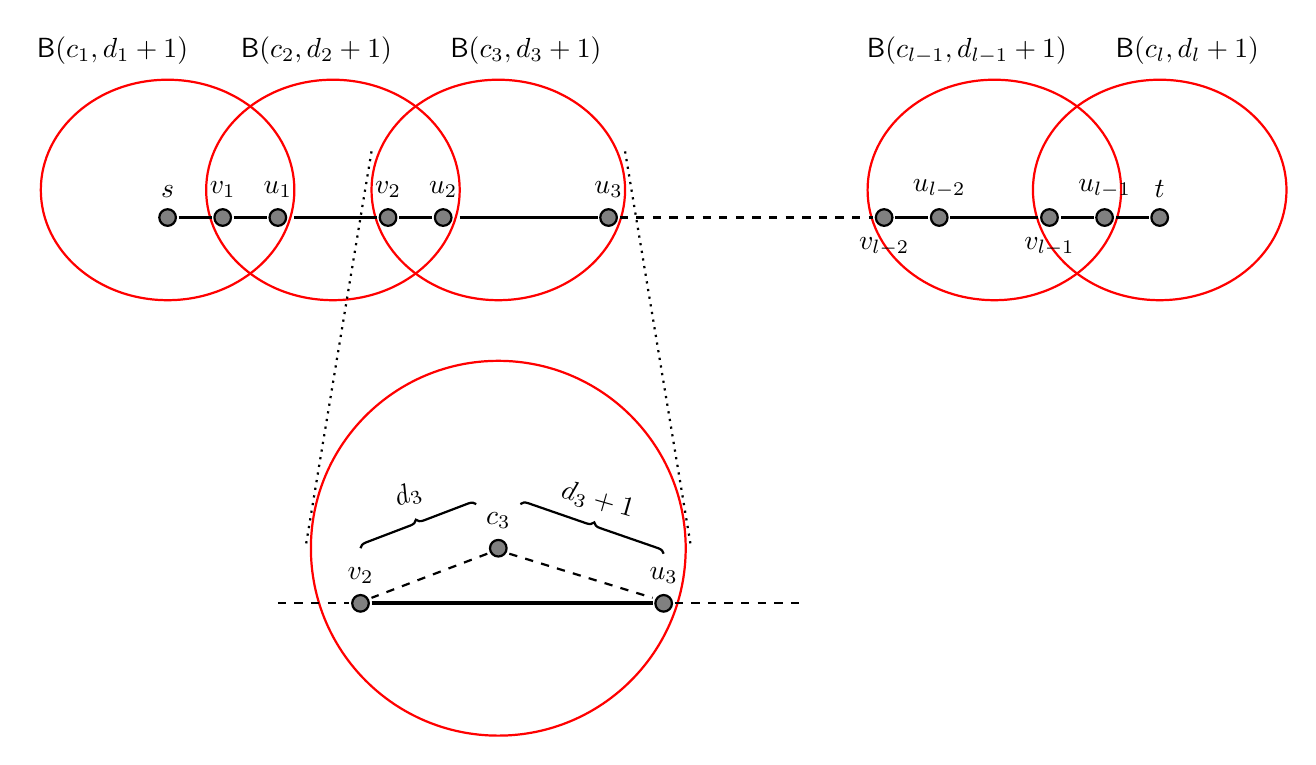
\begin{tikzpicture}[thick,scale=0.7]
	\draw [red] (15, 0.5) ellipse (2.3 and 2);
	\draw [red] (0, 0.5) ellipse (2.3 and 2);
	\draw [red] (3, 0.5) ellipse (2.3 and 2);
	\draw [red] (6, 0.5) ellipse (2.3 and 2);
	\draw [red] (18, 0.5) ellipse (2.3 and 2);
	
	\draw (0, 0) node[circle, draw, fill=black!50, inner sep=0pt, minimum width=6pt, label = $s$] {};
	\draw (18, 0) node[circle, draw, fill=black!50, inner sep=0pt, minimum width=6pt,label = $t$] {};
	
	\draw (2, 0) node[circle, draw, fill=black!50, inner sep=0pt, minimum width=6pt,label = $u_1$] {};
	\draw (1, 0) node[circle, draw, fill=black!50, inner sep=0pt, minimum width=6pt,label = $v_1$] {};
	\draw [line width = 0.5mm] (0.2, 0) -- (0.8, 0);
	\draw [line width = 0.5mm] (1.2, 0) -- (1.8, 0);
	
	\draw (-1, 2.4) node[red, label={$\ball(c_1, d_{1}+1)$}]{};
	
	\draw (5, 0) node[circle, draw, fill=black!50, inner sep=0pt, minimum width=6pt,label = $u_2$] {};
	\draw [line width = 0.5mm] (2.3, 0) -- (3.8, 0);
	\draw [line width = 0.5mm] (4.2, 0) -- (4.8, 0);
	
	\draw (2.7, 2.4) node[red, label={$\ball(c_2, d_{2}+1)$}]{};
	
	\draw (4, 0) node[circle, draw, fill=black!50, inner sep=0pt, minimum width=6pt,label = $v_2$] {};
	\draw (8, 0) node[circle, draw, fill=black!50, inner sep=0pt, minimum width=6pt,label = $u_3$] {};
	\draw [line width = 0.5mm] (5.3, 0) -- (7.8, 0);
	
	\draw (6.5, 2.4) node[red, label={$\ball(c_3, d_{3}+1)$}]{};
	
	\draw[dotted] (3.7, 1.2) -- (2.5, -6);
	\draw[dotted] (8.3, 1.2) -- (9.5, -6);
	\draw (3.5, -7) node[circle, draw, fill=black!50, inner sep=0pt, minimum width=6pt,label = $v_2$] {};
	\draw (9, -7) node[circle, draw, fill=black!50, inner sep=0pt, minimum width=6pt,label = $u_3$] {};
	\draw (6, -6) node[circle, draw, fill=black!50, inner sep=0pt, minimum width=6pt,label = $c_3$] {};
	\draw [red] (6, -6) ellipse (3.4 and 3.4);
	\draw [line width = 0.5mm] (3.7, -7) -- (8.8, -7);
	\draw [dashed] (2, -7) -- (3.3, -7);
	\draw [dashed] (9.2, -7) -- (11.5, -7);
		\draw [decorate,
	decoration = {brace}] (3.5,-6) -- (5.6,-5.2);
	\draw (4.5, -5.6) node[label={[rotate=20]$d_3$}]{};
	\draw [dashed] (5.8, -6.1) -- (3.7, -6.9);
	\draw [decorate,
	decoration = {brace}] (6.4,-5.2) -- (9,-6.1);
	\draw (7.7, -5.7) node[label={[rotate=-16]$d_3+1$}]{};
	\draw [dashed] (6.2, -6.1) -- (8.8, -6.9);
	
	\draw (16, 0) node[circle, draw, fill=black!50, inner sep=0pt, minimum width=6pt,label = -90: $v_{l-1}$] {};
	\draw (17, 0) node[circle, draw, fill=black!50, inner sep=0pt, minimum width=6pt,label = $u_{l-1}$] {};
	\draw [line width = 0.5mm] (17.8, 0) -- (17.2, 0);
	\draw [line width = 0.5mm] (16.8, 0) -- (16.2, 0);

	
	\draw (18.5, 2.4) node[red, label={$\ball(c_l, d_{l}+1)$}]{};
	
	\draw (13, 0) node[circle, draw, fill=black!50, inner sep=0pt, minimum width=6pt,label = -90 : $v_{l-2}$] {};
	\draw (14, 0) node[circle, draw, fill=black!50, inner sep=0pt, minimum width=6pt,label = $u_{l-2}$] {};
	\draw [line width = 0.5mm] (13.8, 0) -- (13.2, 0);
	\draw [line width = 0.5mm] (15.8, 0) -- (14.2, 0);
	
	\draw (14.5, 2.4) node[red, label={$\ball(c_{l-1}, d_{{l-1}}+1)$}]{};
	
	\draw [dashed] (8.2, 0) -- (12.8, 0);
\end{tikzpicture}
	\end{center}
	\caption{The construction of sequences $u_1, u_2, \ldots, u_l$ and $v_1, v_2, \ldots, v_{l-1}$.}\label{terminal}
\end{figure}
%
%Pick the shortest path $\pi$ from $s$ to $t$ under the random perturbations. During the iterations, we will maintain two sequences of vertices $u_0 = s, u_1, u_2, \cdots, u_l$, $v_0 = s, v_1, v_2, \cdots, v_{l-1}$, a sequence of paths $\beta_1, \beta_2, \cdots, \beta_l$, and a sequence of small balls $\ball(c_1, r_{1}), \ball(c_2, r_{2}), \cdots, \ball(c_l, r_{l})\in \clusters$, with the following properties.
\iffalse
\begin{enumerate}[(i)]
\item %$u_1, u_2, \cdots, u_l$, $v_1, v_2, \cdots, v_{l-1}$ are vertices on $\pi$ following the direction from $s$ to $t$, 
for each $1\leq i\leq l-1$, $v_i$ on the sub-path $\pi[u_{i-1}, u_i], \forall 1\leq i\leq l-1$.
\item $v_0\in \ball(c_1, d_{1})$, and $v_i\in \ball^=(c_{i+1}, d_{{i+1}}), u_i\in \ball^=(c_i, d_{i}+1), \forall 1\leq i\leq l-1$. Also, if $u_l\neq t$, $u_l\in \ball^=(c_l, d_{l}+1)$.
\end{enumerate}
\fi

This is done via an iterative process described as the following steps. 

\begin{enumerate}[(1),leftmargin=*]
	\item Start with $i=0$ and set $u_0=v_0=s$. If $u_i = t$ then we terminate the process and set $l=i+1$.
	
	Otherwise, we find the ball in $\clusters_1$ that, among all balls in $\clusters_1$ that intersects $\pi[s, u_i]$, the one that contains a vertex on $\pi$ that is \textbf{closest} to $t$. In other words, if we denote $\pi$ as $(s=w_0,w_1,\ldots,w_{k-1},w_k=t)$, then we find the ball that intersects $\pi[s, u_i]$, and, subject to this, contains a vertex $w_j$ with the largest index.
	
	Note that such a ball always exists; for example, we can take an arbitrary ball in $\bset_1$ that contains $u_i$, and we can also notice that $u_{i+1}$ should belong to $\pi(u_i, t]$.
	
	We denote this ball by $\ball(c_{i+1}, d_{i+1})$ and set $u_{i+1}$ as the last vertex of $\pi$ that belongs to  $\ball(c_{i+1}, d_{i+1}+1)$. 
	
	\item If $i\ge 1$, we then let $v_i$ be any vertex that belongs to both $\pi[u_{i-1}, u_i]$ and $\ball^=(c_{i+1}, d_{i+1})$. We will prove shortly that such $v_i$ always exists.
	
	Then, increase $i\leftarrow i+1$ and go to Step (1).
\end{enumerate}

We now turn to argue the existence of $v_i$.

\begin{claim}
For each $i\ge 1$, $\pi[u_{i-1}, u_i]$ intersects with $\ball^=(c_{i+1}, d_{i+1})$, and if $u_{i+1}\neq t$, then $u_{i+1}\in \ball^=(c_{i+1}, d_{i+1}+1)$.
\end{claim}
\begin{proof}[Proof of claim]
First, if $\pi[s, u_i]$ does not intersect $\ball^=(c_{i+1}, d_{i+1})$, as $\pi[s, u_i]$ intersects $\ball(c_{i+1}, d_{i+1})$, it has to lie entirely within $\ball(c_{i+1}, d_{i+1})$, a contradiction to the choice of $\ball(c_1, d_{1})$ and $u_1$. Therefore, $\pi[s, u_i]$ intersect $\ball^=(c_{i+1}, d_{i+1})$. 

We now claim any such intersection $v_i$ must belong to $\pi[u_{i-1}, u_i]$. Otherwise, if $v_i$ belongs to $\pi[u_{j-1}, u_j]$ for some index $1\leq j<i$, then earlier when we were determining $u_{j+1}$, it should have been at least as close to $t$ as $u_{i+1}$, a contradiction to the property that $u_i\in (u_j,t]$.
%\tnote{According to this new definition, it is not guaranteed that $u_i\in (u_j, t]$.}
%

Lastly, if $u_{i+1}\in \ball(c_{i+1}, d_{i+1})$, then the next vertex on path $\pi$ should also belong to $\ball(c_{i+1}, d_{i+1}+1)$, a contradiction to the choice of $u_{i+1}$.
\end{proof}
		
%Finally, assign $\ball(c_{l+1}, d_{{l+1}})\leftarrow \ball(c, r)$, and increment $l\leftarrow l+1$ and go to Step (2).
%\end{enumerate}
	
It is clear that when the iterative process terminates, $u_l = t$. We now show that for each $2\leq i\leq l-1$, the subpath $\pi[v_{i-1}, u_i]$ is contained in $H$. Note that $v_{i-1}\in \ball^=(c_i, d_{i})$ and $u_i\in \ball^=(c_i, d_{i}+1)$. Since $\ball(c_i, r_{i})$ is small, from the algorithm, we have constructed a subgraph $L_c$ in $G[\ball(c_i, 4r_{i})]$ that preserves all-pairs distances between vertices in $\ball^=(c_i, d_{i})\cup \ball^=(c_i, d_{i}+1)$. As the shortest path between every pair of vertices is unique, the subpath $\pi[v_{i-1}, u_i]$ should be entirely contained in $L_c$.
%\tnote{Shortest paths in unweighted graphs are not unique.}
%by directly adding the shortest paths under random perturbations. Since $\pi$ is the shortest path from $s$ to $t$ under the random perturbations, its sub-path $\pi[v_{i-1}, u_i]$ should belong to the distance preserver which is in spanner $H$. See Figure \ref{terminal} for an illustration.
	
	
Lastly, we consider the distance in $H$ between the endpoints $s, t$ of $\pi$. From the construction, we know that vertices $s, u_1\in \ball(c_1, d_{1}+1)$, and $v_{l-1}, t\in \ball(c_l, d_{l}+1)$. Therefore, $\dist_H(s, u_1) \le  4Rn^\epsilon$, and $\dist_H(v_{l-1}, t) \le 4Rn^\epsilon$. It follows that $\dist_H(s, t)\leq \dist_{G}(s, t) + 8Rn^\epsilon$. Furthermore, if both $s, t$ are covered at boundary by $\clusters_1$, then $s\in \ball^=(c_1, d_{1})$ and $t\in \ball^=(c_l, d_{l})$. Therefore, the entire path $\pi$ belongs to $H$, and so $\dist_H(s, t) = \dist_{G}(s, t)$.
\end{proof}

We now focus on the algorithm for handling large balls.  Consider an iteration in which a shortest path $\pi_{s, t}$ is processed for some pair $s, t\in U$. We prove the following claims.

\begin{claim}\label{boundary}
Let $\pi_{s, t}[u, v]$ be a maximal subpath of $\pi_{s, t}$ consisting of only vertices covered by $\bset_1$. If $u\ne s$ and $v\ne t$, then both $u, v$ are covered at boundary by $\bset_1$.
\end{claim}
\begin{proof}
Assume for contradiction that $u$ belongs to a ball $\ball(c, d-1)$ for some small ball $\ball(c, r)\in\clusters$. Let $(w, u)$ be the last edge of subpath $\pi_{s, t}[s, u]$, then $w\in\ball(c, d)$, and so $w$ is also covered. Therefore, $\pi_{s, t}[w, v]$ should be a covered subpath, which contradicts the maximality of subpath $\pi_{s, t}[u, v]$.
\end{proof}

\begin{claim}\label{Uc}
For any large ball $\ball(c, r)$ and every vertex $s\in U_c$, $\dist_H(s, c)\leq \dist_{G}(s, c) + 10Rn^\epsilon$.
\end{claim}
\begin{proof}
Let $\pi_{s, t}$ be the shortest path that was processed in the iteration where $s$ was added to $U_c$. 
%From the algorithm, we can see that the union of paths in all $\Delta\paths_c$ is equal to the union of all uncovered sub-paths of $\pi_{s, t}$. Therefore, after Step (5), all uncovered sub-paths of $\pi_{s, t}$ are added to spanner $H$. Take an arbitrary sub-path $\pi_{s, t}[u, \cdot]\in \Delta\paths_c$. 
By the algorithm, $\ball(c, r)$ must be referring to some ball $\ball(c_x, r_x)$ for some $x\in \pi_{s, t}$. As $H$ contains a BFS tree that is rooted at $c$ and contains $x$, and the radius of each ball is at most $2Rn^{\eps}$, it suffices to show that $\dist_H(s, x)\leq \dist_{G}(s, x) + 8Rn^\epsilon$.

%Consider all the Type (A) and Type (B) sub-paths on $\pi_{s, t}[s, u]$. Since all Type (B) sub-path edges are now in $H$, we only need to focus on the additive error contributed by Type (A) sub-paths. 
Recall that path $\pi_{s, t}$ was partitioned into subpaths in sets $\Sigma$ and $\Sigma^\prime$. From the algorithm description, all subpaths in $\Sigma'$ are entirely contained in $H$.
For every subpath $\pi_{s, t}[y, z]$ of $\pi_{s, t}$ in $\Sigma$, if $y\neq s$, then from \Cref{exact} and \Cref{boundary}, $\dist_H(y, z) = \dist_{G}(y, z)$; if $y = s$, then from \Cref{exact}, we get that $\dist_H(y, z) \leq \dist_{G}(y, z) + 8Rn^\epsilon$. Since there is at most one subpath $\pi_{s, t}[y, z]$ in $\Sigma$ with $y = s$, the overall additive error caused by subpaths in $\Sigma$ is at most $8Rn^\epsilon$.
\end{proof}

\begin{claim}[additive error]
For every pair  $s, t\in U$, $\dist_H(s, t)\leq \dist_{G}(s, t) + 24Rn^\epsilon$.
\end{claim}
\begin{proof}
Consider the iteration when $\pi_{s, t}$ was processed.
If $\pi_{s, t}$ is entirely covered by $\clusters_1$, %(namely, $\pi_{s, t}$ itself is of Type (A)), 
then the claim follows from \Cref{exact}. 
If not, then from the algorithm, after this iteration some large ball $\ball(c, r)\in\clusters$ intersecting $\pi_{s, t}$ must have added $s, t$ into its set $U_c$. Then from \Cref{Uc}, 
$$\dist_{H}(s, c)\leq \dist_{G}(s, c) + 10Rn^\epsilon,$$
$$\dist_H(c, t)\leq \dist_{G}(c, t) + 10Rn^\epsilon.$$
Let $v$ be an arbitrary vertex in $\ball(c, r)\cap V(\pi_{s, t})$. By triangle inequality,
\[\dist_{G}(s, c) + \dist_{G}(c, t) \leq \dist_G(s, v) + \dist_G(v, t) + 2\cdot \dist(v, c) \leq \dist_G(s, t) + 4Rn^\epsilon.\]
Altogether, $\dist_H(s, t)\leq \dist_{G}(s, t) + 24Rn^\epsilon$.
\end{proof}


\subsection{Size and runtime analysis}

\begin{claim}[spanner size]
$|E(H)|=O\brac{2^{O(1/\epsilon)}\cdot n\log n}$.
\end{claim}
\begin{proof}
\iffalse
From the algorithm, for each large ball $\ball(c,r)\in \bset$, every time a new path is added to $\Pi_c$, the size of $|U_c|$ also increases by at least one, so eventually $|\paths_c|\le |U_c|\le |U|$. As the shortest paths after edge pertubation are unique (and therefore consistent), from \Cref{consist}, 
$$|E(\Pi_c)|\le O(|\ball(c, 4r)| + \sqrt{|\ball(c, 4r)|}\cdot |\paths_c|) \leq O(|\ball(c, 4r)| + \sqrt{|\ball(c, 4r)|}\cdot |U|)\leq O(2^{5/\epsilon}|\ball(c, 4r)|)$$
Summing over all large balls,  $\sum_c|E(\Pi_c)| =\sum_{c}O(2^{5/\epsilon}|\ball(c, 4r)|) = O(2^{15/\epsilon}n/\eps)$. Combined with previous bounds on the number of edges in small balls and in BFS trees, $|E(H)|=2^{O(1/\epsilon)}\cdot n$.
\fi
It suffices to bound the total number of edges added to $H$ when handling large balls. For each large ball $\ball(c, r)\in \bset$, let us conceptually construct a set $\Pi_c$ of paths within $G[\ball(c, 4r)]$ during handling large balls.

Initially, all sets $\Pi_c$ are empty. When processing a path $\pi_{s, t}\in \Pi$, suppose Step (3) is executed. Consider the set of large balls $\{\ball(c_x, r_x)\mid x\in \pi_{s, t} \}$. For any ball $\ball(c, r)\in \{\ball(c_x, r_x)\mid x\in \pi_{s, t} \}$, let $y, z\in \ball(c, r+1)\cap \pi_{s, t}$ be the first and the last vertex on $\pi_{s, t}$. Then, add the subpath $\pi_{s, t}[y, z]$ to $\Pi_c$. Note that this path $\pi_{s,t}$ lies entirely in $G[\ball(c, 4r)]$.

We first show that in the end, all edges added to $H$ for handling large balls is a subset of $E\left(\bigcup_{\ball(c, r)\in \bset\text{ is large}} \Pi_c\right)$. When processing a path $\pi_{s, t}\in \Pi$, consider any vertex $x$ on a sub-path $\rho\in\Sigma^\prime$ which is not an endpoint of $\rho$. Then, since $x$ is not covered by $\bset_1$, any ball that covers $x$ must be large, and in particular $\ball(c_x, r_x)$ should be large. Suppose $y, z\in \ball(c_x, r_x+1)$ are the first and the last vertex on $\pi_{s, t}$. Then, $\pi_{s, t}[y, z]$ must contain all edges incident on $x$ on $\rho$. Hence, the union of all $\pi_{s, t}[y, z]$ ranging over all $x$'s should contain all paths in $\Sigma^\prime$.

Next, we show that $|\Pi_c|\leq |U|$ for any $c$. In fact, each time we added a new path to $\Pi_c$, we must have added $s, t$ to $U_c$ which increased $|U_c|$. Since $U_c\subseteq U$, we know that $|\Pi_c|\leq |U|$ in the end.

Finally, it suffices to bound the number of edges in $E\left(\bigcup_{\ball(c, r)\in \bset\text{ is large}} \Pi_c\right)$. Using \Cref{consist}, we have: 
$$E(\Pi_c)\leq O\left(|\ball(c, 4r)| + \sqrt{\ball(c, 4r)}\cdot |\Pi_c|\right)\leq O\left(|\ball(c, 4r)|\right).$$
Hence, $$E\left(\bigcup_{\ball(c, r)\in \bset\text{ is large}} \Pi_c\right)\leq O\left(\sum_{\ball(c, r)\in \bset\text{ is large}}|\ball(c, 4r)|\right) = O\brac{2^{O(1/\epsilon)}\cdot n\log n}.$$
\end{proof}

\begin{claim}[runtime]
The runtime of the algorithm is $O\big(m\big(|U| + 2^{O(1/\epsilon)}\big)\big)$.
\end{claim}
\begin{proof}
From \Cref{clustering}, computing all the balls in $\clusters$ takes time at most $O(2^{10/\epsilon}m/\eps)$. From \Cref{cor: BFS consistent}, constructing graphs $L_c$ in all small balls takes time at most $O(|U|^{1/2}\sum_c \vol_{G}(\ball(c, 4r)))=O(|U|^{1/2}m \cdot 2^{10/\eps}/\eps)$, and computing the paths in $\Pi$ takes time $O(m|U|)$. As for the part with large balls, the runtime is dominated by scanning all shortest paths $\pi_{s, t}$ in $\Pi$, which takes time at most $O(n|U|)$. Overall, the runtime is $O\big(m\big(|U| + 2^{O(1/\epsilon)}\big)\big)$.
\end{proof}

\section{Linear-Size Additive Spanners in Sub-quadratic Time}
\label{sec: subq}

In this section we provide the proof of \Cref{subquad}. 
We will first show in \Cref{sec: subquad for 3/7} a simple subquadratic time algorithm for computing an $\tilde O(n^{3/7+\eps})$ additive spanner.
Then we will slightly modify it to achieve better additive error bound in \Cref{sec: proof of subquad}.

\subsection{A subquadratic time algorithm for $\tilde O(n^{3/7+\eps})$ additive spanner}
\label{sec: subquad for 3/7}

In this subsection, we prove the following theorem, which shows that an additive spanner with the current best error (as in \cite{bodwin2021better}) can be computed in subquadratic time.

\begin{theorem}\label{subquad for 3/7}
There is an algorithm, that, given any undirected unweighted graph on $n$ vertices and $m$ edges, and any parameter $\eps > 0$, computes a spanner on $O\brac{2^{O(1/\eps)}\cdot n\log n}$ edges with $\tilde O(n^{3/7+\eps})$ additive stretch, in time $\tilde{O}\big(m + 2^{O(1/\eps)}\cdot n^{13/7}\big)$.
\end{theorem}
\begin{remark}
	If we do not care about the runtime constraint, then the spanner size can be made $2^{O(1/\epsilon)}n$ by replacing \Cref{clustering} with the original Lemma 13 from \cite{bodwin2021better}.
\end{remark}

We start with the following lemma for a preliminary sparsification of the input graph.
%Since we are aiming for $\tilde{O}(n^{3/7+\epsilon})$ additive stretch, the following lemma says that we can safely assume $G$ is a sparse graph.
\begin{lemma}\label{preproc}
There is an algorithm, that given any graph $G$ and parameter $1<d<n$, computes in $\tilde{O}(m)$ time an $+\tilde O(n/d)$ spanner $G'$ of $G$ with $|E(G')|\le O(nd)$ edges.
%such that for any $s, t\in V$, we have $\dist_{G^\prime}(s, t)\leq \dist_G(s, t) + \tilde{O}(n/d)$; plus, $G^\prime$ can be constructed 
\end{lemma}
\begin{proof}
Graph $G^\prime$ is simply the union of (i) for each vertex $v\in V(G)$ with $\deg_G(v) \leq \ceil{d}$, all incident edges of $v$; and (ii) an $O(\log n)$-multiplicative spanner of $G$ with $O(n)$ edges; such a multiplicative spanner can be computed in $\tilde{O}(m)$ time as shown in \cite{baswana2007simple}. Clearly, graph $G'$ can be computed in $\tilde O(m)$ time.
	
Consider now any pair $s, t\in V(G)$ and let $\pi$ be an $s$-$t$ shortest path in $G$. 
It is easy to observe that at most $O(n/d)$ vertices in $\pi$ have degree more than $d$, so the number of edges in $E(\pi)$ that is incident to any degree $\le d$ vertex is at most $O(n/d)$. As we have included in $G'$ an $O(\log n)$-multiplicative spanner of $G$, the distance in $G'$ between the pair of endpoints of every such edge is at most $O(\log n)$.
Therefore, $\dist_{G'}(s,t)\le \dist_G(s,t)+\tilde{O}(n/d)$.
\end{proof}

We now proceed to describe our algorithm for \Cref{lem: reduction}. Similar to \Cref{sec: subset}, we assume that the (unit) edge weights are slightly perturbed so that for every pair $s,t$ there is a unique shortest path connecting them in $G$ (or any subgraph that contains both $s$ and $t$).

As a pre-processing step, if $|E(G)|\ge 10\cdot n^{2-3/7}$, then we first apply the algorithm from \Cref{preproc} to $G$ with $d=n^{1-3/7}$,
%By the above lemma, choosing $d = \ceil{n^{3/7}}$, for the rest we reduce to the case where $G$ itself has at most $O(n^{11/7})$ edges by a $\tilde{O}(m)$ runtime overhead.
and get graph $G'$, so $|E(G')|=O(n^{2-3/7})$.
If $|E(G)|\le 10\cdot n^{2-3/7}$, then we simply set $G'=G$.

%Without loss of generality, Note that we can assume that $G$ is connected, as otherwise we simply focus on different connected components of $G$, so $$.  
%The main algorithm utilizes the power of Lemma \ref{clustering}. 
We then apply the algorithm from \Cref{clustering} to $G'$ with parameter $R$ (to be determined later) and $\frac{10}{\epsilon\log_2n}$, and let $\bset$ be the set of balls we obtain.
%
\iffalse
each radius $r = [R, Rn^\epsilon]$ in $\tilde{O}(2^{10/\epsilon}m)$ time with two properties:
 \begin{itemize}
	\item (Coverage) For each $v\in V$, there is some ball such that $v\in \ball_G(c, r)\in \bset$.
	\item (Disjointness) $\sum_{\ball(c, r)\in\bset}|\ball(c, 4r)| = \tilde{O}(2^{10/\epsilon}n)$, $\sum_{\ball(c, r)\in\bset}\vol(\ball(c, 4r)) = \tilde{O}(2^{10/\epsilon}m)$.
\end{itemize}

For any ball $\ball(c, r)\in\bset$, classify it as one of the following two types.
\begin{itemize}
	\item (Small) $|\ball(c, r)| \leq R^{5/3}$.
	\item (Large) $|\ball(c, r)| > R^{5/3}$.
\end{itemize}
\fi 
We say that a ball $\ball(c, r)\in\bset$ is \emph{small} if $|\ball(c, r)| \leq R^{5/3}$; otherwise we say it is \emph{large}.
For each ball $\ball(c,r)\in \balls$, we compute a BFS tree $T_c$ that is rooted at $c$ and spans all vertices in $\ball(c, 4r)$, in time $O(\vol(\ball(c, 4r)))$. From \Cref{clustering}, $\sum_{c} |E(T_c)|= \sum_{c} |\ball(c, 4r)| = O(2^{10/\epsilon}n\log n)$.



%For the rest we will mainly work on the sparse graph $G$. Let $H$ denote the target additive spanner of $G$. $H$ is constructed from an empty graph. First, for each ball $\ball(c, r)\in \bset$, add an arbitrary breath-first search tree at $c$ that spans $\ball(c, 4r)$ to $H$. Next, add two different types of subset spanners to $H$.
%\vspace{-10pt}

\paragraph{Handling small balls.} Consider a small ball $\ball(c, r)\in \bset$. From Lemma \ref{bottleneck}, we can compute in time $O(\vol(\ball(c, 4r)))$ an integer $d\in [r, 2r]$ such that $|\ball^=(c, d)\cup\ball^=(c, d+1)|\leq 2|\ball(c, 4r)| / r \leq 2|\ball(c, 4r)| / R$. We denote  %For notational convenience, denote: 
$\bset_1 = \{\ball(c, d)\mid \ball(c, r)\in\bset\text{ is small} \}$.
%Next, we will build a distance preserver $X_c\subseteq G[\ball(c, 4r)]$ such that $\dist_{X_c}(s, t) = \dist_{G}(s, t)$ for any pair $s, t\in \ball^=(c, d)\cup\ball^=(c, d+1)$. To do this, go over each vertex $s\in \ball^=(c, d)$ and compute single-source shortest paths at $s$ in $G[\ball(c, 4r)]$. By doing so, we can collect a set $\Pi_c = \{\pi_{s, t} \mid s, t\in \ball(c, d)\cup\ball(c, d+1) \}$ of shortest paths between any pair of vertices in $\ball(c, d)\cup\ball(c, d+1)$; we can make sure that $\paths$ is consistent by randomly perturbing the unit edge weights of $G[\ball(c, 4r)]$. 
%We then apply the algorithm from \Cref{cor: BFS consistent} to the induced subgraph $G[\ball(c, 4r)]$ with $S=T=\ball^=(c, d)\cup\ball^=(c, d+1)$, and obtain a collection $\Pi_c$ of shortest paths. We define $R_c=\bigcup_{\pi\in \Pi_c}\pi$.
%Add all edges in $\bigcup_{c, \pi\in \Pi_c}\pi$ to $X$. According to Lemma \ref{consist}, each path system $\Pi_c$ contains edges at most 
%From \Cref{cor: BFS consistent} and \Cref{clustering}, $$\sum_{c} |E(R_c)|= \sum_{c} O\left(|\ball(c, 4r)| + \sqrt{|\ball(c, 4r)|}\cdot \left(\frac{|\ball(c, 4r)|}{R}\right)^2\right) = \sum_c O(2^{15/\epsilon}|\ball(c, 4r)|)=O(2^{25/\epsilon}n/\eps)$$
\iffalse
\paragraph{Local subset spanner.} For each small ball $\ball(c, r)\in \bset$, apply Lemma \ref{bottleneck} to find a radius $d\in [r, 2r]$ such that $|\ball^=(c, d)\cup\ball^=(c, d+1)|\leq 2|\ball(c, 4r)| / r$; also when $\ball(c, r)$ is large, simply set $d = r$. For notational convenience, define 
$$\bset_1= \{\ball(c, d)\mid \ball(c, r)\in\bset\}$$
\fi
Then, for each small ball $\ball(c, r)$, apply Lemma \ref{subset} to compute a subset spanner $L_c$ of $G'[\ball(c, 4r)]$ on the set $\ball^=(c, d)\cup\ball^=(c, d+1)$.

%\paragraph{Global subset spanner.} Sample a random vertex subset $S$ of size $\ceil{10R^{2/3}\log n}$ from the multi-set $$\biguplus_{\ball(c, r)\in \bset}\ball(c, 4r)$$ 

%\vspace{-10pt}

\paragraph{Handling large balls.}
Choose a random subset $S\subseteq V(G)$ of size $\ceil{10R^{2/3}\log n}$.
% from the multi-set $\biguplus_{\ball(c, r)\in \bset}\ball(c, 4r)$.
We then apply Lemma \ref{subset} to compute a subset spanner $\hat H$ of $G'$ on $S$.

\paragraph{The spanner construction.}
The output graph $H$ is simply defined to be the union of 
\begin{itemize}
	\item for each ball $\ball(c,r)\in \balls$, the tree $T_c$;
	\item for each small ball $\ball(c,r)\in \balls$, graph $L_c$;
	\item graph $\hat H$.
\end{itemize}


\subsubsection{Stretch analysis}

According to \Cref{preproc}, in order to show that $H$ is a $+\tilde O(n^{3/7+\eps})$ spanner of $G$, it suffices to show that $H$ is a $+\tilde O(n^{3/7+\eps})$ spanner of $G'$. For notational convenience, in this subsection we rename $G'$ by $G$.
%
The following statement, which is a generalization of \Cref{exact}, is the key to the stretch analysis.
\begin{claim}\label{exact2}
Let $s,t$ be a pair of vertices in $G$ and let $\pi$ be a shortest path connecting them. Then there exists (i) a path $\phi$ in $H$ connecting $s$ to $t$; (ii) a sequence of balls $\ball(c_1, r_{1}), \ldots, \ball(c_l, r_{l})$; (iii) two sequences of vertices $(u_0 = s, u_1, \ldots, u_l = t)$ and $(v_0 = s, v_1, \ldots, v_{l-1})$, and two sequences of paths  $\alpha_1, \alpha_2, \ldots, \alpha_l$, $\beta_1, \beta_2, \ldots, \beta_l$, with the following properties.
	\begin{enumerate}[(a),leftmargin=*]
		\item Vertices $u_1, u_2, \ldots, u_l$ appear on path $\pi$ in this order in the direction from $s$ to $t$.
		\item $s\in \ball(c_1, d_{1}), t\in\ball(c_l, d_{l}+1)$, and $v_i\in \ball^=(c_{i+1}, d_{{i+1}}), u_i\in \ball^=(c_i, d_{i}+1), \forall 1\leq i\leq l-1$.
		\item For each $1\leq i\leq l$, $\alpha_i$ is a shortest path in $H$ connecting $v_{i-1}$ to $u_i$ that is entirely contained in $G[\ball(c_i, 4r_{i})]$, and moreover, vertex $v_i$ lies on $\alpha_i$.
		\item For each $1\leq i\leq l-1$, $\beta_i = \alpha_i[v_{i-1}, v_i]$; and $\beta_l = \alpha_l$.
		\item $\phi=\beta_1\circ \cdots \circ \beta_l$; and $|\phi|\leq \dist_{G}(s, t) + 15\cdot Rn^\epsilon + \tilde{O}\left(2^{15/\epsilon}\cdot n^\epsilon\cdot\sum_{i=2}^{l-1}\frac{|\ball(c_i, r_{i})|}{R^{2/3}}\right)$.
	\end{enumerate}
\end{claim}

\begin{figure}[h]
	\begin{center}
		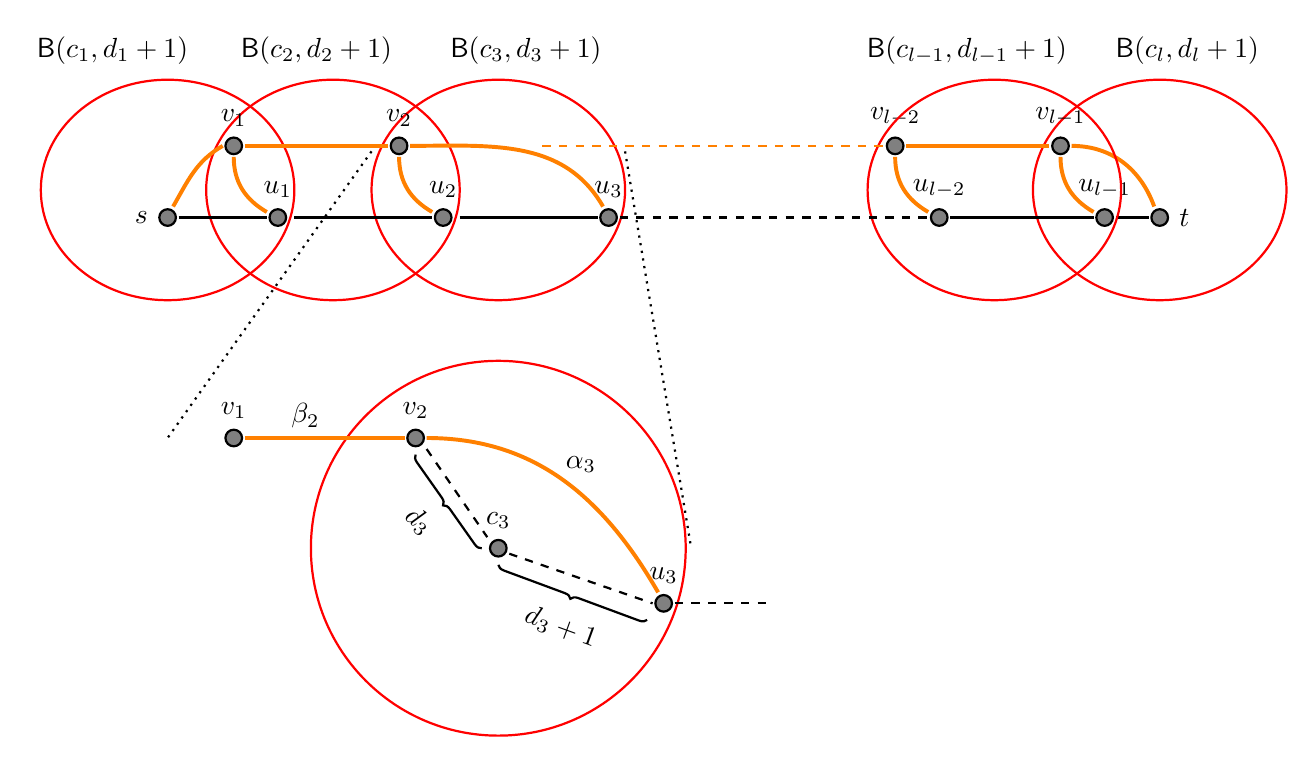
\begin{tikzpicture}[thick,scale=0.7]
	\draw [red] (0, 0.5) ellipse (2.3 and 2);
	\draw [red] (3, 0.5) ellipse (2.3 and 2);
	\draw [red] (6, 0.5) ellipse (2.3 and 2);
	\draw [red] (18, 0.5) ellipse (2.3 and 2);
	
	\draw (0, 0) node[circle, draw, fill=black!50, inner sep=0pt, minimum width=6pt, label = 180 : $s$] {};
	\draw (18, 0) node[circle, draw, fill=black!50, inner sep=0pt, minimum width=6pt,label = 0 : $t$] {};
	
	\draw (2, 0) node[circle, draw, fill=black!50, inner sep=0pt, minimum width=6pt,label = $u_1$] {};
	\draw (1.2, 1.3) node[circle, draw, fill=black!50, inner sep=0pt, minimum width=6pt,label = $v_1$] {};
	\draw [line width = 0.5mm] (0.2, 0) -- (1.8, 0);
	\draw [line width = 0.5mm, color=orange] (0.1, 0.2) to[out=60, in=210] (1, 1.3);
	\draw [line width = 0.5mm, color=orange] (1.2, 1.1) to[out=-90, in=150] (1.8, 0.1);
	
	\draw (-1, 2.4) node[red, label={$\ball(c_1, d_{1}+1)$}]{};
	
	\draw (5, 0) node[circle, draw, fill=black!50, inner sep=0pt, minimum width=6pt,label = $u_2$] {};
	\draw [line width = 0.5mm] (2.3, 0) -- (4.8, 0);
	
	\draw (2.7, 2.4) node[red, label={$\ball(c_2, d_{2}+1)$}]{};
	\draw [line width = 0.5mm, color=orange] (1.4, 1.3) -- (4, 1.3);
	\draw [line width = 0.5mm, color=orange] (4.2, 1.1) to[out=-90, in=150] (4.8, 0.1);
	
	\draw (4.2, 1.3) node[circle, draw, fill=black!50, inner sep=0pt, minimum width=6pt,label = $v_2$] {};
	\draw (8, 0) node[circle, draw, fill=black!50, inner sep=0pt, minimum width=6pt,label = $u_3$] {};
	\draw [line width = 0.5mm] (5.3, 0) -- (7.8, 0);
	
	\draw (6.5, 2.4) node[red, label={$\ball(c_3, d_{3}+1)$}]{};
	\draw [line width = 0.5mm, color=orange] (4.4, 1.3) to[out=0, in=120] (7.9, 0.2);
	
	\draw[dotted] (3.7, 1.2) -- (0, -4);
	\draw[dotted] (8.3, 1.2) -- (9.5, -6);
	\draw (4.5, -4) node[circle, draw, fill=black!50, inner sep=0pt, minimum width=6pt,label = $v_2$] {};
	\draw (9, -7) node[circle, draw, fill=black!50, inner sep=0pt, minimum width=6pt,label = $u_3$] {};
	\draw (6, -6) node[circle, draw, fill=black!50, inner sep=0pt, minimum width=6pt,label = $c_3$] {};
	\draw [red] (6, -6) ellipse (3.4 and 3.4);
	%\draw [dashed] (2, -7) -- (8.8, -7);	
	\draw [dashed] (9.2, -7) -- (11, -7);
	\draw [line width = 0.5mm, color=orange] (4.7, -4) to[out=0, in=120] (8.9, -6.8);
	\draw (7.5, -5) node[red, label={$\alpha_3$}]{};
	\draw [line width = 0.5mm, color=orange] (1.4, -4) to (4.3, -4);
	\draw (1.2, -4) node[circle, draw, fill=black!50, inner sep=0pt, minimum width=6pt,label = $v_1$] {};
	\draw (2.5, -4.2) node[red, label={$\beta_2$}]{};
	
	\draw [decorate, decoration = {brace}] (5.7,-6) -- (4.5,-4.3);
	\draw [dashed] (4.7, -4.2) -- (5.8, -5.8);
	\draw (4.3, -6) node[label={[rotate=-40]$d_3$}]{};
	\draw [decorate, decoration = {brace}] (8.7, -7.3) -- (6, -6.3);
	\draw [dashed] (6.2, -6.1) -- (8.8, -7);
	\draw (7, -8) node[label={[rotate=-20]$d_3+1$}]{};
	
	\draw (16.2, 1.3) node[circle, draw, fill=black!50, inner sep=0pt, minimum width=6pt,label = $v_{l-1}$] {};
	\draw (17, 0) node[circle, draw, fill=black!50, inner sep=0pt, minimum width=6pt,label = $u_{l-1}$] {};
	\draw [line width = 0.5mm] (17.8, 0) -- (17.2, 0);
	
	\draw [line width = 0.5mm, color=orange] (16.4, 1.3) to[out=0, in=110] (17.9, 0.2);
	
	\draw (18.5, 2.4) node[red, label={$\ball(c_l, d_{l}+1)$}]{};
	
	\draw (13.2, 1.3) node[circle, draw, fill=black!50, inner sep=0pt, minimum width=6pt,label = $v_{l-2}$] {};
	\draw (14, 0) node[circle, draw, fill=black!50, inner sep=0pt, minimum width=6pt,label = $u_{l-2}$] {};
	\draw [line width = 0.5mm] (16.8, 0) -- (14.2, 0);
	\draw [red] (15, 0.5) ellipse (2.3 and 2);
	\draw (14.5, 2.4) node[red, label={$\ball(c_{l-1}, d_{l-1}+1)$}]{};
	\draw [line width = 0.5mm, color=orange] (13.2, 1.1) to[out=-90, in=150] (13.8, 0.1);
	\draw [line width = 0.5mm, color=orange] (13.4, 1.3) -- (16, 1.3);
	\draw [line width = 0.5mm, color=orange] (16.2, 1.1) to[out=-90, in=150] (16.8, 0.1);
	
	\draw [dashed, color=orange] (6.8, 1.3) -- (13.1, 1.3);
	\draw [dashed] (8.2, 0) -- (13.8, 0);
\end{tikzpicture}
		\caption{The construction of vertex sequences $u_1, u_2, \ldots, u_l$ and $v_1, v_2, \ldots, v_{l-1}$; the orange paths belong to the spanner $H$.}\label{add-err}
	\end{center}
\end{figure}

\begin{proof}
%Let us determine $\phi$ and all the auxiliary structures by an iterative procedure that scans $\pi$ from $s$ to $t$. The iterative procedure perform the following steps. See Figure \ref{add-err} for an illustration.
Start with $i=0$. Before iteration $i$, suppose we have already computed vertices $u_1, u_2, \ldots, u_i$, and $v_1, v_2, \ldots, v_{i-1}$, and paths $\alpha_1, \alpha_2, \ldots, \alpha_i$, and paths $\beta_1, \beta_2, \ldots, \beta_{i-1}$. During the algorithm, keep $\phi = \beta_1\circ \beta_2\cdots\circ \beta_{i-1}\circ\alpha_i$. So $\phi$ is a path in $H$ from $s$ to $u_i$.

\begin{enumerate}[(1),leftmargin=*]
	\item If $u_i = t$ then we terminate the process and let $l=i$.
	
	Otherwise, find the ball  in $\bset_1$ that, among all balls in $\bset_1$ that intersects with $\phi$, the one that contains a vertex on $\pi$ that is closest to $t$. Note that this ball always exists; for example we can pick an arbitrary one that contains $u_i$.
	
	We denote this ball by $\ball(c_{i+1}, d_{i+1})$ and set $u_{i+1}$ as the last vertex of $\pi$ that belongs to  $\ball(c_{i+1}, d_{i+1}+1)$.
	
	\item Next, if $i = 0$, then let $\alpha_1$ be the shortest path in $H$ from $s=v_0$ to $u_1$.
	
	If $i\ge 1$, we then let $v_i$ be any vertex that belongs to both $\alpha_{i}$ and $\ball^=(c_{i+1}, d_{i+1})$, and let $\alpha_{i+1}$ be the shortest path from $v_i$ to $u_{i+1}$ in $H$.  Then, define $\alpha_{i+1}$ to be the shortest path from $v_i$ to $u_{i+1}$, and $\beta_i = \alpha_i[v_{i-1}, v_i]$. We will prove shortly the existence of $v_i$. 
	
	Finally, increase $i\leftarrow i+1$ and go to Step (1).
\end{enumerate}


%\item If $i = 0$, then let $\alpha_i$ be the shortest path in $H$ from $v_0$ to $v_1$. After that, assign $\ball(c_{1}, d_{{1}})\leftarrow \ball(c, r)$, and increment $l\leftarrow 1$ and go to Step (2).

We now argue the existence of $v_i$.
\begin{claim}
	\label{clm: existence}
For each $i\ge 1$, $\phi$ intersects with $\ball^=(c_{i+1}, d_{i+1})$, and the intersection point $v_i$ must belong to $\alpha_i$. Also, if $u_{i+1}\neq t$, then $u_{i+1}\in \ball^=(c_{i+1}, d_{i+1}+1)$.
\end{claim} 
\begin{proof}[Proof of \Cref{clm: existence}]
First, if $\phi$ does not intersect $\ball^=(c_{i+1}, d_{i+1})$, then as $\phi$ already intersects with $\ball(c_{i+1}, d_{i+1})$, the path should lie entirely within $\ball(c_{i+1}, d_{i+1})$, a contradiction with the choice of $\ball(c_1, d_{1})$ and $u_1$. Therefore, there exists a vertex $v_i$ which is an intersection of $\phi$ and $\ball^=(c_{i+1}, d_{i+1})$. 
%

Second, if $v_i$ does not belong to $\alpha_i$ but instead belongs to sub-path $\beta_j$ for some index $j<i$, then in an earlier iteration when we were determining $u_{j+1}$, $u_{j+1}$ should be at least as close to $t$ as $u_{i+1}$, which contradicts the fact that $u_{i+1}\in \pi(u_{j+1}, t]$. 
%

Third, if $u_{i+1}\neq t$, while $u_{i+1}\in \ball(c_{i+1}, d_{i+1})$, then the next vertex of $\pi$ should also belong to $\ball(c_{i+1}, d_{i+1}+1)$, a contradiction to the fact that $u_{i+1}$ is the closest vertex to $t$.
\end{proof}
		
\iffalse
		Now suppose $l \geq 1$. We first claim that $\phi$ intersects with $\ball^=(c, d)$; 
		
		Secondly, we claim that $v_i$ must belong to $\beta_i$. Otherwise, if $v_i$ belongs to sub-path $\beta_i$ for some index $i<l$, then in an earlier iteration when we were determining $u_{i+1}$, $u_{i+1}$ should be at least as close to $t$ as $u_{i+1}$, which contradicts the fact that $u_{i+1}\in \pi(u_i, t]$. 
		
		Thirdly, we claim that if $u_{i+1}\neq t$, then $u_{i+1}\in \ball^=(c, d+1)$. Otherwise if $u_{i+1}\in \ball(c, d)$, then the next vertex should also belong to $\ball^=(c, d+1)$, which would contradict that $u_{i+1}$ is the closest vertex to $t$.
		
		Finally, let $\alpha_i$ be a shortest path from $v_i$ to $u_{i+1}$ in $H$, and assign $\ball(c_{i+1}, d_{{i+1}})\leftarrow \ball(c, r)$, and increment $i\leftarrow i+1$ and go to Step (2).
%\end{enumerate}
\fi

It is easy to verify that properties $(a)$-$(d)$ hold from the above iterative process. It remains to prove property $(e)$, which we do in the next claim.
%Finally, when the above iterative procedure terminates, let us verify Property (a). 
	\begin{claim}
	\label{clm: beta_i}
For each $2\leq i\leq l-1$, $|\beta_i|\leq 5Rn^\epsilon$, and
		$$|\beta_i|\leq |\pi[u_{i-1}, u_i]| + |\alpha_{i-1}[v_{i-1}, u_{i-1}]| - |\alpha_{i}[v_{i}, u_{i}]| +\tilde{O}\left(2^{15/\epsilon}\cdot n^\epsilon\cdot\frac{|\ball(c_i, r_{i})|}{R^{2/3}}\right).$$
	\end{claim}
	\begin{proof}[Proof of \Cref{clm: beta_i}]
		As the radius of $G[\ball(c_i, r_{i})]$ is at most $Rn^\epsilon$, $\dist_H(v_{i-1}, u_i) \leq 5Rn^\epsilon$.
		
	From the iterative process, $v_{i-1}, u_i\in \ball^=(c_i, d_{i})\cup\ball^=(c_i, d_{i}+1)$. If the ball $\ball(c_i, r_{i})$ is small, then by the construction of subset spanners, $$\begin{aligned}
			\dist_H(v_{i-1}, u_i) &\leq \dist_{G}(v_{i-1}, u_i) + \tilde{O}\left(\left(\frac{|\ball(c_i, 4r_{i})|}{R}\right)^{3/2}\cdot n^\epsilon\right)\\
			&\leq \dist_{G}(v_{i-1}, u_i) + \tilde{O}\left( \frac{|\ball(c_i, r_{i})|}{R^{2/3}}\cdot 2^{15/\epsilon}\cdot n^\epsilon\right).
		\end{aligned}$$
		If $\ball(c_i, r_{i})$ is large, then by definition, $|\ball(c_i, r_{i})|\geq R^{5/3}$, and therefore,
		$$\begin{aligned}
			\dist_H(v_{i-1}, u_i) &\leq 5Rn^\epsilon\leq \tilde{O}\left(\frac{|\ball(c_i, r_{i})|}{R^{2/3}}\cdot n^\epsilon\right).
		\end{aligned}$$
	
		Finally, as $\dist_H(v_{i-1}, u_i) = |\beta_i| + |\alpha_i[v_i, u_i]|$, $\dist_{G}(v_{i-1}, u_i)\leq |\pi[u_{i-1}, u_i]| + |\alpha_{i-1}[v_{i-1}, u_{i-1}]|$. The claim now follows by rearranging the terms to yield the inequality.
	\end{proof}

	Summing all $2\leq i\leq l-1$ for the above claim, and note that $|\beta_0|, |\beta_l| \leq 5Rn^\epsilon, |\alpha_1|\leq 5\cdot 5Rn^\epsilon$. Property $(e)$ now follows.
\end{proof}

Eventually, we are ready to analyze the additive error of any pairs of vertices in $V$.
\begin{claim}[additive error]
\label{clm: additive error}
For every $s, t\in V$, $\dist_H(s, t)\leq \dist_{G}(s, t) + \tilde{O}(Rn^\epsilon) + \tilde{O}(n^{1+\epsilon} / R^{4/3})$.
\end{claim}
\begin{proof}
	Let $\pi$ be a shortest path between $s, t$ in $G$. We apply the algorithm from \Cref{exact2} to $\pi$, and obtain a path $\phi$ as well as all the other auxiliary sequences, such that:
	$$|\phi|\leq \dist_{G}(s, t) + 15\cdot Rn^\epsilon + \tilde{O}\left(2^{15/\epsilon}\cdot n^\epsilon\cdot\sum_{i=2}^{l-1}\frac{|\ball(c_i, r_{i})|}{R^{2/3}}\right).$$
	If $\sum_{i=1}^{l}|\ball(c_i, r_{i})|\leq n/R^{2/3}$, then  we are done. Otherwise, let $a$ be the smallest index such that $\sum_{i=1}^a |\ball(c_i, r_{i})| > n/R^{2/3}$, and let $b$ be the largest index such that $\sum_{i=b}^l |\ball(c_i, r_{i})| > n/R^{2/3}$. Then, by construction of $S$, with high probability, there exist indices $1\leq x\leq a, b\leq y\leq l$ such that $\ball(c_x, r_{x})\cap S\neq \emptyset, \ball(c_y, r_{y})\cap S\neq \emptyset$; we can assume $x\leq y$ by selecting the smallest choice of $x$ and the largest choice of $y$. Take two vertices $s_1\in \ball(c_x, r_{x})\cap S$ and $s_2\in \ball(c_y, r_{y})\cap S$. Since $H$ contains a subset spanner $\hat H$ on $S$,
	$$\begin{aligned}
		\dist_H(s_1, s_2)&\leq \dist_G(s_1, s_2) + \tilde{O}(|S|^{3/2}n^\epsilon)\leq \dist_G(s_1, s_2) + \tilde{O}(Rn^\epsilon)\\
		&\leq \dist_G(u_x, u_y) + \dist_G(u_x, s_1) + \dist_G(u_y, s_2) + \tilde{O}(Rn^\epsilon)\\
		&\leq \dist_G(u_x, u_y) + \tilde{O}(Rn^\epsilon).
	\end{aligned}$$
	
	Using similar arguments in the proof of \Cref{exact2}, we can show that:
	$$\dist_H(s, u_x)\leq \dist_G(s, u_x) + 15\cdot Rn^\epsilon + \left(2^{15/\epsilon}\cdot n^\epsilon\cdot\sum_{i=2}^{x-1}\frac{|\ball(c_i, r_{i})|}{R^{2/3}}\right),$$
	$$\dist_H(u_y, t)\leq \dist_G(u_y, t) + 15\cdot Rn^\epsilon + \left(2^{15/\epsilon}\cdot n^\epsilon\cdot\sum_{i=y+1}^{l-1}\frac{|\ball(c_i, r_{i})|}{R^{2/3}}\right).$$
	Summing over all three inequalities completes the proof.
\end{proof}

Setting $R=\ceil{n^{3/7}}$, the above claim implies that the additive error of $H$ is $\tilde O(n^{3/7+\eps})$.


\subsubsection{Size and runtime analysis}

\begin{claim}[spanner size]
\label{clm: spanner size}
$|E(H)|=2^{O(1/\epsilon)}\cdot n\log n$.
\end{claim}
\begin{proof}
From \Cref{subset}, each subset spanner $L_c$ within $G[\ball(c, 4r)]$ contains $2^{O(1/\epsilon)}|\ball(c, 4r)|$ edges, and so $\sum_{c}|E(L_c)|=2^{O(1/\epsilon)}\cdot 2^{O(1/\epsilon)}n\log n=2^{O(1/\epsilon)}n\log n$. Similarly, the global subset spanner $\hat H$ satisfies that $|E(\hat H)|=2^{O(1/\epsilon)}n\log n$. 
Additionally, $\sum_{c}|E(T_c)|=\sum_{c}|\ball(c, 4r)|=2^{O(1/\epsilon)}n\log n$ edges. Altogether, we get that $|E(H)|=2^{O(1/\epsilon)}\cdot n\log n$.
\end{proof}

\begin{claim}[runtime]
\label{clm: runtime}
The runtime of the algorithm is $\tilde O(m+|E(G')|\cdot 2^{O(1/\epsilon)}\cdot R^{2/3})$.
\end{claim}
\begin{proof}
The runtime for computing $G'$ is $\tilde O(m)$.
From \Cref{clustering}, the set $\balls$ of balls can be computed in time $2^{O(1/\epsilon)}\cdot |E(G')|$.
The runtime for computing BFS trees within balls in $\balls$ is $2^{O(1/\epsilon)}\cdot |E(G')|$.
From \Cref{subset}, the runtime for computing subset spanners within small balls is at most
\[
\begin{aligned}
\sum_{c}O\bigg(\vol_{G'}(\ball(c,4r))\cdot \bigg(2^{O(1/\eps)}+\frac{2|\ball(c,4r)|}{R}\bigg)\bigg)
& \le \sum_{c}O\bigg(\vol_{G'}(\ball(c,4r))\cdot 2^{O(1/\eps)}\cdot R^{2/3}\bigg)\\
& \le m \cdot 2^{O(1/\eps)}\cdot R^{2/3}.
\end{aligned}
\]
The claim now follows.
%The dominant part of the runtime is  applying Lemma \ref{clustering} to compute local and global subset spanners, which is $\tilde{O}(2^{10/\epsilon}mR^{2/3})$.
\end{proof}

Since we set $R=\ceil{n^{3/7}}$, the above claim implies that the runtime of the algorithm for computing $H$ is $\tilde O(m+2^{O(1/\eps)}\cdot n^{13/7})$, as $|E(G')| = O(n^{11/7})$.

\iffalse
\begin{proof}[Proof of Theorem \ref{subquad}]
	Setting parameters $R = n^{3/7}$, and by Lemma \ref{preproc} we can assume that $m = O(n^{11/7})$ by setting the parameter $d = \floor{n^{3/7}}$ with near-linear preprocessing time, the overall runtime of the algorithm is $\tilde{O}(m + 2^{O(1/\epsilon)}n^{13/7})$.
\end{proof}
\fi








\subsection{Completing the proof of \Cref{subquad}}
\label{sec: proof of subquad}

In this subsection, we completing the proof of \Cref{subquad} by slightly modifying the algorithm in \Cref{sec: subquad for 3/7} and apply them recursively. Specifically, we first prove the following lemma.

\begin{lemma}
\label{lem: reduction}
Let $f(\rho)=\frac{2/3-\rho}{4-(19/6)\rho}$ be a function.
If there is an algorithm $\alg$, that given any graph $G$ on $n$ vertices and $m$ edges, in time $\tilde O(m+n^{\gamma})$ computes an $+O(n^{\rho})$ additive spanner of $G$ with at most $Cn$ edges, such that $\gamma\ge 1+\frac{(3/2)f(\rho)(1-\rho)}{3/2-\rho}$; then for any parameter $\epsilon>0$, there is an algorithm $\alg'$, that given any graph $G'$ on $n$ vertices and $m$ edges, in time $\tilde O(m+2^{O(\gamma/\eps)}n^{\gamma})$ computes an $+O(n^{\epsilon+f(\rho)})$ additive spanner of $G'$ with $2^{O(1/\eps)}\cdot Cn$ edges.
\end{lemma}

We now use \Cref{lem: reduction} to prove
\Cref{subquad}. 
We set $\eps>0$ as a small enough constant.
%, so $2^{O(1/\eps)}$ is a constant.
Note that \Cref{subquad for 3/7} in fact gives an algorithm with parameter $(\gamma=13/7,\rho=3/7+0.1, C=O(1))$ and we denote it by $\alg_0$. We then apply \Cref{lem: reduction} with $\alg=\alg_0$, and denote by $\alg_1$ the algorithm that it produces, so $\alg_1$ has produce an $+O(n^{\epsilon+f(\rho)})$ additive spanner.
%
Note that the invariant point $\rho^*$ of the mapping $f$ (i.e., the value of $0<\rho^*<1$ such that $f(\rho^*)=\rho^*$) is $\rho^*=\frac{15-\sqrt{54}}{19}=0.4027...$.
%
We then iteratively apply \Cref{lem: reduction} for $K$ times (where $K$ is a large enough constant such that $f(f(\cdots f(3/7+0.1+\eps)\cdots)+\eps)+\eps<0.403$), and get algorithms $\alg_2,\ldots,\alg_K$. It is not hard to verify that the property $\gamma\ge 1+\frac{(3/2)f(\rho)(1-\rho)}{3/2-\rho}$ always holds.
Eventually, $\alg_K$ is the algorithm that we return. Note that the additive error of the spanner it produces is $+O(n^{0.403})$, the running time is $\tilde O(m+n^{13/7}\cdot 2^{O((13/7)\cdot (K/\eps))})$, which is $\tilde O(m+n^{13/7})$ as $1/\eps$ and $N$ are both constants, and the size of the smaller it produces is $2^{O((13/7)\cdot (K/\eps))}\cdot Cn=O(n)$.



We now sketch the proof of \Cref{lem: reduction}, highlighting the difference between the algorithm here and the algorithm in \Cref{sec: subquad for 3/7}.

\begin{proof}[Proof Sketch of \Cref{lem: reduction}]
The algorithm for \Cref{lem: reduction} is very similar to the algorithm for \Cref{subquad for 3/7}, except for (i) an extra Step 4 below, which is a recursive call of an additive spanner algorithm; and (ii) more fine-grained tuning of parameters. We define the function $g(\rho)=\frac{(3/2)\cdot f(\rho)}{(3/2-\rho)}$.

\paragraph{Step 1.} Sparsify $G$ to get $G'\subseteq G$ using \Cref{preproc} with $d=O(n^{1-f(\rho)})$ and $|E(G')|=O(n^{2-f(\rho)})$. 

\paragraph{Step 2.} Compute a set $\balls$ of balls using \Cref{clustering} with parameters $R=\ceil{n^{f(\rho)}}$ and $\frac{\eps}{10\log n}$. We say that a ball is \emph{small} iff $|\ball(c,r)|\le n^{g(\rho)}$, otherwise we say it is \emph{large}.

\paragraph{Step 3.} For each small ball $\ball(c,r)$, we apply \Cref{bottleneck} to compute an integer $d\in [r, 2r]$ such that $|\ball^=(c, d)\cup\ball^=(c, d+1)|\leq 2|\ball(c, 4r)| / r \leq 2|\ball(c, 4r)| / R$, and then apply \Cref{subset} to compute a subset spanner $L_c$ of $G'[\ball(c, 4r)]$ on the set $\ball^=(c, d)\cup\ball^=(c, d+1)$.

\paragraph{Step 4.} For each large ball $\ball(c,r)$, we apply the algorithm \alg to compute a spanner of $G'[\ball(c, 4r)]$ with error $+O(|\ball(c,r)|^{\rho})$, that we denote by $L_c$.

\paragraph{Step 5.} Sample a random subset $S\subseteq V(G)$ of $\ceil{10R^{2/3}\log n}$ vertices, and apply \Cref{subset} to compute a subset spanner $\hat H$ of $G'$ on $S$ with additive error $O(|S|^{3/2}\cdot n^{\eps})$.

$\ $

The output graph $H$ is simply defined to be the union of 
\begin{itemize}
	\item for each ball $\ball(c,r)\in \balls$, a BFS tree $T_c$ that is rooted at $c$ and spans all vertices in $\ball(c, 4r)$;
	\item for each small or large ball $\ball(c,r)\in \balls$, graph $L_c$;
	\item graph $\hat H$.
\end{itemize}


The analysis is almost identical to the analysis in \Cref{sec: subquad for 3/7}, with the following changes.

\paragraph{Stretch analysis.} In \Cref{clm: beta_i}, the analysis would be changed to
$$\begin{aligned}
\dist_H(v_{i-1}, u_i) &\leq \dist_{G}(v_{i-1}, u_i) + \tilde{O}\left(\max\set{\left(\frac{|\ball(c_i, 4r_{i})|}{n^{f(\rho)}}\right)^{3/2}\cdot n^\epsilon, |\ball(c_i, 4r_{i})|^{\rho}}\right)\\
&\leq \dist_{G}(v_{i-1}, u_i) + \tilde{O}\left( \frac{|\ball(c_i, r_{i})|}{n^{(1-\rho)\cdot g(\rho)}}\cdot 2^{O(1/\epsilon)}\cdot n^\epsilon\right).
\end{aligned}$$
Consequently, the analysis in \Cref{clm: additive error} would be changed to
$$
\begin{aligned}
\dist_H(s, u_x) & \leq \dist_G(s, u_x) + O(n^{\epsilon+f(\rho)}) + O\left(2^{O(1/\epsilon)}\cdot n^\epsilon\cdot\sum_{i=2}^{x-1}\frac{|\ball(c_i, r_{i})|}{n^{(1-\rho)\cdot g(\rho)}}\right)\\
& \le \dist_G(s, u_x) + O(n^{\epsilon+f(\rho)}) + O\left(2^{O(1/\epsilon)}\cdot n^\epsilon\cdot\frac{n^{1-\frac{2}{3}f(\rho)}}{n^{(1-\rho)\cdot g(\rho)}}\right)\\
& \le \dist_G(s, u_x) + 2^{O(1/\epsilon)}\cdot n^{\epsilon+f(\rho)}.
\end{aligned}
$$
and similarly we get that $\dist_H(u_y, t)\leq \dist_G(u_y, t) + 2^{O(1/\epsilon)}\cdot n^{\epsilon+f(\rho)}$. Therefore, the additive error of the algorithm is $2^{O(1/\epsilon)}\cdot n^{\epsilon+f(\rho)}$.

\paragraph{Size and runtime analysis.} Via similar arguments as in the proof of \Cref{clm: spanner size}, we can show that $|E(H)|=2^{O(1/\eps)}\cdot n$.
We now analyze the runtime of the algorithm. Ignoring the new Step 4, we can show via similar arguments as in the proof of \Cref{clm: runtime} that the runtime is $\tilde O(m+2^{O(1/\eps)}\cdot n^{1+\frac{(3/2)f(\rho)(1-\rho)}{3/2-\rho}})$. The runtime of Step 4 is
$$\sum_{c: \text{ }\ball(c,r) \text{ large}}\bigg(\tilde O(\vol_{G}(\ball(c,4r)))+|\ball(c,4r)|^{\gamma}\bigg)=\tilde O(m+2^{O(\gamma/\eps)}\cdot n^{\gamma}).$$
As $\gamma\ge 1+\frac{(3/2)f(\rho)(1-\rho)}{3/2-\rho}$, the runtime of the whole algorithm is 
$\tilde O(m+2^{O(\gamma/\eps)}\cdot n^{\gamma})$.
\end{proof}






\section*{Acknowledgment}
We would like to thank anonymous reviewers for the detailed reading and the helpful comments for improving the presentation of this paper, and in particular, for explaining in detail the comparison between the previous work \cite{thorup2006spanners,huang2019thorup,abboud2018hierarchy} and the connection between our results and previous results on $(1+\epsilon,\beta)$-spanners.

\vspace{5mm}
\bibliographystyle{alpha}
\bibliography{ref}

\vspace{5mm}
\appendix
\section{Proof of \Cref{clustering}}
\label{apd: Proof of clustering}

\iffalse
In this section we show an almost-linear time algorithm that computes a clustering of $G$; this clustering scheme was originally proposed in \cite{bodwin2016better}, but by their algorithm description it has a very large runtime. This section is devoted to the following statement.
\begin{lemma}
	Given any undirected unweighted graph $G = (V,  E)$ on $m$ edges and $n$ vertices, and any possible value $\eps > 0$, for any integer $R$, there is an algorithm with runtime $\tilde{O}(mn^{\eps})$ that computes set of balls $\balls = \{\ball_{G}(c, r)\}$ where $R\leq r \leq 2^{10/\eps}R$, with the following two properties.
	\begin{itemize}
		\item (Coverage) For each $v\in V$, there is some ball such that $v\in \ball_{G}(c, r)\in \balls$.
		\item (Disjointness) We have $\sum_{\ball(c, r)\in\balls}|\ball(c, r)| = O(n\log n)$,  and $\sum_{\ball(c, r)\in\balls}|\ball(c, 4r)| = O(n^{1+\eps}\log n)$, and $\sum_{\ball(c, r)\in\balls}\vol(\ball(c, 4r)) = O(m\cdot n^{\eps}\log n)$.
	\end{itemize}
\end{lemma}
\fi


%\paragraph{Algorithm description.} 

%Without loss of generality, we can assume that $R$ is an integral power of $4$, and we will ensure that, over the course of the algorithm, all values $r_i$ will be integral powers of $4$, too. 

Throughout, we use the parameter $\beta = n^\eps$. 

The algorithm iteratively builds the collection $\balls$. Initially, $\balls = \emptyset$. The algorithm continues to be executed as long as there exists a vertex that is not covered by the collection $\balls$.
%Initially, $\balls = \emptyset$. 
We now describe an iteration. First, we pick an arbitrary vertex $c$ that is not covered by the current collection $\balls$,
%, namely $c\in V\setminus \big(\bigcup_{B\in \balls}B\big)$, 
and add a new ball $\ball(c,r)$ to $\bset$ centered at $c$. Its radius $r$ is determined by the following process: %initialized as $R$. 
%We will enlarge $\ball(c, r)$ by exponentially increasing $r$. The iterative process conducts the following steps.
\begin{enumerate}[(1)]
	\item Start with $r=R$.
	\item Perform breath-first search from $c$ in $G$ to compute the ball $\ball(c, 4r)$.
	\item If $|\ball(c, 4r)|\leq \beta\cdot |\ball(c, r/2)|$ and $\vol(\ball(c, 4r))\leq \beta\cdot \vol(\ball(c, r/2))$, then add the ball $\ball(c, r)$ to $\balls$, and terminate the iteration. Otherwise, update $r\leftarrow 4r$ and repeat Steps (2) and (3).
\end{enumerate}

%\paragraph{Correctness \& runtime.} 
We now proceed to analyze the algorithm. 
%Consider the resulting collection $\bset$ of balls we get.
First, it is easy to see that the radius of every ball in $\bset$ at the end of the algorithm is at least $R$, as the process of determining the radius of each new ball start with $r=R$ and only increases $r$ afterwards.
Second, from the algorithm, when a new ball is added to $\bset$, its radius $r$ is determined by an iterative process, where in each round, $r$ is increased by a factor of $4$ whenever $|\ball(c, 4r)|> \beta\cdot |\ball(c, r/2)|$ or $\vol(\ball(c, 4r)) > \beta\cdot |\ball(c, r/2)|$. As $|\ball(c, 4r)|$ and $\vol(\ball(c, 4r))$ are bounded by $n$ and $m$ respectively, the number of times that the radius $r$ is increased is at most $\ceil{\log_\beta n} + \ceil{\log_\beta m} < 5/\eps$. Therefore, in the end, $r\le  R\cdot  4^{5/\eps}= R\cdot  2^{10/\eps}$.

We next prove the following observation.

\begin{observation}\label{grow}
At the end of the algorithm, for every vertex $v\in V$, there are at most $5/\eps$ balls $\ball(c, r)$ in $\bset$, such that $\dist_{G}(c,v)\le r/2$.
\end{observation}
\begin{proof}
We first prove the following observation.
\begin{observation}\label{cover}
	When a new ball $\ball(c, r)$ is added to the collection $\bset$, for any other ball $\ball(c', r')$ in $\balls$ with $\ball(c', r'/2)\cap \ball(c, r/2)\neq\emptyset$, $r' \leq r/4$ must hold.
\end{observation}
\begin{proof}
	Suppose otherwise that $r'> r/4$. As all radius are integral powers of $4$, $r' \geq r$. Therefore, $\dist_{G}(c, c')\leq r'/2 + r/2 \leq r'$, and so $c\in\ball(c', r')$, which means that $c$ was covered by the collection $\bset$ before the ball $\ball(c, r)$ is added, a contradiction.
\end{proof}

We say that a vertex $v$ is \emph{captured} by a ball $\ball(c, r)$ iff $\dist_{G}(c,v)\le r/2$.
%
From \Cref{cover}, when $v$ is captured by a new ball $\ball(c, r)$, its radius $r$ is at least $4$ times the radius of any other ball in $\bset$ that captures $v$. As we have shown that the radius of every ball in $\bset$ is at least $R$ and at most $R\cdot 4^{5/\eps}$, the number of balls  in $\bset$ that captures $v$ is at most $5/\eps$.
\end{proof}

%We now complete the proof of \Cref{clustering}.
\iffalse
\begin{observation}
	At the end of the algorithm, any radius $r_i$ satisfies $R\leq r_i \leq 2^{10/\eps}\cdot R$, plus that $\sum|\ball(c, 4r)|= O(n^{1+\eps})$, $\sum\vol(\ball(c, 4r))= O(mn^{1+\eps})$.
\end{observation}
\begin{proof}
\fi


From \Cref{grow}, at the end of the algorithm, each vertex in $G$ is occupied by at most $O(1/\eps)$ balls in $\balls$. Therefore, $\sum|\ball(c, r/2)|\leq  O(n/\eps)$; and
$\sum|\ball(c, 4r)|\leq \beta\cdot\sum |\ball(c, r/2)|\leq O(n^{1+\eps}/\eps)$.
Similarly, $\sum\vol(\ball(c, 4r))\leq \beta\cdot\sum \vol(\ball(c, r/2))\leq \beta\cdot O(m/\eps) = O(m\cdot n^{\eps}/\eps)$.
%\end{proof}


Finally, note that when we add a ball $\ball(c, r)$ to $\bset$, the running time of the algorithm in that iteration is $O(\vol(\ball(c, 4r)))$. Therefore, algorithm terminates in time $O\big(\sum\vol(\ball(c, 4r))\big)\leq O(m\cdot n^{\eps}/\eps)$.

\iffalse
\begin{corollary}
	The runtime of the greedy algorithm is bounded by $\tilde{O}(m\cdot n^\eps)$.
\end{corollary}
\fi


\end{document}